% Options for packages loaded elsewhere
\PassOptionsToPackage{unicode}{hyperref}
\PassOptionsToPackage{hyphens}{url}
\PassOptionsToPackage{dvipsnames,svgnames,x11names}{xcolor}
%
\documentclass[
  letterpaper,
  DIV=11,
  numbers=noendperiod]{scrreprt}

\usepackage{amsmath,amssymb}
\usepackage{lmodern}
\usepackage{iftex}
\ifPDFTeX
  \usepackage[T1]{fontenc}
  \usepackage[utf8]{inputenc}
  \usepackage{textcomp} % provide euro and other symbols
\else % if luatex or xetex
  \usepackage{unicode-math}
  \defaultfontfeatures{Scale=MatchLowercase}
  \defaultfontfeatures[\rmfamily]{Ligatures=TeX,Scale=1}
\fi
% Use upquote if available, for straight quotes in verbatim environments
\IfFileExists{upquote.sty}{\usepackage{upquote}}{}
\IfFileExists{microtype.sty}{% use microtype if available
  \usepackage[]{microtype}
  \UseMicrotypeSet[protrusion]{basicmath} % disable protrusion for tt fonts
}{}
\makeatletter
\@ifundefined{KOMAClassName}{% if non-KOMA class
  \IfFileExists{parskip.sty}{%
    \usepackage{parskip}
  }{% else
    \setlength{\parindent}{0pt}
    \setlength{\parskip}{6pt plus 2pt minus 1pt}}
}{% if KOMA class
  \KOMAoptions{parskip=half}}
\makeatother
\usepackage{xcolor}
\setlength{\emergencystretch}{3em} % prevent overfull lines
\setcounter{secnumdepth}{5}
% Make \paragraph and \subparagraph free-standing
\ifx\paragraph\undefined\else
  \let\oldparagraph\paragraph
  \renewcommand{\paragraph}[1]{\oldparagraph{#1}\mbox{}}
\fi
\ifx\subparagraph\undefined\else
  \let\oldsubparagraph\subparagraph
  \renewcommand{\subparagraph}[1]{\oldsubparagraph{#1}\mbox{}}
\fi

\usepackage{color}
\usepackage{fancyvrb}
\newcommand{\VerbBar}{|}
\newcommand{\VERB}{\Verb[commandchars=\\\{\}]}
\DefineVerbatimEnvironment{Highlighting}{Verbatim}{commandchars=\\\{\}}
% Add ',fontsize=\small' for more characters per line
\usepackage{framed}
\definecolor{shadecolor}{RGB}{241,243,245}
\newenvironment{Shaded}{\begin{snugshade}}{\end{snugshade}}
\newcommand{\AlertTok}[1]{\textcolor[rgb]{0.68,0.00,0.00}{#1}}
\newcommand{\AnnotationTok}[1]{\textcolor[rgb]{0.37,0.37,0.37}{#1}}
\newcommand{\AttributeTok}[1]{\textcolor[rgb]{0.40,0.45,0.13}{#1}}
\newcommand{\BaseNTok}[1]{\textcolor[rgb]{0.68,0.00,0.00}{#1}}
\newcommand{\BuiltInTok}[1]{\textcolor[rgb]{0.00,0.23,0.31}{#1}}
\newcommand{\CharTok}[1]{\textcolor[rgb]{0.13,0.47,0.30}{#1}}
\newcommand{\CommentTok}[1]{\textcolor[rgb]{0.37,0.37,0.37}{#1}}
\newcommand{\CommentVarTok}[1]{\textcolor[rgb]{0.37,0.37,0.37}{\textit{#1}}}
\newcommand{\ConstantTok}[1]{\textcolor[rgb]{0.56,0.35,0.01}{#1}}
\newcommand{\ControlFlowTok}[1]{\textcolor[rgb]{0.00,0.23,0.31}{#1}}
\newcommand{\DataTypeTok}[1]{\textcolor[rgb]{0.68,0.00,0.00}{#1}}
\newcommand{\DecValTok}[1]{\textcolor[rgb]{0.68,0.00,0.00}{#1}}
\newcommand{\DocumentationTok}[1]{\textcolor[rgb]{0.37,0.37,0.37}{\textit{#1}}}
\newcommand{\ErrorTok}[1]{\textcolor[rgb]{0.68,0.00,0.00}{#1}}
\newcommand{\ExtensionTok}[1]{\textcolor[rgb]{0.00,0.23,0.31}{#1}}
\newcommand{\FloatTok}[1]{\textcolor[rgb]{0.68,0.00,0.00}{#1}}
\newcommand{\FunctionTok}[1]{\textcolor[rgb]{0.28,0.35,0.67}{#1}}
\newcommand{\ImportTok}[1]{\textcolor[rgb]{0.00,0.46,0.62}{#1}}
\newcommand{\InformationTok}[1]{\textcolor[rgb]{0.37,0.37,0.37}{#1}}
\newcommand{\KeywordTok}[1]{\textcolor[rgb]{0.00,0.23,0.31}{#1}}
\newcommand{\NormalTok}[1]{\textcolor[rgb]{0.00,0.23,0.31}{#1}}
\newcommand{\OperatorTok}[1]{\textcolor[rgb]{0.37,0.37,0.37}{#1}}
\newcommand{\OtherTok}[1]{\textcolor[rgb]{0.00,0.23,0.31}{#1}}
\newcommand{\PreprocessorTok}[1]{\textcolor[rgb]{0.68,0.00,0.00}{#1}}
\newcommand{\RegionMarkerTok}[1]{\textcolor[rgb]{0.00,0.23,0.31}{#1}}
\newcommand{\SpecialCharTok}[1]{\textcolor[rgb]{0.37,0.37,0.37}{#1}}
\newcommand{\SpecialStringTok}[1]{\textcolor[rgb]{0.13,0.47,0.30}{#1}}
\newcommand{\StringTok}[1]{\textcolor[rgb]{0.13,0.47,0.30}{#1}}
\newcommand{\VariableTok}[1]{\textcolor[rgb]{0.07,0.07,0.07}{#1}}
\newcommand{\VerbatimStringTok}[1]{\textcolor[rgb]{0.13,0.47,0.30}{#1}}
\newcommand{\WarningTok}[1]{\textcolor[rgb]{0.37,0.37,0.37}{\textit{#1}}}

\providecommand{\tightlist}{%
  \setlength{\itemsep}{0pt}\setlength{\parskip}{0pt}}\usepackage{longtable,booktabs,array}
\usepackage{calc} % for calculating minipage widths
% Correct order of tables after \paragraph or \subparagraph
\usepackage{etoolbox}
\makeatletter
\patchcmd\longtable{\par}{\if@noskipsec\mbox{}\fi\par}{}{}
\makeatother
% Allow footnotes in longtable head/foot
\IfFileExists{footnotehyper.sty}{\usepackage{footnotehyper}}{\usepackage{footnote}}
\makesavenoteenv{longtable}
\usepackage{graphicx}
\makeatletter
\def\maxwidth{\ifdim\Gin@nat@width>\linewidth\linewidth\else\Gin@nat@width\fi}
\def\maxheight{\ifdim\Gin@nat@height>\textheight\textheight\else\Gin@nat@height\fi}
\makeatother
% Scale images if necessary, so that they will not overflow the page
% margins by default, and it is still possible to overwrite the defaults
% using explicit options in \includegraphics[width, height, ...]{}
\setkeys{Gin}{width=\maxwidth,height=\maxheight,keepaspectratio}
% Set default figure placement to htbp
\makeatletter
\def\fps@figure{htbp}
\makeatother
\newlength{\cslhangindent}
\setlength{\cslhangindent}{1.5em}
\newlength{\csllabelwidth}
\setlength{\csllabelwidth}{3em}
\newlength{\cslentryspacingunit} % times entry-spacing
\setlength{\cslentryspacingunit}{\parskip}
\newenvironment{CSLReferences}[2] % #1 hanging-ident, #2 entry spacing
 {% don't indent paragraphs
  \setlength{\parindent}{0pt}
  % turn on hanging indent if param 1 is 1
  \ifodd #1
  \let\oldpar\par
  \def\par{\hangindent=\cslhangindent\oldpar}
  \fi
  % set entry spacing
  \setlength{\parskip}{#2\cslentryspacingunit}
 }%
 {}
\usepackage{calc}
\newcommand{\CSLBlock}[1]{#1\hfill\break}
\newcommand{\CSLLeftMargin}[1]{\parbox[t]{\csllabelwidth}{#1}}
\newcommand{\CSLRightInline}[1]{\parbox[t]{\linewidth - \csllabelwidth}{#1}\break}
\newcommand{\CSLIndent}[1]{\hspace{\cslhangindent}#1}

\usepackage{booktabs}
\usepackage{longtable}
\usepackage{array}
\usepackage{multirow}
\usepackage{wrapfig}
\usepackage{float}
\usepackage{colortbl}
\usepackage{pdflscape}
\usepackage{tabu}
\usepackage{threeparttable}
\usepackage{threeparttablex}
\usepackage[normalem]{ulem}
\usepackage{makecell}
\usepackage{xcolor}
\KOMAoption{captions}{tableheading}
\makeatletter
\@ifpackageloaded{tcolorbox}{}{\usepackage[many]{tcolorbox}}
\@ifpackageloaded{fontawesome5}{}{\usepackage{fontawesome5}}
\definecolor{quarto-callout-color}{HTML}{909090}
\definecolor{quarto-callout-note-color}{HTML}{0758E5}
\definecolor{quarto-callout-important-color}{HTML}{CC1914}
\definecolor{quarto-callout-warning-color}{HTML}{EB9113}
\definecolor{quarto-callout-tip-color}{HTML}{00A047}
\definecolor{quarto-callout-caution-color}{HTML}{FC5300}
\definecolor{quarto-callout-color-frame}{HTML}{acacac}
\definecolor{quarto-callout-note-color-frame}{HTML}{4582ec}
\definecolor{quarto-callout-important-color-frame}{HTML}{d9534f}
\definecolor{quarto-callout-warning-color-frame}{HTML}{f0ad4e}
\definecolor{quarto-callout-tip-color-frame}{HTML}{02b875}
\definecolor{quarto-callout-caution-color-frame}{HTML}{fd7e14}
\makeatother
\makeatletter
\makeatother
\makeatletter
\@ifpackageloaded{bookmark}{}{\usepackage{bookmark}}
\makeatother
\makeatletter
\@ifpackageloaded{caption}{}{\usepackage{caption}}
\AtBeginDocument{%
\ifdefined\contentsname
  \renewcommand*\contentsname{Table of contents}
\else
  \newcommand\contentsname{Table of contents}
\fi
\ifdefined\listfigurename
  \renewcommand*\listfigurename{List of Figures}
\else
  \newcommand\listfigurename{List of Figures}
\fi
\ifdefined\listtablename
  \renewcommand*\listtablename{List of Tables}
\else
  \newcommand\listtablename{List of Tables}
\fi
\ifdefined\figurename
  \renewcommand*\figurename{Figure}
\else
  \newcommand\figurename{Figure}
\fi
\ifdefined\tablename
  \renewcommand*\tablename{Table}
\else
  \newcommand\tablename{Table}
\fi
}
\@ifpackageloaded{float}{}{\usepackage{float}}
\floatstyle{ruled}
\@ifundefined{c@chapter}{\newfloat{codelisting}{h}{lop}}{\newfloat{codelisting}{h}{lop}[chapter]}
\floatname{codelisting}{Listing}
\newcommand*\listoflistings{\listof{codelisting}{List of Listings}}
\makeatother
\makeatletter
\@ifpackageloaded{caption}{}{\usepackage{caption}}
\@ifpackageloaded{subcaption}{}{\usepackage{subcaption}}
\makeatother
\makeatletter
\@ifpackageloaded{tcolorbox}{}{\usepackage[many]{tcolorbox}}
\makeatother
\makeatletter
\@ifundefined{shadecolor}{\definecolor{shadecolor}{rgb}{.97, .97, .97}}
\makeatother
\makeatletter
\makeatother
\ifLuaTeX
  \usepackage{selnolig}  % disable illegal ligatures
\fi
\IfFileExists{bookmark.sty}{\usepackage{bookmark}}{\usepackage{hyperref}}
\IfFileExists{xurl.sty}{\usepackage{xurl}}{} % add URL line breaks if available
\urlstyle{same} % disable monospaced font for URLs
\hypersetup{
  pdftitle={Transcriptome Data Analysis in Non-model Organisms},
  pdfauthor={Jiratchaya Nuanpirom; Prasert Yodsawat; Ponsit Sathapondecha},
  colorlinks=true,
  linkcolor={blue},
  filecolor={Maroon},
  citecolor={Blue},
  urlcolor={Blue},
  pdfcreator={LaTeX via pandoc}}

\title{Transcriptome Data Analysis in Non-model Organisms}
\author{Jiratchaya Nuanpirom \and Prasert Yodsawat \and Ponsit
Sathapondecha}
\date{3/7/23}

\begin{document}
\maketitle
\ifdefined\Shaded\renewenvironment{Shaded}{\begin{tcolorbox}[frame hidden, enhanced, boxrule=0pt, interior hidden, borderline west={3pt}{0pt}{shadecolor}, breakable, sharp corners]}{\end{tcolorbox}}\fi

\renewcommand*\contentsname{Table of contents}
{
\hypersetup{linkcolor=}
\setcounter{tocdepth}{2}
\tableofcontents
}
\bookmarksetup{startatroot}

\hypertarget{preface}{%
\chapter*{Preface}\label{preface}}
\addcontentsline{toc}{chapter}{Preface}

\markboth{Preface}{Preface}

Welcome to the book of Transcriptome Data Analysis in Non-Model
Organisms.

\begin{figure}

{\centering \includegraphics{https://pbs.twimg.com/media/FJfsxC8WYA4Rl8W.jpg:large}

}

\caption{A confusion matrix}

\end{figure}

We'll update this page ASAP!

\bookmarksetup{startatroot}

\hypertarget{introduction-to-mobaxterm-terminal-and-ssh}{%
\chapter{Introduction to MobaXterm, Terminal, and
SSH}\label{introduction-to-mobaxterm-terminal-and-ssh}}

\hypertarget{mobaxterm-for-windows}{%
\section{MobaXterm (for Windows)}\label{mobaxterm-for-windows}}

MobaXterm is a toolbox for remote computing. In a single Windows
application, it provides loads of functions that are tailored for
programmers, webmasters, IT administrators and pretty much all users who
need to handle their remote jobs in a more simple fashion. MobaXterm
provides all the important remote network tools, such as SSH, X11, RDP,
VNC, FTP, MOSH, and of course, Unix commands, and many more!

\begin{figure}

{\centering 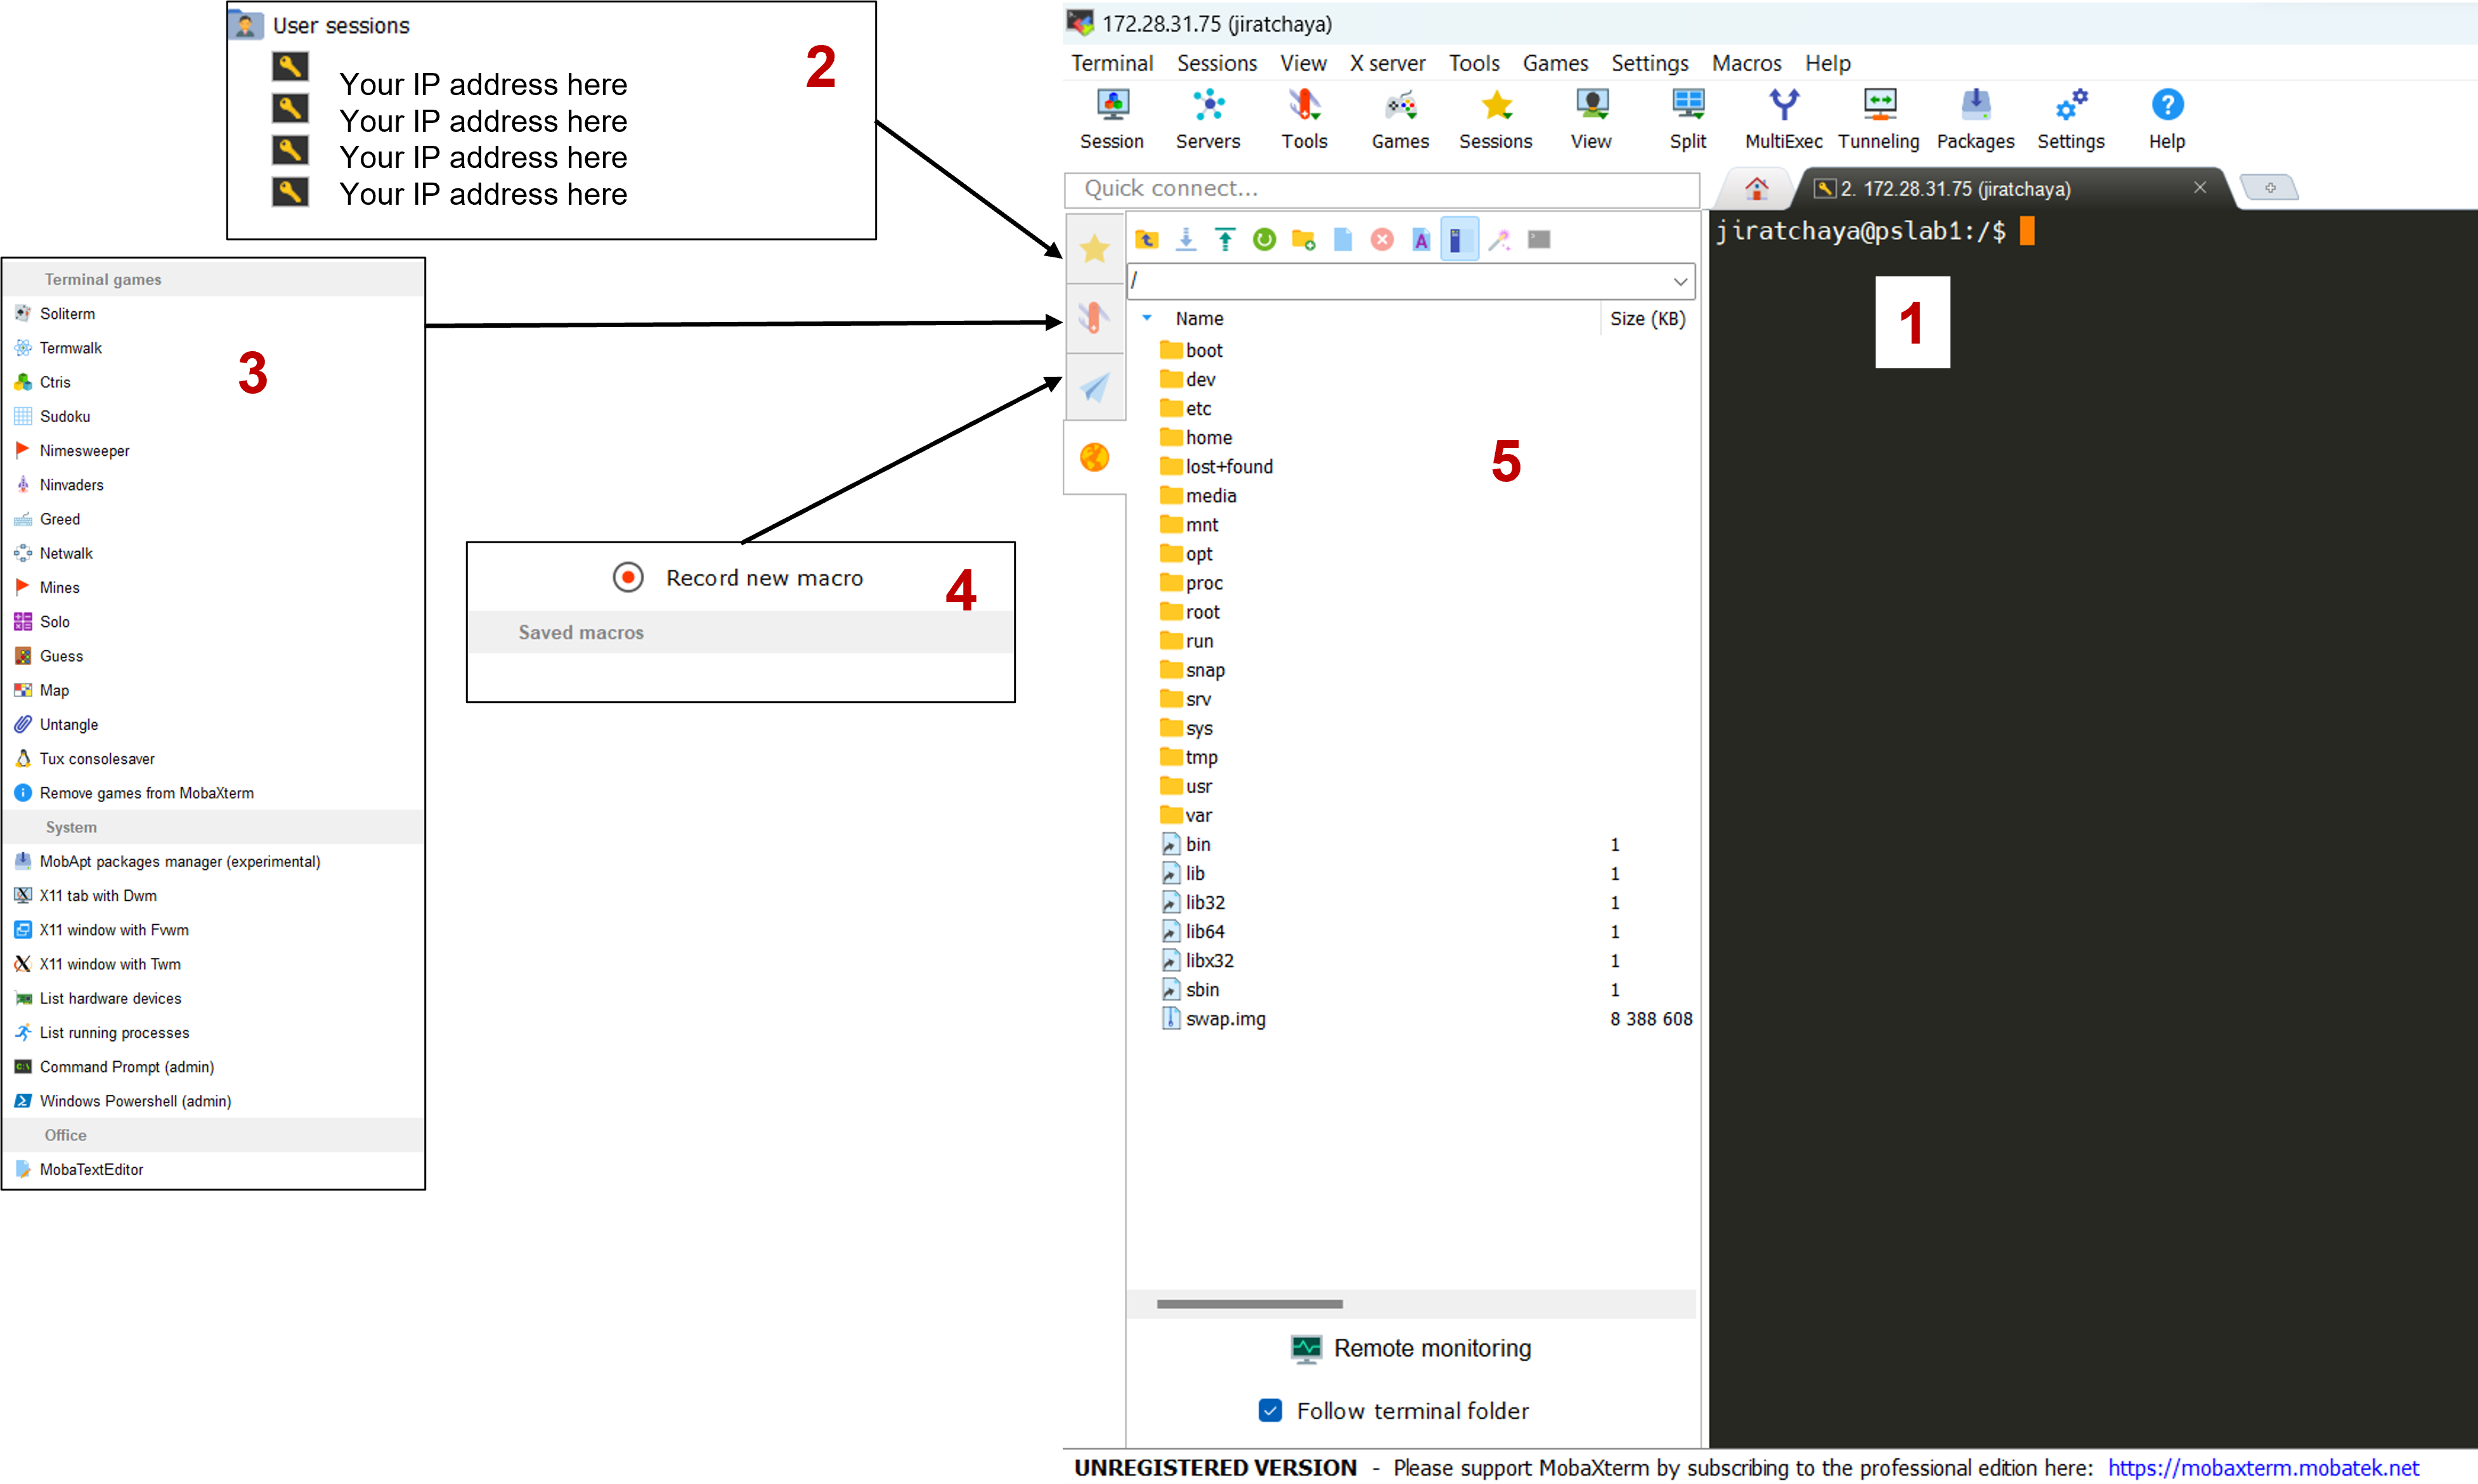
\includegraphics{./assets/01_moba_ui.png}

}

\caption{MobaXterm user interface. In the context of remote access
through SSH and FTP, mobaXterm provides easy-to-access route as (1) a
secure shell (SSH) terminal of the remote server, (2) a list of remote
server you've accessed, (3) Utilities facilitating remote server access
including entertainment, like Swiss army knife!, (4) If you want to
reduce redundant typing, just set macro to it, and (5) a files available
in the current working directory in the remote server, you can also
transfer files from remote server to your local computer using this
route!}

\end{figure}

There are many advantages of having an All-In-One network application
for your remote tasks, e.g.~when you use SSH to connect to a remote
server, a graphical SFTP browser will automatically pop up in order to
directly edit your remote files.

Visit MobaXterm official website to see a demo:
https://mobaxterm.mobatek.net/demo.html

\hypertarget{terminal-for-macos}{%
\section{Terminal (for macOS)}\label{terminal-for-macos}}

Terminal provides a command-line interface to macOS. Each window in
Terminal represents an instance of a shell process. The window contains
a prompt that indicates you can enter a command. The prompt you see
depends on your Terminal and shell settings, but it often includes the
name of the host you're logged in to, your current working folder, your
user name, and a prompt symbol. For example, if a user named michael is
using the default zsh shell, the prompt appears as:

\begin{verbatim}
michael@MacBook-Pro ~ %
\end{verbatim}

This indicates that the user named michael is logged in to a computer
named MacBook-Pro, and the current folder is his home folder, indicated
by the tilde (\textasciitilde).

MacOS features a built-in SSH client called Terminal which allows you to
quickly and easily connect to a server. Starting from open the
``terminal'' app, and enter the standard SSH command:

\begin{verbatim}
ssh user@IPAddress
\end{verbatim}

This will connect to the server via SSH with the username `user` and the
default SSH port 22. The connection will look similar to the following:

\hypertarget{connecting-to-remote-server}{%
\section{Connecting to Remote
Server}\label{connecting-to-remote-server}}

Bioinformatics data processing tasks require more computing power than
our laptops, so we need large servers or clusters. It's likely you'll
work mostly over a network connection with remote machines on some
projects. It can be frustrating for beginners to work with a remote
machine. So, This part will introduce you to some commonly used bash
commands. To make it easier for beginners to manage their remote
machines, there are a range of different tools and technologies
available, such as SSH, FTP, and terminal commands, which can be used to
access and manage the environment of the machine. Additionally, there
are a variety of bash commands which can be used to streamline the
process of managing the machine.

What you need to know for connecting to a remove server:

\begin{enumerate}
\def\labelenumi{\arabic{enumi}.}
\item
  Your username and password in the remote server
\item
  IP address of the remote server, and which port to connect to server
\item
  You should know whether the remote server accessible via local network
  or a public IP address
\end{enumerate}

By default, SSH uses port 22 but it can be changed to a non-standard
port. To securely connect the client to the remote server, SSH uses
symmetric encryption, asymmetric encryption, and hashing. If you're
connecting for the first time, you'll be asked to verify the server's
public key. Whenever you connect to the same server in the future, the
client will reference this verified public key. During an SSH
connection, the client and server negotiate a session key used to
encrypt and decrypt data.

\begin{figure}

{\centering 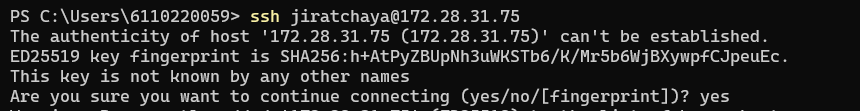
\includegraphics{./assets/02_ssh_authkeys.png}

}

\caption{In order to establish a connection, SSH needs to verify SHA
keys once connected for the first time. Once authentication is complete,
the SSH connection is secure and can be trusted for future access.}

\end{figure}

Upon connecting to the remote server, you'll see a welcome message like
this

\begin{figure}

{\centering 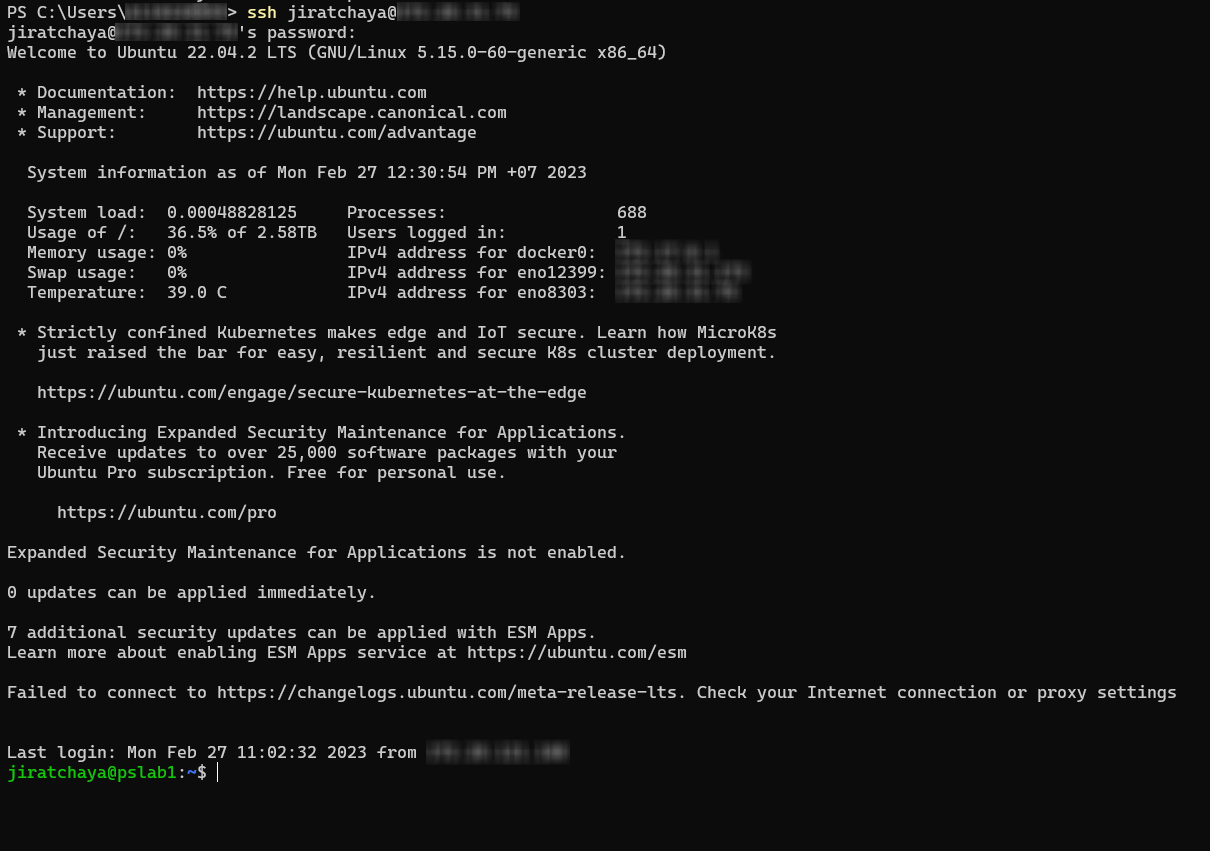
\includegraphics{./assets/03_ssh-welcome-message.png}

}

\caption{An example welcome message of server using Ubuntu, including
general software and hardware status, information of the latest
connection, as well as a prompt for user command.}

\end{figure}

\bookmarksetup{startatroot}

\hypertarget{bash-command-language-for-biologists}{%
\chapter{Bash Command Language for
Biologists}\label{bash-command-language-for-biologists}}

Shell scripts (or shell or UNIX) are widely used in bioinformatics
because they're the interface for large bioinformatics programs. In this
workshop, you'll learn how to use the necessary Bash command concepts.
This will allow you to focus on the content of the commands in the
following chapters rather than on understanding shell syntax. However,
before we start learning bash, it's good to understand Linux file
systems a little bit.

\hypertarget{linux-file-systems}{%
\section{Linux File Systems}\label{linux-file-systems}}

In Unix-like operating systems, the Linux file system defines the
directory structure and contents. Even if they're located on different
physical or virtual hard disks, all files and directories are located
under the root directory.

\begin{figure}

{\centering \includegraphics{https://media.geeksforgeeks.org/wp-content/uploads/linuxDir.jpg}

}

\caption{Schematic hierarchy of Linux file systems. The figure is
adopted from
\url{https://www.geeksforgeeks.org/linux-file-hierarchy-structure}.}

\end{figure}

\begin{description}
\item[Root (\texttt{/})]
It is the root directory of the entire file system hierarchy and the
primary hierarchy root. The root directory is where everything begins.
This directory can be written only by root.
\item[/bin]
Essential commands that must be available with all users, for example,
\texttt{cat}, \texttt{ls}, \texttt{cp}, \texttt{cd}, \texttt{top},
\texttt{mkdir} and many more.
\item[/dev]
Essential device files such as \texttt{/dev/null}, \texttt{/dev/shm}.
This includes terminal devices, USB or other devices connected to the
system.
\item[/etc]
System-wide configuration files for the host, contain files that all
programs need. Also included are startup and shutdown shell scripts for
starting and stopping individual programs, such as \texttt{/etc/fstab}
for permanently mounting external disks, \texttt{/etc/netplan} for
configuring the network and IP address, and more.
\item[/home]
Users' home directories, where they keep their saved files and settings.
These directories are used to store all of a user's files and settings
in one place so that they can easily access their data and keep it
organized. For example \texttt{/home/ponsit}, \texttt{/home/jiratchaya},
\texttt{/home/prasert}.
\item[/lib]
Contain essential libraries for the binaries in \texttt{/bin/} and
\texttt{/sbin/}.
\item[/media]
Mount points for removable media such as CD-ROMs (deprecated).
\item[/mnt]
Temporary mount directory where sysadmins can mount file systems, such
as \texttt{/mnt/external\_disk\_1}, \texttt{/mnt/removable\_drive\_1},
etc.
\item[/opt]
Optional application software packages, including add-on applications
from individual vendors.
\item[/sbin]
Essential system binaries, e.g., \texttt{fsck}, \texttt{init}, route.
\item[/tmp]
Temporary files that aren't preserved between reboots and may be
severely restricted.
\item[/usr]
A secondary hierarchy for read-only user data. Most utilities and
applications are located here.
\end{description}

\hypertarget{basic-bash-commands}{%
\section{Basic Bash Commands}\label{basic-bash-commands}}

Bash is a Unix shell that allows you to enter commands that are then
interpreted and executed by the computer. Commands can be used to
perform tasks such as creating a directory, running a program, or
deleting a file. Bash is a type of interpreter that takes user input and
converts it into a language that the computer can understand and
execute. Commands usually consist of keywords, arguments, and flags that
allow the user to control how the command is interpreted and executed by
the computer.

\hypertarget{creating-directories}{%
\subsection*{Creating directories}\label{creating-directories}}
\addcontentsline{toc}{subsection}{Creating directories}

Keeping all your files in a single directory makes things much easier
for you and your collaborators, and makes it easier to reproduce.
Suppose you're working on a transcriptome analysis of \emph{Cyanophora
paradoxa}. Your first step would be to choose a short, appropriate
project name and create some basic directories.

\begin{quote}
🗒️\textbf{Note:} In Linux file system, \textbf{directory} is exactly the
same with \textbf{folder}.
\end{quote}

To keep it short and clear, `Cpa' is used as an alias article name for
\emph{C. paradoxa}, and as the name of the directory, followed by words
describing your work, for example.

\begin{quote}
⚠️ \textbf{warning:} Avoid using spaces ( ) or special characters such
as slashes ( / ), backslashes ( \textbackslash{} ), accented characters
( ' ), tilde ( \textasciitilde{} ), and many others. It is
\textbf{recommended to use underscore ( \_ )} or hyphen ( - ) instead of
these special characters.
\end{quote}

\begin{itemize}
\tightlist
\item
  Create a directory name `Cpa\_RNASeq' from current working directory
\end{itemize}

\begin{Shaded}
\begin{Highlighting}[]
\FunctionTok{mkdir}\NormalTok{ Cpa\_RNASeq}
\end{Highlighting}
\end{Shaded}

This will create a directory named `Cpa\_RNASeq' in your current working
directory. Let us create some subdirectories!

\begin{itemize}
\tightlist
\item
  Create subdirectory `01\_Rawdata' under the `Cpa\_RNASeq' directory
\end{itemize}

\begin{Shaded}
\begin{Highlighting}[]
\FunctionTok{mkdir}\NormalTok{ Cpa\_RNASeq/01\_Rawdata}
\end{Highlighting}
\end{Shaded}

This will create a subdirectory name `01\_Rawdata' in the directory
`Cpa\_RNASeq'

\begin{itemize}
\tightlist
\item
  Create multiple directory at once
\end{itemize}

For example, if you want to create 2 directories named `02\_QC' and
`03\_assembly' under the `Cpa\_RNASeq' directory, then simply type

\begin{Shaded}
\begin{Highlighting}[]
\FunctionTok{mkdir}\NormalTok{ Cpa\_RNASeq/}\DataTypeTok{\{02\_QC}\OperatorTok{,}\DataTypeTok{03\_assembly\}}
\end{Highlighting}
\end{Shaded}

\begin{tcolorbox}[enhanced jigsaw, breakable, bottomrule=.15mm, left=2mm, coltitle=black, opacityback=0, colframe=quarto-callout-note-color-frame, toprule=.15mm, opacitybacktitle=0.6, colbacktitle=quarto-callout-note-color!10!white, bottomtitle=1mm, colback=white, toptitle=1mm, titlerule=0mm, rightrule=.15mm, arc=.35mm, title=\textcolor{quarto-callout-note-color}{\faInfo}\hspace{0.5em}{Activity}, leftrule=.75mm]

A well-organized project directory can make life easier. Your project
directory should be organized in a consistent and understandable way. A
clear project organization makes it easier for both you and your
collaborators to find out exactly where and what everything is located,
which improves the reproducibility of research. It's also much easier to
automate tasks when files are organized and clearly named.

In this workshop, we'll learn transcriptome data analysis in many steps
from downloading reads to transcriptome annotation. Therefore, we'll
divide each analysis step into subdirectories as follows. Let's assume
that we have already created the directory \texttt{Cpa\_RNASeq}.

\begin{verbatim}
.
└── Cpa_RNASeq
    ├── 01_Rawdata
    ├── 02_QC
    ├── 03_assembly
    ├── 04_DE_analysis
    └── 05_annotation
\end{verbatim}

Could you generate bash command(s) to create these directories ?

\end{tcolorbox}

\begin{tcolorbox}[enhanced jigsaw, breakable, bottomrule=.15mm, left=2mm, coltitle=black, opacityback=0, colframe=quarto-callout-caution-color-frame, toprule=.15mm, opacitybacktitle=0.6, colbacktitle=quarto-callout-caution-color!10!white, bottomtitle=1mm, colback=white, toptitle=1mm, titlerule=0mm, rightrule=.15mm, arc=.35mm, title=\textcolor{quarto-callout-caution-color}{\faFire}\hspace{0.5em}{Answer}, leftrule=.75mm]

\begin{Shaded}
\begin{Highlighting}[]
\FunctionTok{mkdir}\NormalTok{ Cpa\_RNASeq/}\DataTypeTok{\{01\_Rawdata}\OperatorTok{,}\DataTypeTok{02\_QC}\OperatorTok{,}\DataTypeTok{03\_assembly}\OperatorTok{,}\DataTypeTok{04\_DE\_analysis}\OperatorTok{,}\DataTypeTok{05\_annotation\}}
\end{Highlighting}
\end{Shaded}

or

\begin{Shaded}
\begin{Highlighting}[]
\FunctionTok{mkdir}\NormalTok{ Cpa\_RNASeq/01\_Rawdata Cpa\_RNASeq/02\_QC Cpa\_RNASeq/03\_assembly Cpa\_RNASeq/04\_DE\_analysis Cpa\_RNASeq/05\_annotation}
\end{Highlighting}
\end{Shaded}

or

\begin{Shaded}
\begin{Highlighting}[]
\BuiltInTok{cd}\NormalTok{ Cpa\_RNASeq}
\FunctionTok{mkdir}\NormalTok{ 01\_Rawdata 02\_QC 03\_assembly 04\_DE\_analysis 05\_annotation}
\end{Highlighting}
\end{Shaded}

\end{tcolorbox}

\hypertarget{navigating-your-file-system}{%
\subsection*{Navigating your file
system}\label{navigating-your-file-system}}
\addcontentsline{toc}{subsection}{Navigating your file system}

The file system manages the files and directories of the operating
system. It organizes our data into files, which store information, and
directories. When you see the prompt below on your terminal's screen, it
means that your terminal has processed the command you entered and is
ready for the next command.

\begin{Shaded}
\begin{Highlighting}[]
\ExtensionTok{jiratchaya@DESKTOP{-}P2DD13C:\textasciitilde{}$}
\end{Highlighting}
\end{Shaded}

\texttt{jiratchaya} is username using this terminal. The address @
symbol followed by \texttt{DESKTOP-P2DD13C} in a computer or server
name. And, the dollar sign \texttt{\$} is a prompt, which shows us that
the shell is waiting for input. Your shell may use a different character
as a prompt and may add information before the prompt.

If you want to find out where we are now, type

\begin{Shaded}
\begin{Highlighting}[]
\BuiltInTok{pwd}
\end{Highlighting}
\end{Shaded}

pwd stands for print working directory. Without explicit specification,
the computer assumes that we want to execute commands in our current
working directory. This can be a user's home directory
(\texttt{\textasciitilde{}}).

If you want to change the directory, e.g.~to the `Cpa\_RNASeq' directory
we just created, just type the following

\begin{Shaded}
\begin{Highlighting}[]
\BuiltInTok{cd}\NormalTok{ Cpa\_RNASeq}
\end{Highlighting}
\end{Shaded}

\texttt{cd} stands for ``change directory''. You can change our working
directory by typing \texttt{cd} followed by a directory name. In this
case you change from the current directory to the directory named
`Cpa\_RNASeq'.

\hypertarget{listing-directories}{%
\subsection*{Listing directories}\label{listing-directories}}
\addcontentsline{toc}{subsection}{Listing directories}

We can see what files and subdirectories are in this directory by
running ls, which stands for ``listing'':

\begin{Shaded}
\begin{Highlighting}[]
\FunctionTok{ls}
\end{Highlighting}
\end{Shaded}

Expected result:

\begin{verbatim}
jiratchaya@DESKTOP-P2DD13C:~/Cpa_RNASeq$ ls
01_Rawdata  02_QC  03_assembly
\end{verbatim}

Let us look at the other way. This way is to list all the files and
directories, including the users who own them, the permissions, and the
file size in bytes.

\begin{Shaded}
\begin{Highlighting}[]
\FunctionTok{ls} \AttributeTok{{-}l}
\end{Highlighting}
\end{Shaded}

Expected result:

\begin{verbatim}
jiratchaya@DESKTOP-P2DD13C:~/Cpa_RNASeq$ ls -l
total 12
drwxr-xr-x 2 jiratchaya jiratchaya 4096 Mar  1 21:02 01_Rawdata
drwxr-xr-x 2 jiratchaya jiratchaya 4096 Mar  1 21:02 02_QC
drwxr-xr-x 2 jiratchaya jiratchaya 4096 Mar  1 21:02 03_assembly
\end{verbatim}

List files and folders, permissions and size in a human readable format.

\begin{Shaded}
\begin{Highlighting}[]
\FunctionTok{ls} \AttributeTok{{-}lh}
\end{Highlighting}
\end{Shaded}

Expected result:

\begin{verbatim}
jiratchaya@DESKTOP-P2DD13C:~/Cpa_RNASeq$ ls -l
total 12
drwxr-xr-x 2 jiratchaya jiratchaya 4096 Mar  1 21:02 01_Rawdata
drwxr-xr-x 2 jiratchaya jiratchaya 4096 Mar  1 21:02 02_QC
drwxr-xr-x 2 jiratchaya jiratchaya 4096 Mar  1 21:02 03_assembly
\end{verbatim}

See all hidden files and directories

\begin{Shaded}
\begin{Highlighting}[]
\FunctionTok{ls} \AttributeTok{{-}la}
\end{Highlighting}
\end{Shaded}

Expected result:

\begin{verbatim}
jiratchaya@DESKTOP-P2DD13C:~/Cpa_RNASeq$ ls -la
total 20
drwxr-xr-x 5 jiratchaya jiratchaya 4096 Mar  1 21:02 .
drwxr-x--- 3 jiratchaya jiratchaya 4096 Mar  1 21:02 ..
drwxr-xr-x 2 jiratchaya jiratchaya 4096 Mar  1 21:02 01_Rawdata
drwxr-xr-x 2 jiratchaya jiratchaya 4096 Mar  1 21:02 02_QC
drwxr-xr-x 2 jiratchaya jiratchaya 4096 Mar  1 21:02 03_assembly
\end{verbatim}

\hypertarget{files-and-directories-handling}{%
\subsection*{Files and directories
handling}\label{files-and-directories-handling}}
\addcontentsline{toc}{subsection}{Files and directories handling}

\hypertarget{creating-and-editing-files}{%
\subsubsection*{Creating and editing
files}\label{creating-and-editing-files}}
\addcontentsline{toc}{subsubsection}{Creating and editing files}

When you work on the command line, you often need to create or edit text
files. In this workshop, we recommend using \texttt{nano} as a text
editor. Other Unix text editors you may have heard of include vi, vim,
emacs, vscode, and many more.

We'll create the file \texttt{test.fasta}. To open an existing file or
create a new file, type nano followed by the filename:

\begin{Shaded}
\begin{Highlighting}[]
\FunctionTok{nano}\NormalTok{ test.fasta}
\end{Highlighting}
\end{Shaded}

This will bring up the text editing screen on your terminal. Here you
can type anything you want, but in this case we'll create a sequence
like this.

\begin{verbatim}
>seq_01
TCGCTAGTC

>seq_02
TAGCGAGTT
\end{verbatim}

\begin{quote}
🗒️\textbf{Note:}Always leave an enter in the last line. This is
advantageous if this file is further used by many programmes.
\end{quote}

\begin{figure}

{\centering 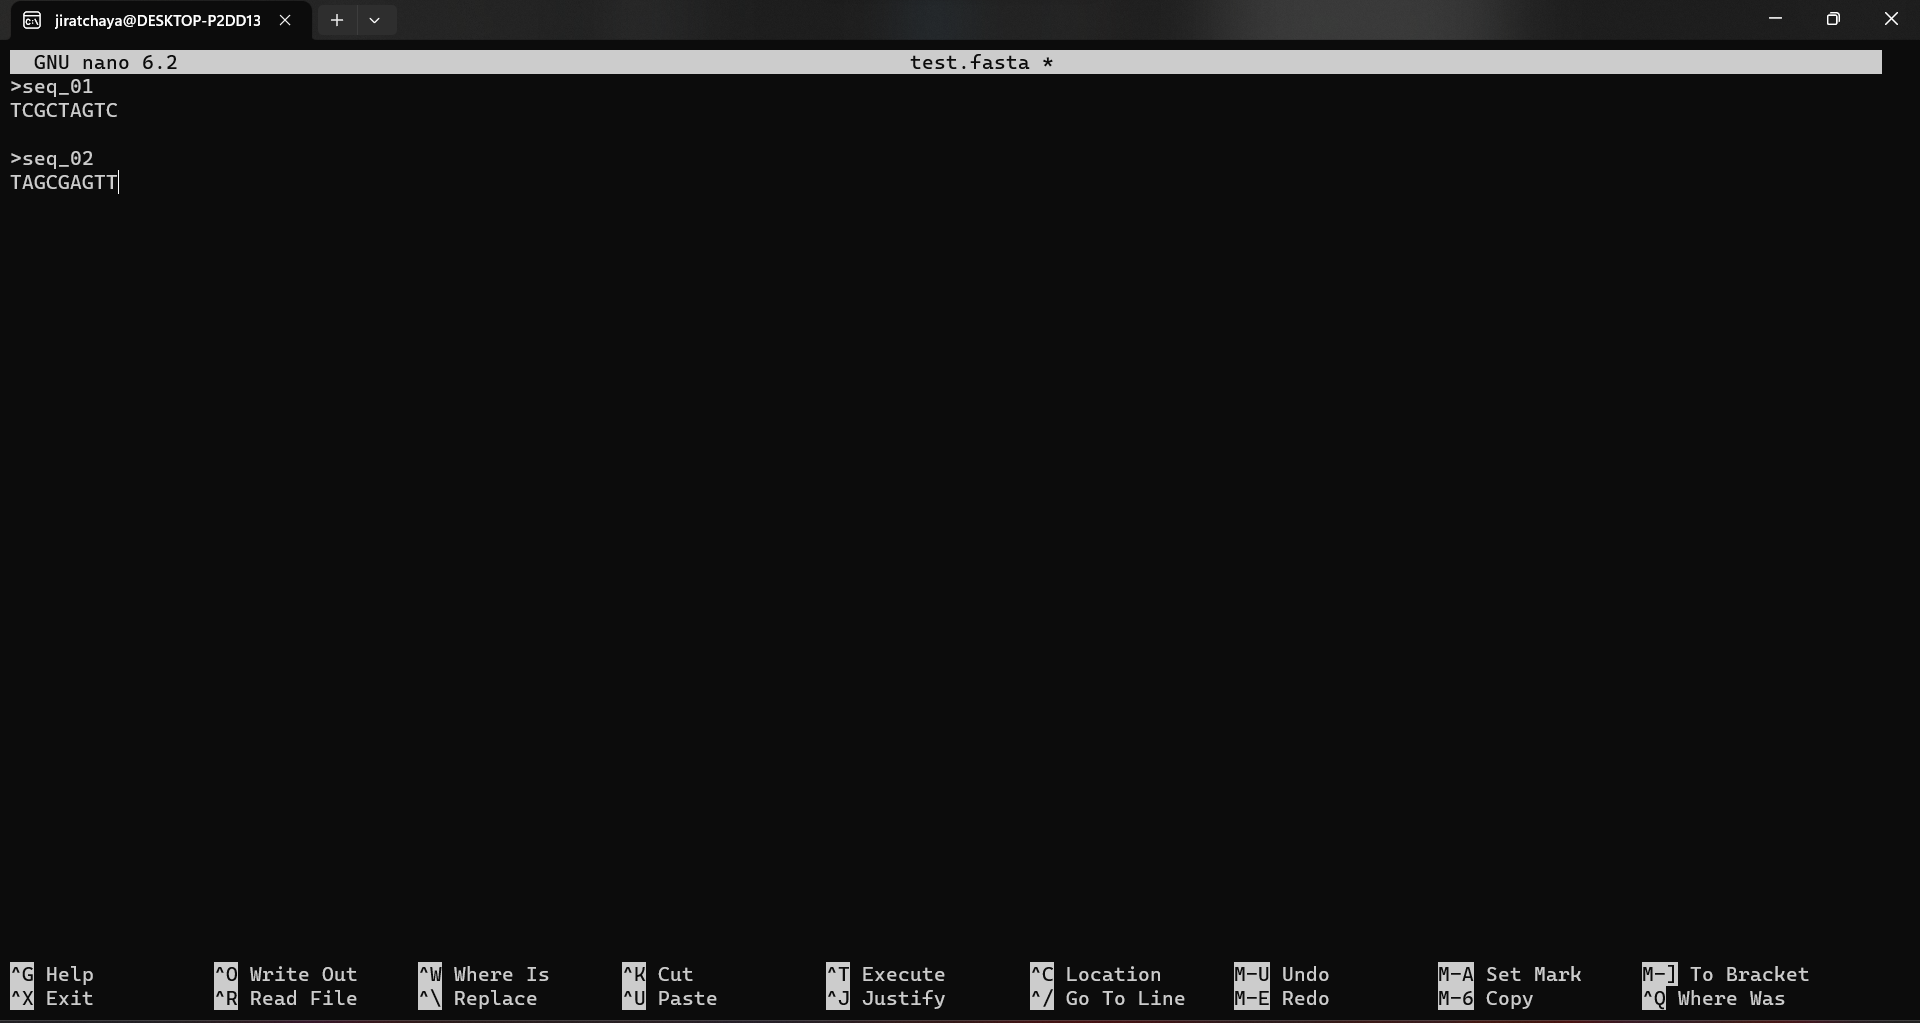
\includegraphics{./assets/04_nano_screen.png}

}

\caption{The text editing screen is displayed once you have typed nano
into some files. At the bottom of the window is a list of the most
important keyboard shortcuts for the nano editor. All commands are
preceded by either a \texttt{\^{}} or an \texttt{M} character. The caret
symbol (\texttt{\^{}}) stands for the \texttt{Ctrl} key. For example,
the commands \texttt{\^{}J} mean that you press the \texttt{Ctrl} and
\texttt{J} keys simultaneously. The letter \texttt{M} stands for the
\texttt{Alt} key.}

\end{figure}

To edit a file, you can use the navigation keys such as arrow keys, End,
Home, PgUp or PgDn to control the cursor.

To save the changes you made to the file, press \texttt{Ctrl+o}. If the
file doesn't exist yet, it'll be created after saving.

To exit nano, press \texttt{Ctrl+x}. If there are unsaved changes,
you'll be asked if you want to save the changes. Nano will ask you `Save
modified buffer?', then type \texttt{y} to confirm the edit.

\hypertarget{copying-files-and-directories}{%
\subsubsection*{Copying files and
directories}\label{copying-files-and-directories}}
\addcontentsline{toc}{subsubsection}{Copying files and directories}

To copy files and directories the command \texttt{cp} can be used.
\texttt{cp} stands for copy and is used to copy files and directories in
Linux. An example: You copy the file \texttt{test.fasta} to
\texttt{01\_Rawdata} with the following syntax

\begin{verbatim}
cp [source file] [target_directory]/
\end{verbatim}

For example

\begin{Shaded}
\begin{Highlighting}[]
\FunctionTok{cp}\NormalTok{ test.fasta 01\_Rawdata/}
\end{Highlighting}
\end{Shaded}

Copy file to another file, using the syntax

\begin{verbatim}
cp [source_file] [new_file_name]
\end{verbatim}

For example

\begin{Shaded}
\begin{Highlighting}[]
\FunctionTok{cp}\NormalTok{ test.fasta test\_2.fasta}
\end{Highlighting}
\end{Shaded}

You can copy a file to a new file in the directory by using the
following syntax

\begin{verbatim}
cp [source_file] [target_directory]/[new_file_name]
\end{verbatim}

For example

\begin{Shaded}
\begin{Highlighting}[]
\FunctionTok{cp}\NormalTok{ test.fasta 01\_Rawdata/another\_test.fasta}
\end{Highlighting}
\end{Shaded}

To copying directory, use additional flag as follow

\begin{verbatim}
cp -r [source_directory] [new_directory_name]
\end{verbatim}

The flag \texttt{-r} stands for recursive, i.e.~all files and
subdirectories in this directory are copied repeatedly. For example,
\texttt{01\_Rawdata} already contains \texttt{test.fasta}, which we
copied before, and we want to duplicate this directory.

\begin{Shaded}
\begin{Highlighting}[]
\FunctionTok{cp} \AttributeTok{{-}r}\NormalTok{ 01\_Rawdata/ 01\_Rawdata\_new}
\end{Highlighting}
\end{Shaded}

\hypertarget{moving-files-and-directories}{%
\subsubsection*{Moving files and
directories}\label{moving-files-and-directories}}
\addcontentsline{toc}{subsubsection}{Moving files and directories}

To copy files and directories, the command \texttt{mv} can be used.
\texttt{mv} stands for move and is used to move files and directories in
Linux. For example, move the file \texttt{test\_2.fasta} to the
directory \texttt{01\_Rawdata\_new} with the following syntax

\begin{verbatim}
mv [file_to_move] [target_directory]
\end{verbatim}

\begin{Shaded}
\begin{Highlighting}[]
\FunctionTok{mv}\NormalTok{ test\_2.fasta 01\_Rawdata\_new/}
\end{Highlighting}
\end{Shaded}

Specifically, to move files and directories, no flags are required as
with \texttt{cp}. So if we want to move \texttt{01\_Rawdata\_new} to a
subdirectory of \texttt{01\_Rawdata}, this can be done as follows

\begin{verbatim}
mv [source_file_or_dir] [target_file_or_dir]
\end{verbatim}

\begin{Shaded}
\begin{Highlighting}[]
\FunctionTok{mv}\NormalTok{ 01\_Rawdata\_new/ 01\_Rawdata}
\end{Highlighting}
\end{Shaded}

Moving file within the directory up to the current directory

\begin{verbatim}
mv [source_dir]/[source_file] .
\end{verbatim}

The dot ( . ) stands for the current directory, which means you want to
move something to the current directory. For example, we want to move
the file \texttt{another\_test.fasta}, which is in the directory
\texttt{01\_Rawdata}, to the current directory by typing

\begin{Shaded}
\begin{Highlighting}[]
\FunctionTok{mv}\NormalTok{ 01\_Rawdata/another\_test.fasta .}
\end{Highlighting}
\end{Shaded}

\hypertarget{deleting-files-and-directories}{%
\subsubsection*{Deleting files and
directories}\label{deleting-files-and-directories}}
\addcontentsline{toc}{subsubsection}{Deleting files and directories}

Removing files and directories can be done with the command \texttt{rm}.
\texttt{rm} stands for remove and is used to delete files and
directories in Linux. It's simple and straightforward with the following
syntax.

\begin{verbatim}
rm [file_to_delete]
\end{verbatim}

For example, you are deleting file \texttt{another\_test.fasta}

\begin{Shaded}
\begin{Highlighting}[]
\FunctionTok{rm}\NormalTok{ another\_test.fasta}
\end{Highlighting}
\end{Shaded}

To delete directories, use additional flags

\begin{verbatim}
rm -rf [directory_to_delete]
\end{verbatim}

The flag \texttt{-r} means that it does something recursive, which means
that it deletes all files and subdirectories of the directory you want
to delete. The flag \texttt{f} can help us delete some protected files
and directories that you should think twice before deleting.

For example you want to delete \texttt{03\_adapter\_trimming} directory

\begin{Shaded}
\begin{Highlighting}[]
\FunctionTok{rm} \AttributeTok{{-}rf}\NormalTok{ 03\_adapter\_trimming}
\end{Highlighting}
\end{Shaded}

Or delete subdirectory \texttt{01\_Rawdata\_new} by

\begin{Shaded}
\begin{Highlighting}[]
\FunctionTok{rm} \AttributeTok{{-}rf}\NormalTok{ 01\_Rawdata/01\_Rawdata\_new}
\end{Highlighting}
\end{Shaded}

Don't worry\textasciitilde{} the \texttt{01\_Rawdata} is still with us

\begin{verbatim}
jiratchaya@DESKTOP-P2DD13C:~/Cpa_RNASeq$ ls -l
total 20
drwxr-xr-x 2 jiratchaya jiratchaya 4096 Mar  1 22:33 01_Rawdata
drwxr-xr-x 2 jiratchaya jiratchaya 4096 Mar  1 21:59 02_QC
-rw-r--r-- 1 jiratchaya jiratchaya   38 Mar  1 22:00 another_test.fasta
-rw-r--r-- 1 jiratchaya jiratchaya   38 Mar  1 21:59 test.fasta
-rw-r--r-- 1 jiratchaya jiratchaya   38 Mar  1 22:00 test_2.fasta
\end{verbatim}

\begin{quote}
🚨 \textbf{Danger zone:} Be sure to check the path of the location where
you want to delete something with the command \texttt{rm\ -rf},
otherwise you'll unintentionally delete necessary files or directories.

\begin{figure}

{\centering 

\href{https://www.reddit.com/r/linuxmemes/comments/gk8k2x/why_i_prefer_using_rm_i_or_deleting_the_entire/}{\includegraphics[width=0.7\textwidth,height=\textheight]{https://i.redd.it/346ib6l1exy41.png}}

}

\end{figure}
\end{quote}

\hypertarget{downloading-file-from-url}{%
\subsection*{Downloading file from
URL}\label{downloading-file-from-url}}
\addcontentsline{toc}{subsection}{Downloading file from URL}

There are numerous ways to download a file from a URL via the command
line on Linux, and two of the best tools for this task are \texttt{wget}
and \texttt{curl}. Both tools have their advantages and disadvantages,
depending on the download task at hand. However, in this workshop we'll
mainly focus on downloading with \texttt{curl}.

For example, we want to download the latest (draft) genome assembly
report of \emph{Cyanophora paradoxa} from the NCBI genome database via
\texttt{curl} as follows.

\begin{Shaded}
\begin{Highlighting}[]
\ExtensionTok{curl} \AttributeTok{{-}O}\NormalTok{ https://ftp.ncbi.nlm.nih.gov/genomes/all/GCA/004/431/415/GCA\_004431415.1\_ASM443141v1/GCA\_004431415.1\_ASM443141v1\_assembly\_report.txt}
\end{Highlighting}
\end{Shaded}

Expected output

\begin{verbatim}
jiratchaya@DESKTOP-P2DD13C:~/Cpa_RNASeq$ curl -O https://ftp.ncbi.nlm.nih.gov/genomes/all/GCA/004/431/415/GCA_004431415.1_ASM443141v1/GCA_004431415.1_ASM443141v1_assembly_report.txt
  % Total    % Received % Xferd  Average Speed   Time    Time     Time  Current
                                 Dload  Upload   Total   Spent    Left  Speed
100 61357  100 61357    0     0  21604      0  0:00:02  0:00:02 --:--:-- 21604
jiratchaya@DESKTOP-P2DD13C:~/Cpa_RNASeq$ ls -l
total 80
drwxr-xr-x 2 jiratchaya jiratchaya  4096 Mar  1 22:33 01_Rawdata
drwxr-xr-x 2 jiratchaya jiratchaya  4096 Mar  1 21:59 02_QC
-rw-r--r-- 1 jiratchaya jiratchaya 61357 Mar  1 22:56 GCA_004431415.1_ASM443141v1_assembly_report.txt
-rw-r--r-- 1 jiratchaya jiratchaya    38 Mar  1 22:00 another_test.fasta
-rw-r--r-- 1 jiratchaya jiratchaya    38 Mar  1 21:59 test.fasta
-rw-r--r-- 1 jiratchaya jiratchaya    38 Mar  1 22:00 test_2.fasta
\end{verbatim}

\textbf{Tips:} The alternative way to retrieve genome information from
NCBI, you can just go to
\href{https://www.ncbi.nlm.nih.gov/data-hub/genome/}{NCBI Genome Data
Hub} and specify species name to get information. NCBI provides several
routes to download files including \texttt{curl}!

\begin{figure}

{\centering 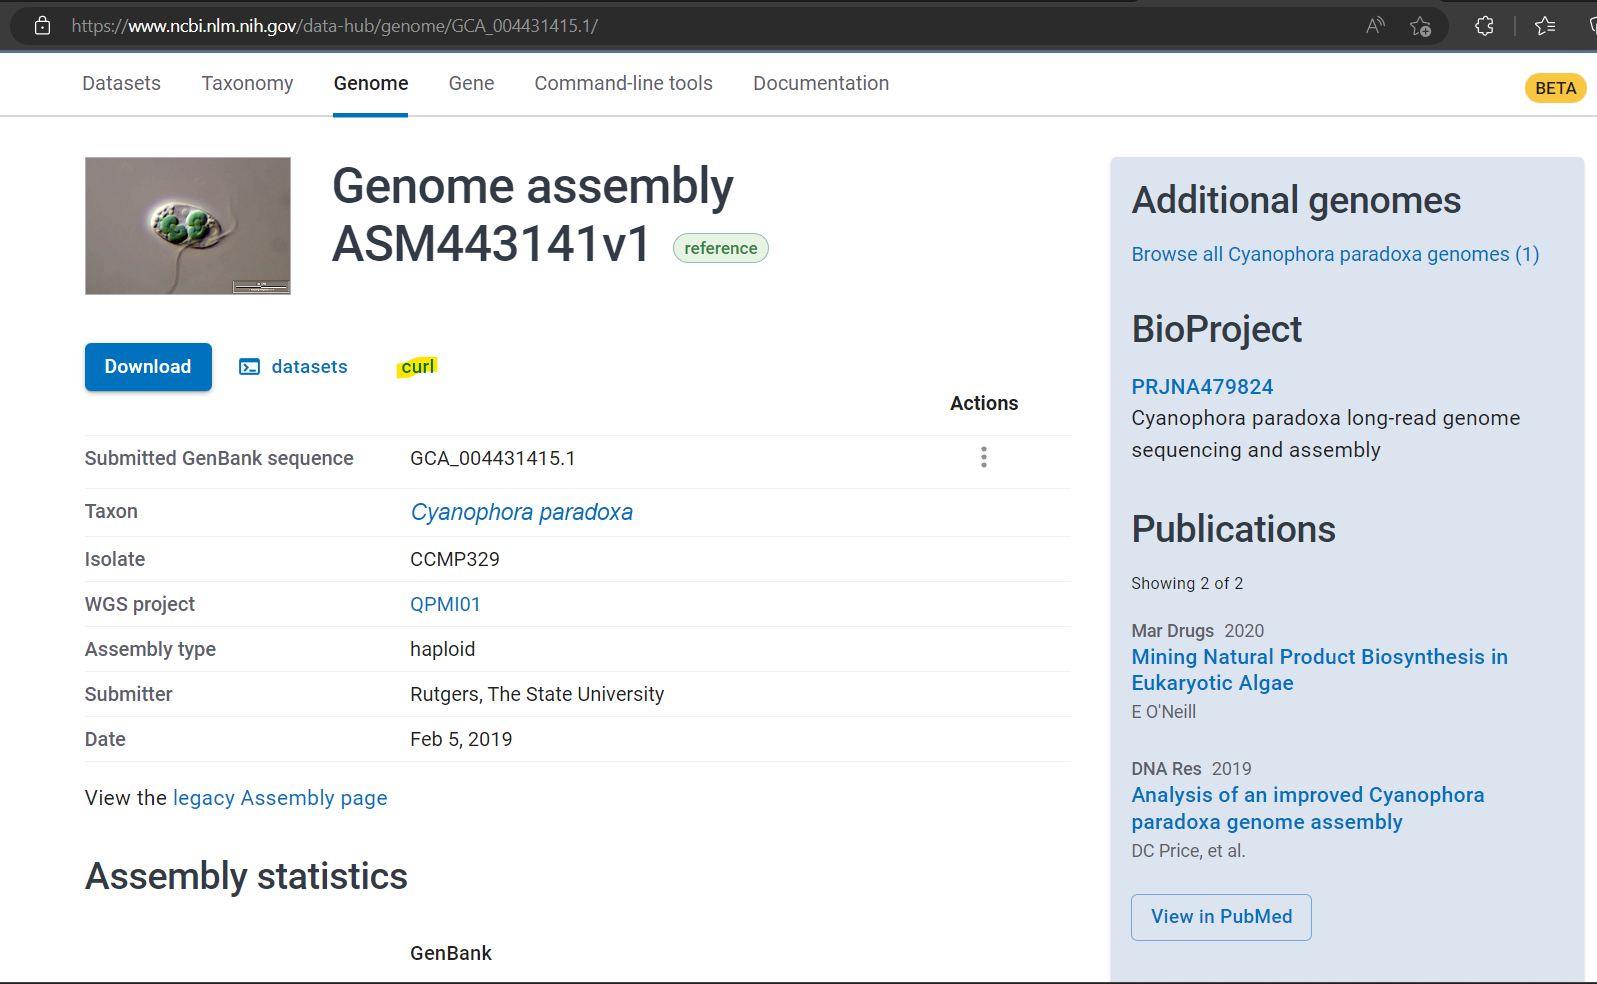
\includegraphics{./assets/05_genome_data_hub.png}

}

\caption{A genome assembly of \emph{C. paradoxa} in NCBI genome data hub
(Accessed: 1 March 2023)}

\end{figure}

\hypertarget{inspecting-file}{%
\subsection*{Inspecting file}\label{inspecting-file}}
\addcontentsline{toc}{subsection}{Inspecting file}

We'll inspect the assembly report file
\texttt{GCA\_004431415.1\_ASM443141v1\_assembly\_report.txt} that we
just downloaded from NCBI

\begin{itemize}
\tightlist
\item
  Count how many lines in that file
\end{itemize}

\begin{Shaded}
\begin{Highlighting}[]
\FunctionTok{wc} \AttributeTok{{-}l}\NormalTok{ GCA\_004431415.1\_ASM443141v1\_assembly\_report.txt}
\end{Highlighting}
\end{Shaded}

\begin{verbatim}
jiratchaya@DESKTOP-P2DD13C:~/Cpa_RNASeq$ wc -l GCA_004431415.1_ASM443141v1_assembly_report.txt
743 GCA_004431415.1_ASM443141v1_assembly_report.txt
\end{verbatim}

\begin{itemize}
\tightlist
\item
  Print some contents at a time.
\end{itemize}

Now you will see the number of lines that fit on your screen, and you
can scroll \texttt{up} and \texttt{down} with the arrow keys. Then press
\texttt{q} when you have checked your file.

\begin{Shaded}
\begin{Highlighting}[]
\FunctionTok{less}\NormalTok{ GCA\_004431415.1\_ASM443141v1\_assembly\_report.txt}
\end{Highlighting}
\end{Shaded}

\begin{figure}

{\centering 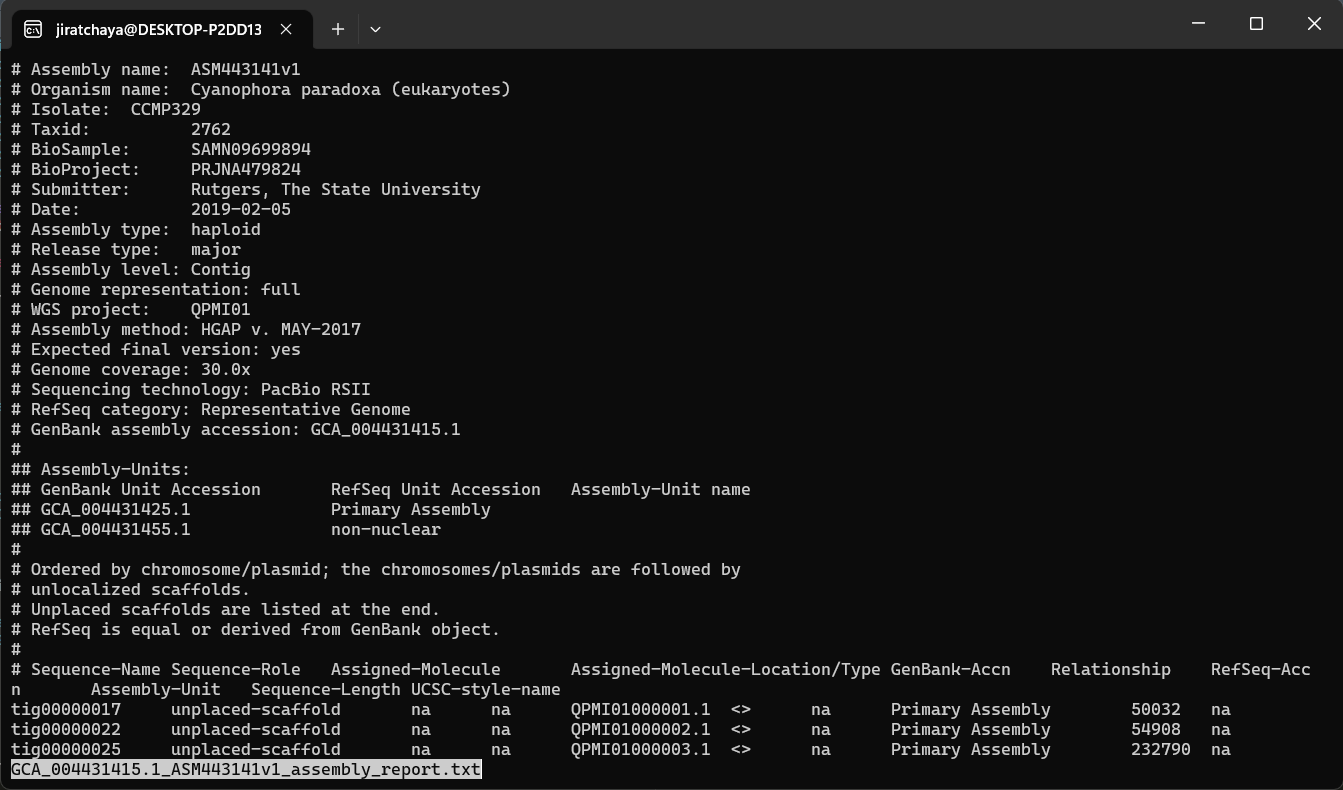
\includegraphics[width=1\textwidth,height=\textheight]{./assets/06_less_file.png}

}

\caption{Example of inspecting a file with the \texttt{less} command.
Users can scroll up and down with the arrow keys and exit by pressing
\texttt{q}.}

\end{figure}

\begin{itemize}
\tightlist
\item
  Print top 10 lines of file
\end{itemize}

\begin{Shaded}
\begin{Highlighting}[]
\FunctionTok{head}\NormalTok{ GCA\_004431415.1\_ASM443141v1\_assembly\_report.txt}
\end{Highlighting}
\end{Shaded}

\begin{figure}

{\centering 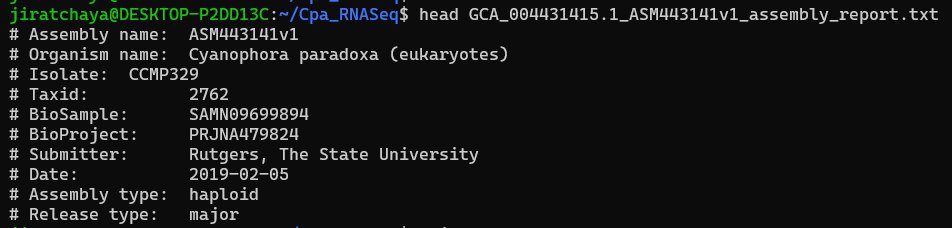
\includegraphics{./assets/07_head_file.png}

}

\caption{The first 10 lines of \emph{C. paradoxa} assembly report file}

\end{figure}

\begin{itemize}
\tightlist
\item
  Print bottom 10 lines of file
\end{itemize}

\begin{Shaded}
\begin{Highlighting}[]
\FunctionTok{tail}\NormalTok{ GCA\_004431415.1\_ASM443141v1\_assembly\_report.txt}
\end{Highlighting}
\end{Shaded}

\begin{figure}

{\centering 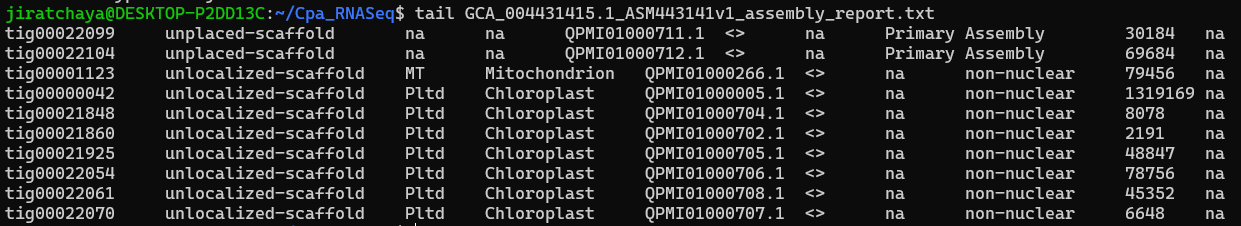
\includegraphics[width=1\textwidth,height=\textheight]{./assets/08_tail_file.png}

}

\caption{The last 10 lines of \emph{C. paradoxa} assembly report file.}

\end{figure}

\begin{itemize}
\tightlist
\item
  Print only lines with a specific pattern of word.
\end{itemize}

For example, we'll print only the lines contain the word ``Chloroplast''

\begin{Shaded}
\begin{Highlighting}[]
\FunctionTok{grep} \StringTok{"Chloroplast"}\NormalTok{ GCA\_004431415.1\_ASM443141v1\_assembly\_report.txt}
\end{Highlighting}
\end{Shaded}

\begin{figure}

{\centering 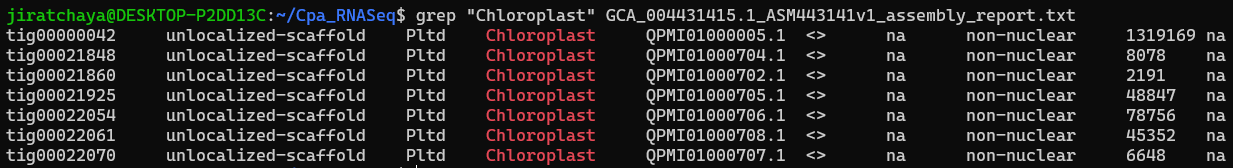
\includegraphics{./assets/09_grep_file.png}

}

\caption{Extracted lines with a specific word ``Chloroplast'' in
assembly report file.}

\end{figure}

\hypertarget{show-latest-commands-we-used}{%
\subsection*{Show latest commands we
used}\label{show-latest-commands-we-used}}
\addcontentsline{toc}{subsection}{Show latest commands we used}

You can simply press arrow keys \texttt{up} or \texttt{down} to see your
latest commands that you typed in the terminal.

Another way to see the latest command by typing below in the terminal

\begin{Shaded}
\begin{Highlighting}[]
\BuiltInTok{history}
\end{Highlighting}
\end{Shaded}

History is able to keep track of the command lines you use, associate
any data with each line, and use information from previous lines when
writing new lines.

\hypertarget{shortcut-tab-completion}{%
\subsection*{Shortcut: Tab Completion}\label{shortcut-tab-completion}}
\addcontentsline{toc}{subsection}{Shortcut: Tab Completion}

When typing file or directory names, it's easy to mistype. Instead, we
can use `tab' to complete what we want to type. The shell will try to
fill in the rest of a directory or file name if you press tab after
typing.

\begin{figure}

{\centering \includegraphics{https://i.stack.imgur.com/jKJz0.gif}

}

\caption{Using tab autocomplete in bash.}

\end{figure}

\hypertarget{have-no-idea-what-this-command-can-do}{%
\subsection{Have no idea what this command can
do}\label{have-no-idea-what-this-command-can-do}}

Basically, the built-in Linux system commands store usage in their
command manual. You can call \texttt{man} followed by a command you want
to learn more about. for example \texttt{man\ curl}.

\begin{figure}

{\centering 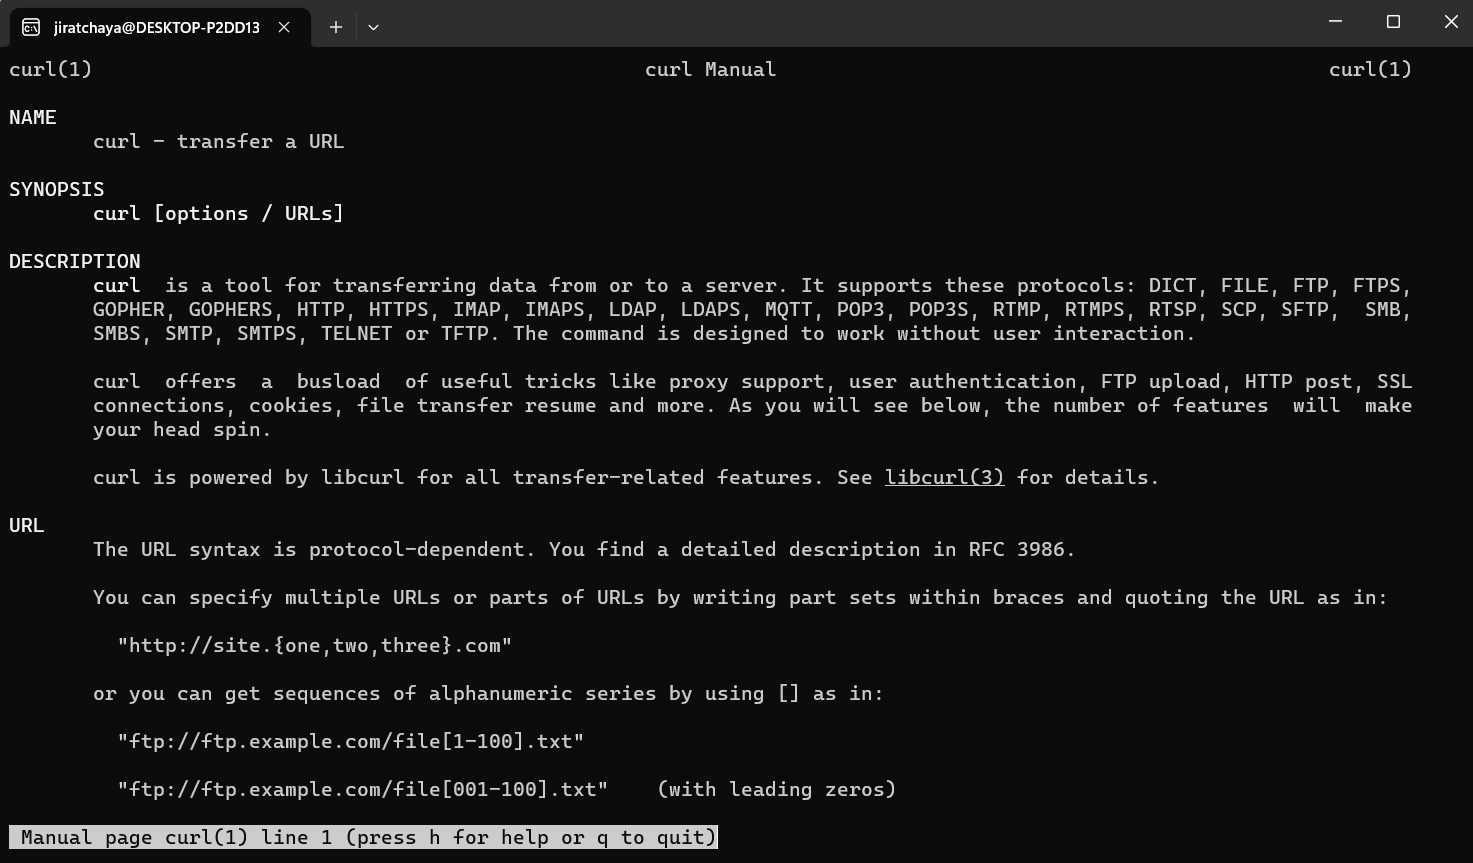
\includegraphics[width=0.8\textwidth,height=\textheight]{./assets/18_man_curl.png}

}

\caption{A manual page of \texttt{curl}. Users can scroll using arrow
keys up and down, and quit reading by press \texttt{q}.}

\end{figure}

\hypertarget{maintaining-long-running-jobs-with-tmux}{%
\section{Maintaining Long-Running Jobs with
tmux}\label{maintaining-long-running-jobs-with-tmux}}

When we run programs through the Unix shell, they run until they
terminate successfully or are terminated with an error. Multiple
processes running simultaneously on your computer, such as system files,
web browser, email application, bioinformatics programs, and so on. In
bioinformatics, we often work with processes that run for a long period
of time. Therefore, it's important that we know how to work with
processes and manage them using the Unix shell. In this section, we'll
learn the basics of dealing with processes.

In addition, processes are also terminated if the connection to the
servers is interrupted, the network connection drops immediately, or the
power fails. Since we're constantly working with remote computers in our
daily work in bioinformatics, we need a way to prevent the accidental
termination of long-running applications. Leaving the local terminal's
connection to a remote computer open while a program is running is an
unsafe solution, even the most reliable networks can experience short
outages.

\begin{figure}

{\centering \includegraphics{https://external-preview.redd.it/qevOpeiiyII34yThEPkMRIg6vL72zz-gt-zdQrfd-Us.jpg?auto=webp\&v=enabled\&s=e65d4473b8702e6437d5067d88f64d31a9822f51}

}

\caption{How tmux increase you pruductivity :/}

\end{figure}

Some software offers the user the possibility to run their work as a
background process, e.g.~Nohup, Screen and Tmux. In this workshop, we
propose \textbf{Terminal Multiplexer (Tmux)}, which allows you to create
a session with multiple windows, each of which can run its own
processes. The Tmux sessions are persistent, which means that all the
windows and their processes can be easily restored by reattaching the
session.

When Tmux is running on a remote machine, you can maintain a persistent
session that isn't lost when the connection drops or you close your
terminal window to go home (or even exit your terminal programme).
Rather, all Tmux sessions can be reattached to the terminal you're
currently at - simply log back into the remote machine via SSH and
reattach the Tmux session. All windows remain undisturbed and all
processes continue to run.

\hypertarget{a-simple-usage-of-tmux}{%
\subsection*{A simple usage of Tmux}\label{a-simple-usage-of-tmux}}
\addcontentsline{toc}{subsection}{A simple usage of Tmux}

Open a terminal and use the following command

\begin{Shaded}
\begin{Highlighting}[]
\ExtensionTok{tmux}
\end{Highlighting}
\end{Shaded}

You see a command prompt as usual, but you now see a taskbar-style menu
at the bottom of the terminal that contains something like bash 0 *. The
asterisk indicates that this is your active window.

\begin{figure}

{\centering 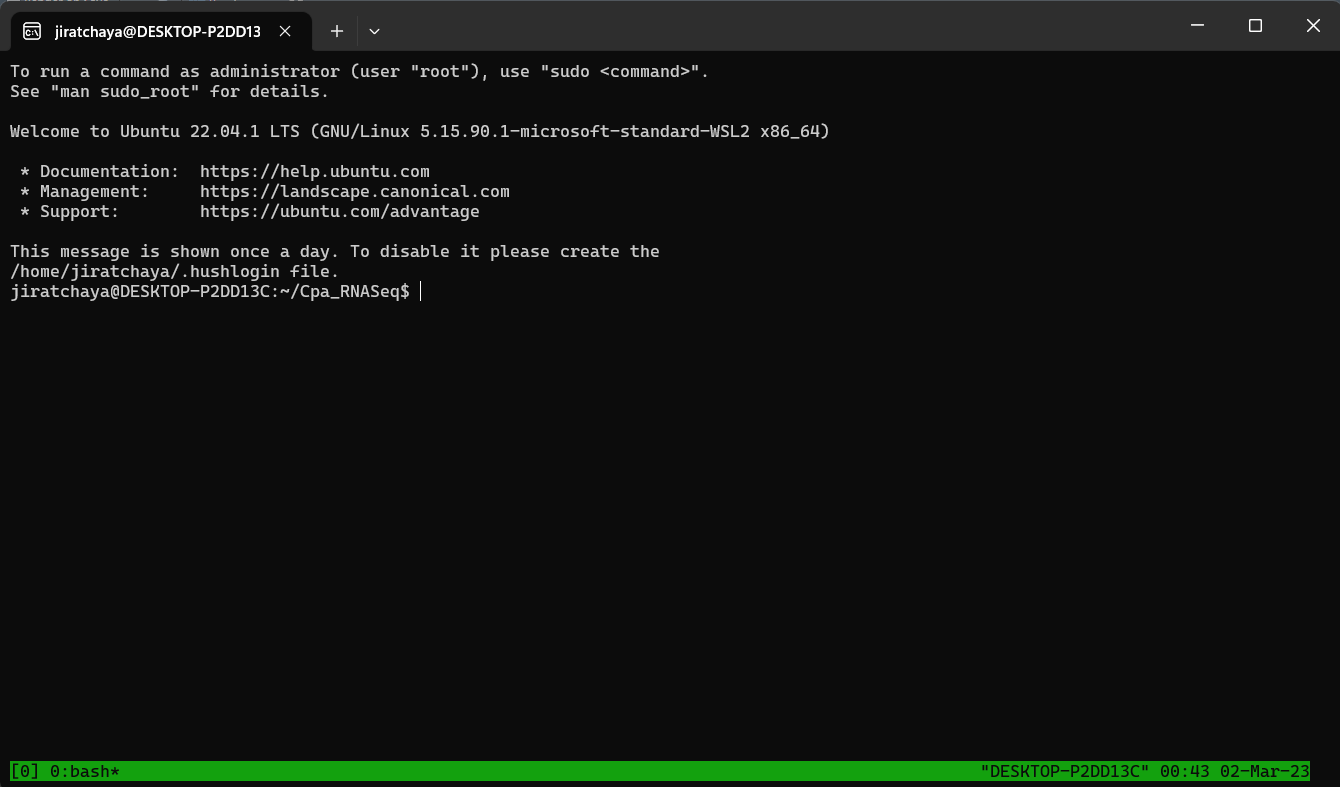
\includegraphics{./assets/10_tmux_simple.png}

}

\caption{Tmux windows}

\end{figure}

\hypertarget{detach-a-session}{%
\subsection*{Detach a session}\label{detach-a-session}}
\addcontentsline{toc}{subsection}{Detach a session}

This allows you to leave the tmux session, but it continues to run in
the background. Just press the key

\begin{verbatim}
[ctrl + b] + d
\end{verbatim}

Your terminal will print

\begin{verbatim}
jiratchaya@DESKTOP-P2DD13C:~/Cpa_RNASeq$ tmux
[detached (from session 0)]
\end{verbatim}

This should take you back to a standard prompt. Remember that the Tmux
session continues in the background, and you can recall it at any time.

\hypertarget{name-the-tmux-session}{%
\subsection*{Name the Tmux session}\label{name-the-tmux-session}}
\addcontentsline{toc}{subsection}{Name the Tmux session}

You may find it helpful to name your sessions with meaningful titles to
keep things organized. Let's try naming your first session with Tmux.

You can name it anything that we want, but in this case I will name it
`process2'. Enter the following command:

\begin{Shaded}
\begin{Highlighting}[]
\ExtensionTok{tmux}\NormalTok{ new }\AttributeTok{{-}s}\NormalTok{ process2}
\end{Highlighting}
\end{Shaded}

You should now have a new Tmux session running. If you look in the lower
left area of the window, you will see the name of your session rather
than the generic `bash'.

\hypertarget{list-tmux-sessions}{%
\subsection*{List tmux sessions}\label{list-tmux-sessions}}
\addcontentsline{toc}{subsection}{List tmux sessions}

What happened to your session? It is still running in the background.
You can reopen the session by name or number ID, but what if you forgot
the session name?

There is a list function built into tmux:

\begin{Shaded}
\begin{Highlighting}[]
\ExtensionTok{tmux}\NormalTok{ ls}
\end{Highlighting}
\end{Shaded}

This lists all your current tmux sessions. When you run it, you get
output like this:

\begin{figure}

{\centering 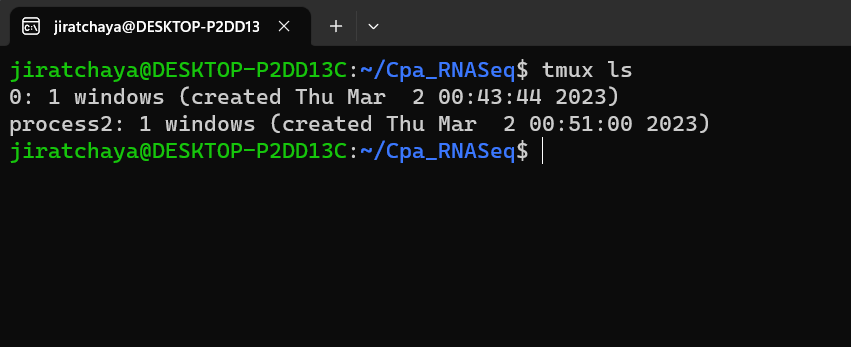
\includegraphics[width=0.75\textwidth,height=\textheight]{./assets/11_tmux_sessions.png}

}

\caption{List of running tmux sessions.}

\end{figure}

\hypertarget{reenter-aka-reattach-a-session-in-tmux}{%
\subsection*{Reenter (aka reattach) a session in
Tmux}\label{reenter-aka-reattach-a-session-in-tmux}}
\addcontentsline{toc}{subsection}{Reenter (aka reattach) a session in
Tmux}

To reopen your tmux session, you can use the tmux command with the
attach or attach-session option as follows:

\begin{verbatim}
tmux a -t [session_name]
\end{verbatim}

For example, we'll reenter to the process2 session.

\begin{Shaded}
\begin{Highlighting}[]
\ExtensionTok{tmux}\NormalTok{ a }\AttributeTok{{-}t}\NormalTok{ process2}
\end{Highlighting}
\end{Shaded}

\hypertarget{exit-tmux-when-finish-running}{%
\subsection*{Exit tmux when finish
running}\label{exit-tmux-when-finish-running}}
\addcontentsline{toc}{subsection}{Exit tmux when finish running}

Quitting tmux is exactly the same as quitting the standard terminal by
pressing the keys \texttt{Ctrl+d} or by entering

\begin{Shaded}
\begin{Highlighting}[]
\BuiltInTok{exit}
\end{Highlighting}
\end{Shaded}

\hypertarget{resources}{%
\section{Resources}\label{resources}}

\begin{itemize}
\item
  Buffalo, V. (2015).
  \href{https://books.google.co.th/books/about/Bioinformatics_Data_Skills.html?id=XxERCgAAQBAJ}{\emph{Bioinformatics
  data skills: Reproducible and robust research with open source
  tools}}. '' O'Reilly Media, Inc.''.
\item
  \href{https://hbctraining.github.io/Intro-to-shell-flipped/}{Introduction
  to the command line interface} by Harvard Chan Bioinformatics Core
  (Accessed on 27 Feb 2023).
\item
  \href{https://bioinformatics-core-shared-training.github.io/shell-genomics/01-introduction/index.html}{Introducing
  the Shell}, from the course Introduction to the Command Line for
  Genomics in bioinformatics-core-shared-training (Accessed on 28 Feb
  2023)
\item
  \href{https://github.com/RehanSaeed/Bash-Cheat-Sheet}{Bash cheat
  sheet} from RehanSaeed GitHub repository (Accessed on 1 March 2023).
\item
  \href{https://linuxhandbook.com/tmux/}{Getting Started with Tmux
  {[}Beginner's Guide{]}}. By linuxhandbook.com (Accessed on 2 March
  2023)
\end{itemize}

\bookmarksetup{startatroot}

\hypertarget{data-retrieval-with-ncbi-sra-toolkit}{%
\chapter{Data Retrieval with NCBI SRA
Toolkit}\label{data-retrieval-with-ncbi-sra-toolkit}}

NCBI (Natianal Center for Biotechnology Information) is a major source
of biological databases related to life and health sciences research, as
well as a major source of bioinformatics tools and services. NCBI hosts
various types of biological data submitted by researchers from around
the world, such as \href{https://www.ncbi.nlm.nih.gov/nuccore}{GenBank}
for nucleotide sequence submissions,
\href{https://www.ncbi.nlm.nih.gov/sra/}{Sequence Read Archive (SRA)}
for raw sequence data,
\href{https://www.ncbi.nlm.nih.gov/genome/}{Genome} for submitting full
or draft genomes, \href{https://www.ncbi.nlm.nih.gov/gds}{Gene
Expression Omnibus (GEO)} for quantitative gene expression data sets,
and many more.

\href{https://github.com/ncbi/sra-tools}{NCBI SRA toolkit} is a set of
utilities for downloading, viewing, and searching large amounts of
high-throughput sequencing data from the NCBI SRA database.

SRA toolkit can

\begin{itemize}
\tightlist
\item
  Effectively download the large volume of high-throughput sequencing
  data
\item
  Convert SRA file into other biological file format
\item
  Retrieve a small subset of large files
\item
  Search within SRA files and fetch specific sequences
\end{itemize}

\begin{figure}

{\centering \includegraphics[width=0.8\textwidth,height=\textheight]{https://i0.wp.com/ncbiinsights.ncbi.nlm.nih.gov/wp-content/uploads/2015/12/post-1-fig-1-toolkit-dls.png?resize=735\%252C660\&ssl=1}

}

\caption{Screenshots of NCBI Sequence Read Archives}

\end{figure}

\hypertarget{what-is-sequence-read-archives-sra}{%
\section{What is Sequence Read Archives
(SRA)}\label{what-is-sequence-read-archives-sra}}

The Sequence Read Archive (SRA) is the largest publicly accessible
repository for high-throughput sequencing data. SRA accepts data from
all areas of sequencing projects as well as metagenomics and
environmental studies. Sequencing data may be isolated from a single
species or from multiple species as in metagnomics studies.

SRA also refers in the file description to the format defined by NCBI
for NGS data in the SRA database. All data submitted to NCBI must be
stored in SRA format and can be converted back to a FASTQ, FASTA, or BAM
file depending on the original submission by the researchers. Here, the
SRA Toolkit provides tools for downloading data, converting various data
formats to SRA format and vice versa, and extracting SRA data to other
formats.

Researchers often use SRA data to make discoveries and conduct
reproducible research. Data sets can be compared using the SRA web
interface. However, if you want to download files for local use on your
computer, you should use a command line interface, and the SRA Toolkit
is highly recommended by NCBI.

\hypertarget{searching-rna-sequencing-datasets-in-ncbi}{%
\section{Searching RNA-Sequencing datasets in
NCBI}\label{searching-rna-sequencing-datasets-in-ncbi}}

The databases in NCBI are linked by some common features. This means
that you can start wherever you have your research problems in NCBI. In
this workshop, we will investigate transcriptional changes during light
exposure of the alga \emph{Cyanophora paradoxa}, a representative
species of Glaucophytes. For more information about this alga, please
see \href{https://www.science.org/doi/10.1126/science.1213561}{this
article in Science}.

\begin{tcolorbox}[enhanced jigsaw, breakable, bottomrule=.15mm, left=2mm, coltitle=black, opacityback=0, colframe=quarto-callout-note-color-frame, toprule=.15mm, opacitybacktitle=0.6, colbacktitle=quarto-callout-note-color!10!white, bottomtitle=1mm, colback=white, toptitle=1mm, titlerule=0mm, rightrule=.15mm, arc=.35mm, title=\textcolor{quarto-callout-note-color}{\faInfo}\hspace{0.5em}{Activity}, leftrule=.75mm]

You can easily search the SRA database for any keywords of interest
related to your research. In this context, we search for all SRA studies
related to \emph{C. paradoxa} and see what SRA provides us. Note that
the SRA database contains not only transcriptome studies, but also
genomes and metagenomes.

\begin{enumerate}
\def\labelenumi{\arabic{enumi}.}
\tightlist
\item
  Go to SRA database: \url{https://www.ncbi.nlm.nih.gov/sra}, and search
  for `cyanophora paradoxa'.
\end{enumerate}

\begin{figure}[H]

{\centering 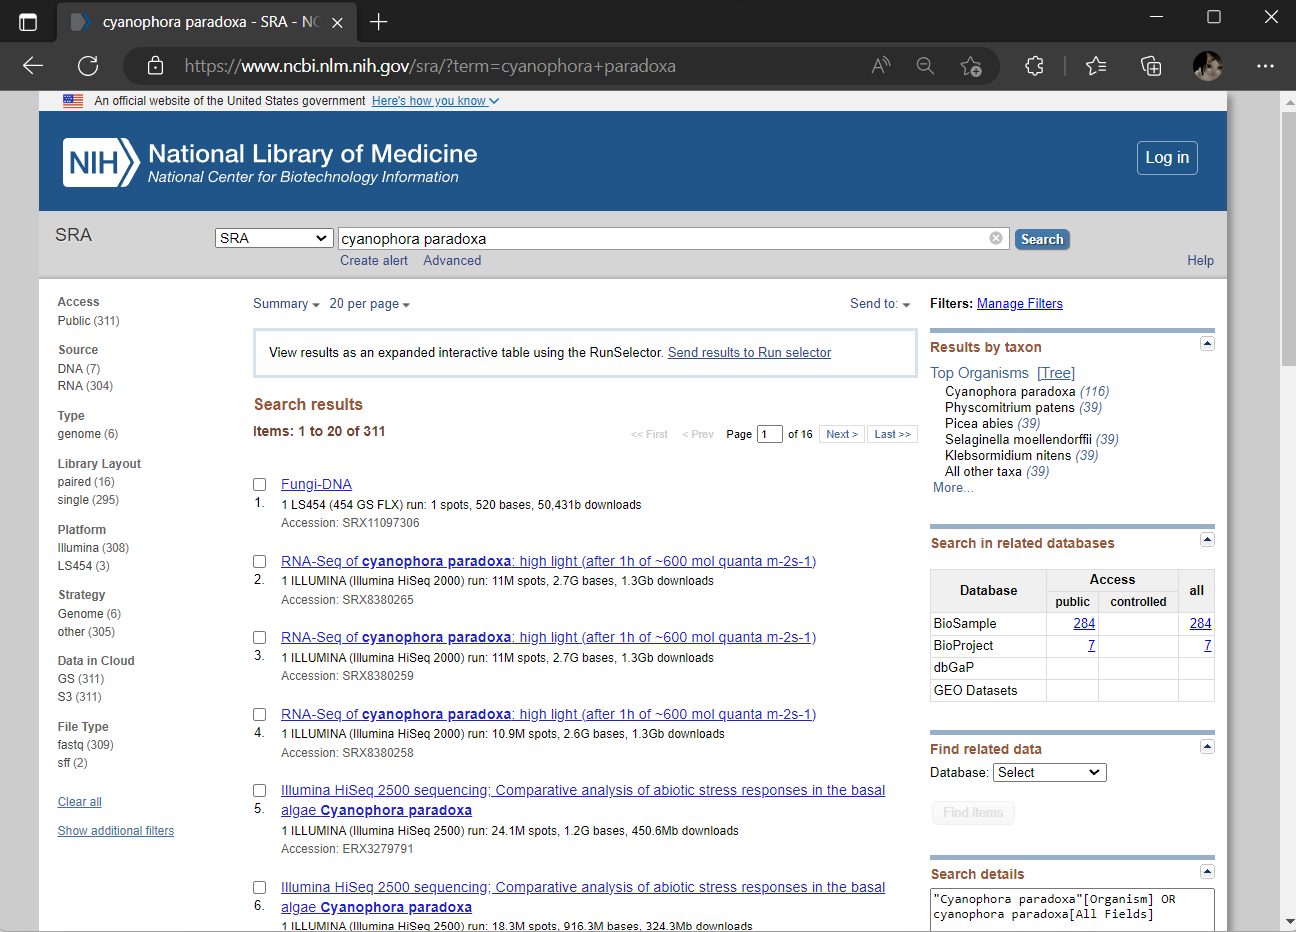
\includegraphics{./assets/14_ncbi_sra.png}

}

\caption{Screenshot of the search result of \emph{C. paradoxa} in the
database NCBI SRA. Here you can see all sequencing libraries of this
species that have been submitted to NCBI. You can specify which items
are of interest or customize the search using the filter box on the left
and right sides of the screen.}

\end{figure}

\begin{enumerate}
\def\labelenumi{\arabic{enumi}.}
\setcounter{enumi}{1}
\tightlist
\item
  We'll adjust our selection using the tool in the SRA database, the
  \textbf{\emph{SRA Run Selector}}, as follows.
\end{enumerate}

\begin{figure}[H]

{\centering \includegraphics{./assets/15_run_selector.gif}

}

\caption{Browsing sequencing data in NCBI SRA database}

\end{figure}

\begin{enumerate}
\def\labelenumi{\arabic{enumi}.}
\setcounter{enumi}{2}
\tightlist
\item
  In the SRA Run Selector, you can customize the filters based on the
  metadata columns of all runs. In this case, we filter the SRA runs
  based on the assay type as RNA-Seq and select only paired-end
  sequencing data as follows.
\end{enumerate}

\begin{figure}[H]

{\centering \includegraphics{./assets/16_run_selector_filtering.gif}

}

\caption{Customizing filters in SRA Run Selector}

\end{figure}

\begin{enumerate}
\def\labelenumi{\arabic{enumi}.}
\setcounter{enumi}{3}
\tightlist
\item
  Then you can select which runs you want to download and perform
  analysis. In this workshop we'll select \emph{C. paradoxa} RNA-Seq
  reads from \textbf{SRR8306028}, \textbf{SRR8306029},
  \textbf{SRR8306032}, \textbf{SRR8306033}, \textbf{SRR8306034} and
  \textbf{SRR8306035}.
\end{enumerate}

\begin{figure}[H]

{\centering \includegraphics{./assets/17_export_metadata.gif}

}

\caption{Exporting the selected metadata in SRA Run Selector.}

\end{figure}

\begin{enumerate}
\def\labelenumi{\arabic{enumi}.}
\setcounter{enumi}{4}
\tightlist
\item
  The downloaded metadata is in comma-separated file format. So you can
  open them with spreadsheet programs like Microsoft Excel on your local
  laptop. The metadata looks like this.
\end{enumerate}

\begin{table}
\centering\begingroup\fontsize{11}{13}\selectfont

\begin{tabular}{l|l|r|r|l|r|l|l|l|l|l|l|l|l|l|l|l|l|l|l|l|r|l|l|l|l|l|l|l|l|l|l|l|l|l|l|l|l|l|l|l|l|l|l|l|l|l|l|l|l|l|l|l|l|l|l|l|l|l|l|l|l|l|l|l|l|l|l|l}
\hline
Run & Assay.Type & AvgSpotLen & Bases & BioSample & Bytes & Center.Name & Consent & DATASTORE.filetype & DATASTORE.provider & DATASTORE.region & Experiment & Instrument & Library.Name & LibraryLayout & LibrarySelection & LibrarySource & Organism & Platform & ReleaseDate & create\_date & version & Sample.Name & SRA.Study & BioProject & ENA.FIRST.PUBLIC..run. & ENA\_first\_public & ENA.LAST.UPDATE..run. & ENA.LAST.UPDATE & External\_Id & INSDC\_center\_alias & INSDC\_center\_name & INSDC\_first\_public & INSDC\_last\_update & INSDC\_status & Sample\_Name & Submitter\_Id & Broker\_name & Developmental\_stage & Experimental\_Factor.\_stimulus..exp. & Genotype & growth\_condition & Organism\_part & stimulus & Experimental\_Factor.\_organism..exp. & Experimental\_Factor.\_time..exp. & Experimental\_Factor.\_growth\_condition..exp. & common\_name & BioSampleModel & geo\_loc\_name\_country & geo\_loc\_name\_country\_continent & geo\_loc\_name & Isolate & TISSUE & Collection\_Date & Isolation\_source & BIOMATERIAL\_PROVIDER & dev\_stage & Temp & TREATMENT & BREED & culture.collection & sequencer & source\_mat\_id & tissue\_type & Host & Lat\_Lon & Sample\_Type & Strain\\
\hline
SRR8306028 & RNA-Seq & 300 & 3373326900 & SAMN10588740 & 1950953927 & HHU DUESSELDORF & public & fastq,run.zq,sra & s3,ncbi,gs & gs.US,s3.us-east-1,ncbi.public & SRX5120515 & Illumina HiSeq 2000 & Cyanophora dark III & PAIRED & cDNA & TRANSCRIPTOMIC & Cyanophora paradoxa & ILLUMINA & 2019-08-05T00:00:00Z & 2018-12-17T16:48:00Z & 1 & Cyanophora\_dark & SRP173157 & PRJNA509798 & NA & NA & NA & NA & NA & NA & NA & NA & NA & NA & NA & NA & NA & NA & NA & NA & NA & NA & NA & NA & NA & NA & NA & Plant & Denmark & Europe & Denmark: obtained from the Scandinavian culture collection of Algae \& Protozoa (SCCAP) & SCCAP K-0262 & unicells & NA & NA & SCCAP K-0262 & exponential & 15 °C & 0 µmol quanta m-2s-1 & NA & NA & NA & NA & NA & NA & NA & NA & NA\\
\hline
SRR8306029 & RNA-Seq & 300 & 3361510200 & SAMN10588740 & 1882426113 & HHU DUESSELDORF & public & run.zq,fastq,sra & s3,ncbi,gs & gs.US,s3.us-east-1,ncbi.public & SRX5120514 & Illumina HiSeq 2000 & Cyanophora dark II & PAIRED & cDNA & TRANSCRIPTOMIC & Cyanophora paradoxa & ILLUMINA & 2019-08-05T00:00:00Z & 2018-12-17T16:44:00Z & 1 & Cyanophora\_dark & SRP173157 & PRJNA509798 & NA & NA & NA & NA & NA & NA & NA & NA & NA & NA & NA & NA & NA & NA & NA & NA & NA & NA & NA & NA & NA & NA & NA & Plant & Denmark & Europe & Denmark: obtained from the Scandinavian culture collection of Algae \& Protozoa (SCCAP) & SCCAP K-0262 & unicells & NA & NA & SCCAP K-0262 & exponential & 15 °C & 0 µmol quanta m-2s-1 & NA & NA & NA & NA & NA & NA & NA & NA & NA\\
\hline
SRR8306032 & RNA-Seq & 300 & 3378668400 & SAMN10588739 & 1903910409 & HHU DUESSELDORF & public & sra,run.zq,fastq & gs,s3,ncbi & ncbi.public,gs.US,s3.us-east-1 & SRX5120511 & Illumina HiSeq 2000 & Cyanophora light II & PAIRED & cDNA & TRANSCRIPTOMIC & Cyanophora paradoxa & ILLUMINA & 2019-08-05T00:00:00Z & 2018-12-17T16:44:00Z & 1 & Cyanophora\_normal light & SRP173157 & PRJNA509798 & NA & NA & NA & NA & NA & NA & NA & NA & NA & NA & NA & NA & NA & NA & NA & NA & NA & NA & NA & NA & NA & NA & NA & Plant & Denmark & Europe & Denmark: obtained from the Scandinavian culture collection of Algae \& Protozoa (SCCAP) & SCCAP K-0262 & unicells & NA & NA & SCCAP K-0262 & exponential & 15 °C & \textasciitilde{} 50 µmol quanta m-2s-1 & NA & NA & NA & NA & NA & NA & NA & NA & NA\\
\hline
SRR8306033 & RNA-Seq & 300 & 3386020200 & SAMN10588739 & 1892499340 & HHU DUESSELDORF & public & fastq,run.zq,sra & ncbi,s3,gs & gs.US,ncbi.public,s3.us-east-1 & SRX5120510 & Illumina HiSeq 2000 & Cyanophora light I & PAIRED & cDNA & TRANSCRIPTOMIC & Cyanophora paradoxa & ILLUMINA & 2019-08-05T00:00:00Z & 2018-12-17T16:35:00Z & 1 & Cyanophora\_normal light & SRP173157 & PRJNA509798 & NA & NA & NA & NA & NA & NA & NA & NA & NA & NA & NA & NA & NA & NA & NA & NA & NA & NA & NA & NA & NA & NA & NA & Plant & Denmark & Europe & Denmark: obtained from the Scandinavian culture collection of Algae \& Protozoa (SCCAP) & SCCAP K-0262 & unicells & NA & NA & SCCAP K-0262 & exponential & 15 °C & \textasciitilde{} 50 µmol quanta m-2s-1 & NA & NA & NA & NA & NA & NA & NA & NA & NA\\
\hline
SRR8306034 & RNA-Seq & 300 & 3436771500 & SAMN10588740 & 1902846665 & HHU DUESSELDORF & public & fastq,run.zq,sra & ncbi,s3,gs & gs.US,ncbi.public,s3.us-east-1 & SRX5120509 & Illumina HiSeq 2000 & Cyanophora dark I & PAIRED & cDNA & TRANSCRIPTOMIC & Cyanophora paradoxa & ILLUMINA & 2019-08-05T00:00:00Z & 2018-12-17T16:38:00Z & 1 & Cyanophora\_dark & SRP173157 & PRJNA509798 & NA & NA & NA & NA & NA & NA & NA & NA & NA & NA & NA & NA & NA & NA & NA & NA & NA & NA & NA & NA & NA & NA & NA & Plant & Denmark & Europe & Denmark: obtained from the Scandinavian culture collection of Algae \& Protozoa (SCCAP) & SCCAP K-0262 & unicells & NA & NA & SCCAP K-0262 & exponential & 15 °C & 0 µmol quanta m-2s-1 & NA & NA & NA & NA & NA & NA & NA & NA & NA\\
\hline
SRR8306035 & RNA-Seq & 300 & 3436308000 & SAMN10588739 & 1909811743 & HHU DUESSELDORF & public & run.zq,fastq,sra & s3,gs,ncbi & gs.US,s3.us-east-1,ncbi.public & SRX5120508 & Illumina HiSeq 2000 & Cyanophora light III & PAIRED & cDNA & TRANSCRIPTOMIC & Cyanophora paradoxa & ILLUMINA & 2019-08-05T00:00:00Z & 2018-12-17T15:00:00Z & 1 & Cyanophora\_normal light & SRP173157 & PRJNA509798 & NA & NA & NA & NA & NA & NA & NA & NA & NA & NA & NA & NA & NA & NA & NA & NA & NA & NA & NA & NA & NA & NA & NA & Plant & Denmark & Europe & Denmark: obtained from the Scandinavian culture collection of Algae \& Protozoa (SCCAP) & SCCAP K-0262 & unicells & NA & NA & SCCAP K-0262 & exponential & 15 °C & \textasciitilde{} 50 µmol quanta m-2s-1 & NA & NA & NA & NA & NA & NA & NA & NA & NA\\
\hline
\end{tabular}
\endgroup{}
\end{table}

\end{tcolorbox}

\hypertarget{downloading-sra-runs-using-fasterq-dump}{%
\section{\texorpdfstring{Downloading SRA runs using
\emph{fasterq-dump}}{Downloading SRA runs using fasterq-dump}}\label{downloading-sra-runs-using-fasterq-dump}}

\texttt{fasterq-dump} are tools in the SRA toolkit used to connect from
our remote server to the NCBI server and download sequencing data from
SRA.

According to the
\href{https://github.com/ncbi/sra-tools/wiki/08.-prefetch-and-fasterq-dump\#how-to-use-prefetch-and-fasterq-dump-to-extract-fastq-files-from-sra-accessions}{NCBI
sra-tools' guideline}, using \texttt{fasterq-dump} in combination with
another tool, \texttt{prefetch}, is the better way to download data
because \texttt{prefetch} can be invoked at any time if the previous
download accidentally failed. So it is not necessary to start the
download from the beginning.

However, \texttt{prefetch} can sometimes be skipped if you want to
download a small amount of data. In this workshop we'll use only
\texttt{fasterq-dump} to download and process SRA file format to FASTQ
file for further analysis.

\begin{tcolorbox}[enhanced jigsaw, breakable, bottomrule=.15mm, left=2mm, coltitle=black, opacityback=0, colframe=quarto-callout-note-color-frame, toprule=.15mm, opacitybacktitle=0.6, colbacktitle=quarto-callout-note-color!10!white, bottomtitle=1mm, colback=white, toptitle=1mm, titlerule=0mm, rightrule=.15mm, arc=.35mm, title=\textcolor{quarto-callout-note-color}{\faInfo}\hspace{0.5em}{Activity}, leftrule=.75mm]

We'll do the following command in Terminal or MobaXterm, by access to
the username and password that we've provided.

\begin{itemize}
\item
  For mobaXterm, enter to your session.
\item
  For terminal, type
\end{itemize}

\begin{Shaded}
\begin{Highlighting}[]
\FunctionTok{ssh} \OperatorTok{\textless{}}\NormalTok{username}\OperatorTok{\textgreater{}}\NormalTok{@}\OperatorTok{\textless{}}\NormalTok{server IP address}\OperatorTok{\textgreater{}}
\end{Highlighting}
\end{Shaded}

Now we download RNA-Seq libraries from \emph{C. paradoxa} using the SRA
accessions listed in the first column of the metadata above using the
following command.

Activate analysis environment

\begin{Shaded}
\begin{Highlighting}[]
\ExtensionTok{conda}\NormalTok{ activate ncbi}
\end{Highlighting}
\end{Shaded}

Go to working directory

\begin{Shaded}
\begin{Highlighting}[]
\BuiltInTok{cd}\NormalTok{ \textasciitilde{}/Cpa\_RNASeq/01\_Rawdata}
\end{Highlighting}
\end{Shaded}

Run fasterq-dump

\begin{Shaded}
\begin{Highlighting}[]
\ExtensionTok{fasterq{-}dump} \AttributeTok{{-}{-}threads}\NormalTok{ 2 }\AttributeTok{{-}{-}progress} \DataTypeTok{\textbackslash{}}
\NormalTok{SRR8306028 SRR8306029 SRR8306032 }\DataTypeTok{\textbackslash{}}
\NormalTok{SRR8306033 SRR8306034 SRR8306035}
\end{Highlighting}
\end{Shaded}

From the \texttt{fasterq-dump} command,

\texttt{-\/-threads} refer to how many threads to use (default = 6).

\texttt{-\/-progress} force the terminal to print the progress of
downloading and processing file to the screen.

Expected output files.

\begin{verbatim}
01_Rawdata
├── SRR8306028_1.fastq
├── SRR8306028_2.fastq
├── SRR8306029_1.fastq
├── SRR8306029_2.fastq
├── SRR8306032_1.fastq
├── SRR8306032_2.fastq
├── SRR8306033_1.fastq
├── SRR8306033_2.fastq
├── SRR8306034_1.fastq
├── SRR8306034_2.fastq
├── SRR8306035_1.fastq
└── SRR8306035_2.fastq
\end{verbatim}

\end{tcolorbox}

By default, \texttt{fasterq-dump} processes a single SRA file format of
paired-end reads by splitting reads into forward (\texttt{*\_1.fastq})
and reverse (\texttt{*\_2.fastq}), if singletons (unpaired between
forward and reverse reads) present, it will be written to another fastq
file as described in this figure.

\begin{figure}

{\centering \includegraphics[width=0.8\textwidth,height=\textheight]{https://github.com/ncbi/sra-tools/wiki/images/split3-mode.png}

}

\caption{Sequence read processing by fasterq-dump using default
parameters. Figure adopted from
\url{https://github.com/ncbi/sra-tools/wiki/HowTo:-fasterq-dump}.}

\end{figure}

\hypertarget{reference-sources}{%
\section{Reference Sources}\label{reference-sources}}

\begin{itemize}
\tightlist
\item
  Price, Dana C., et al.~``\emph{Cyanophora paradoxa} genome elucidates
  origin of photosynthesis in algae and plants.'' \emph{Science}
  335.6070 (2012): 843-847.
  \url{https://doi.org/10.1126/science.1213561}.
\item
  \href{https://ncbiinsights.ncbi.nlm.nih.gov/2015/12/11/sra-toolkit-the-sra-database-at-your-fingertips/}{SRA
  Toolkit: the SRA database at your fingertips} from NCBI Insights.
  Accessed 4-Mar-2023.
\item
  \href{https://www.reneshbedre.com/blog/ncbi_sra_toolkit.html}{How to
  use NCBI SRA Toolkit effectively} by Renesh Bedre, Data science blog.
  Accessed 4-Mar-2023.
\item
  \href{https://github.com/ncbi/sra-tools/wiki/HowTo:-fasterq-dump}{HowTo:
  fasterq dump} by NCBI sra-tools GitHub Wiki. Accessed 4-Mar-2023.
\end{itemize}

\bookmarksetup{startatroot}

\hypertarget{rna-seq-data-quality-control}{%
\chapter{RNA-Seq Data Quality
Control}\label{rna-seq-data-quality-control}}

\hypertarget{what-is-fastq-file-format}{%
\section{What is FASTQ file format}\label{what-is-fastq-file-format}}

Next-generation sequencing and data analysis projects typically begin
with the processing of sequence read data and their quality tags from
the sequencer in FASTQ format. The FASTQ format is the most commonly
used format in sequence analysis and is generated by a sequencer. The
FASTQ file contains the sequence data from the clusters that pass the
filter of a flow cell. Many analysis tools require this format because
it contains much more information than FASTA. In this workshop, we will
mainly explain the FASTQ file format, which comes from the Illumina
sequencer.

The FASTQ format is similar to the fasta format, but differs in syntax
and in the integration of quality values. Each sequence requires at
least 4 lines:

\begin{figure}

{\centering 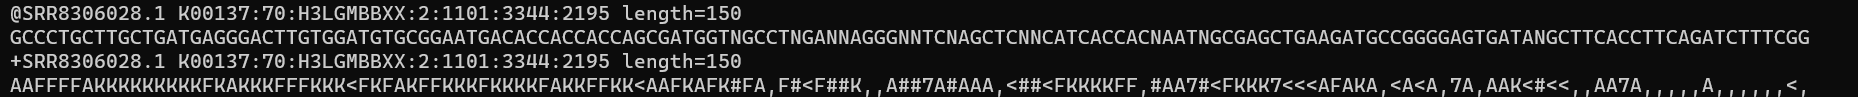
\includegraphics{assets/12_fastq_format.png}

}

\caption{Example of FASTQ file format}

\end{figure}

\begin{enumerate}
\def\labelenumi{\arabic{enumi}.}
\item
  A sequence identifier with information about the sequencing run and
  the cluster. The exact contents of this line vary by based on the BCL
  to FASTQ conversion software used.
\item
  The sequence (the base calls; A, C, T, G and N).
\item
  A separator, which is simply a plus (+) sign.
\item
  The base call quality scores. These are Phred +33 encoded, using ASCII
  characters to represent the numerical quality scores.
\end{enumerate}

The FastQ sequence descriptor generally follows a specific format that
includes all information about the sequencer and its position on the
flow cell. The sequence descriptor also follows a specific format and
contains information about the sample information.

FASTQ sequence descriptor, particulary in Illumina sequence reads look
like:

\begin{verbatim}
@HWUSI-EAS100R:6:73:941:1973#0/1
\end{verbatim}

where

\begin{longtable}[]{@{}
  >{\raggedright\arraybackslash}p{(\columnwidth - 2\tabcolsep) * \real{0.2159}}
  >{\raggedright\arraybackslash}p{(\columnwidth - 2\tabcolsep) * \real{0.7841}}@{}}
\toprule()
\endhead
\textbf{HWUSI-EAS100R} & The unique instrument name \\
\textbf{6} & Flowcell lane \\
\textbf{73} & Tile number within the flowcell lane \\
\textbf{941} & `x'-coordinate of the cluster within the tile \\
\textbf{1973} & `y'-coordinate of the cluster within the tile \\
\textbf{\#0} & Index number for a multiplexed sample (0 for no
indexing) \\
\textbf{/1} & The member of a pair, /1 or /2 (paired-end or mate-pair
reads only) \\
\bottomrule()
\end{longtable}

As mentioned earlier, line 4 contains the quality score of the
nucleotide at the same position. The quality scores are represented by
the code ASCII, which indicates how confident of the correctly called
base is.

We can calculate the quality score of a base,if P is the error
probability, then:

\[
\text{Q} = \text{-10}log_{10}\left( P \right)
\]

The following figure shows the representative ASCII code for the score
value. Base quality scoring for analysis is important when identifying
types of genomic variation such as SNPs, but it is also an indicator of
the overall quality of the sequencing as well.

\begin{figure}

{\centering \includegraphics{https://www.drive5.com/usearch/manual/qscores.gif}

}

\caption{Tables converting between integer Q scores, ASCII characters
and error probabilities. Figure adopted from
https://www.drive5.com/usearch/manual/quality\_score.html}

\end{figure}

\hypertarget{what-software-use-fastq}{%
\subsection{What software use FASTQ}\label{what-software-use-fastq}}

To date, Almost NGS analysis software requires FASTQ format. For
example:

\begin{itemize}
\item
  QC such as
  \href{https://www.bioinformatics.babraham.ac.uk/projects/fastqc/}{fastQC}
  used FASTQ to determine how good of the sequence read library,
  generate an informative report, and also determining the presence of
  adapter sequences which can also be trimmed by some integrated QC
  tools such as \href{https://github.com/OpenGene/fastp}{FASTP}.
\item
  Aligners such as
  \href{https://github.com/BenLangmead/bowtie2}{bowtie2},
  \href{https://github.com/lh3/bwa}{BWA},
  \href{https://github.com/alexdobin/STAR}{STAR}, and so on, use reads,
  and quality sometimes, to align to the reference sequence. The mapping
  information can be further used for quantifying expression,
  constructing sequence assembly, and variant calling.
\item
  De novo assembly tools, for example
  \href{https://github.com/trinityrnaseq/trinityrnaseq}{Trinity},
  \href{https://github.com/ablab/spades}{Spades},
  \href{https://github.com/dzerbino/velvet}{Velvet}, etc., also use
  FASTQ to construct contig library and scaffolding. Some de novo
  assembler tools not only use FASTQ to contruct draft assembly but also
  used in the polishing process to refine assembly, such as
  \href{https://github.com/fenderglass/Flye}{Flye},
  \href{https://github.com/rrwick/Unicycler}{Unicycler},
  \href{https://github.com/marbl/canu}{Canu}, etc.
\end{itemize}

\hypertarget{quality-assessment-using-fastqc}{%
\section{Quality assessment using
FastQC}\label{quality-assessment-using-fastqc}}

FastQC is designed for quality control of raw sequence data from
high-throughput sequencing technology. It provides a modular set of
analyses that you can use to get a quick overview of the quantity and
quality of your data, and to help you decide on the raw data whether you
should perform adapter or low-quality read trimming or whether you can
perform further analyses. For sequence reads that require adapter
trimming before further analysis, we recommended to assessing the
quality both before and after trimming.

Most sequencers will generate a QC report as part of their analysis
pipeline, but this is usually only focused on identifying problems which
were generated by the sequencer itself. FastQC aims to provide a QC
report which can spot problems which originate either in the sequencer
or in the starting library material.

\begin{tcolorbox}[enhanced jigsaw, breakable, bottomrule=.15mm, left=2mm, coltitle=black, opacityback=0, colframe=quarto-callout-note-color-frame, toprule=.15mm, opacitybacktitle=0.6, colbacktitle=quarto-callout-note-color!10!white, bottomtitle=1mm, colback=white, toptitle=1mm, titlerule=0mm, rightrule=.15mm, arc=.35mm, title=\textcolor{quarto-callout-note-color}{\faInfo}\hspace{0.5em}{Activity}, leftrule=.75mm]

The following will perform on you user account by activating your
working environment at first.

\begin{Shaded}
\begin{Highlighting}[]
\ExtensionTok{conda}\NormalTok{ activate qc}
\end{Highlighting}
\end{Shaded}

Then, create a directory for QC result before adapter trimming

\begin{Shaded}
\begin{Highlighting}[]
\FunctionTok{mkdir}\NormalTok{ 02\_QC/fastQC\_before\_trim}
\end{Highlighting}
\end{Shaded}

Run FastQC all file at once. Here, we'll use a wildcard \texttt{*.fastq}
to select all FASTQ files in 01\_Rawdata directory. We also specify
number of CPU threads in \texttt{-\/-threads} and QC output files in
02\_QC/fastQC\_before\_trim using \texttt{-\/-outdir} argument.

\begin{Shaded}
\begin{Highlighting}[]
\ExtensionTok{fastqc} \AttributeTok{{-}{-}outdir}\NormalTok{ 02\_QC/fastQC\_before\_trim }\DataTypeTok{\textbackslash{}}
\NormalTok{{-}{-}threads 2 }\DataTypeTok{\textbackslash{}}
\NormalTok{01\_Rawdata/}\PreprocessorTok{*}\NormalTok{.fastq}
\end{Highlighting}
\end{Shaded}

\end{tcolorbox}

\hypertarget{interpreting-fastqc-results}{%
\section{Interpreting FastQC
results}\label{interpreting-fastqc-results}}

FastQC also provided excellent explanation of each analysis step in
their documentation. So we encouraged you to learn more at their
\href{https://www.bioinformatics.babraham.ac.uk/projects/fastqc/}{web
page} along with the
\href{https://www.bioinformatics.babraham.ac.uk/projects/fastqc/Help/}{documentation}.

The analysis in FastQC is performed by a series of analysis modules. The
left hand side of the main interactive display or the top of the HTML
report show a summary of the modules which were run, and a quick
evaluation of whether the results of the module seem entirely normal
(green tick), slightly abnormal (orange triangle) or very unusual (red
cross).

\begin{figure}

{\centering 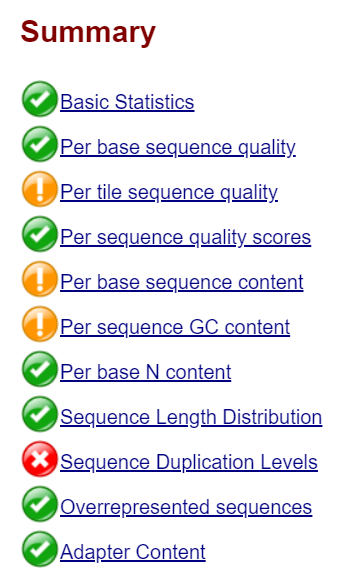
\includegraphics[width=0.3\textwidth,height=\textheight]{./assets/19_fqc_sidebar.png}

}

\caption{FastQC sidebar}

\end{figure}

\hypertarget{basic-statistics}{%
\subsection{Basic statistics}\label{basic-statistics}}

The Basic Statistics module generates some simple composition statistics
for the file analysed.

\begin{figure}

{\centering 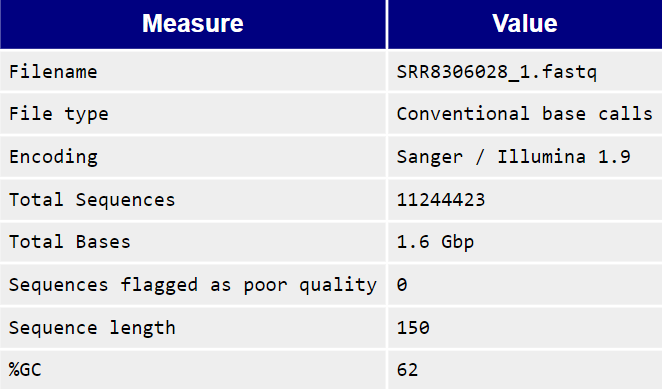
\includegraphics[width=0.5\textwidth,height=\textheight]{./assets/20_fqc_basic_stat.png}

}

\caption{Basic statistics of SRR8306028.}

\end{figure}

\begin{itemize}
\item
  \textbf{Filename:} The original filename of the file which was
  analysed
\item
  \textbf{File type:} Says whether the file appeared to contain actual
  base calls or colorspace data which had to be converted to base calls
\item
  \textbf{Encoding:} Says which ASCII encoding of quality values was
  found in this file.
\item
  \textbf{Total Sequences:} A count of the total number of sequences
  processed. There are two values reported, actual and estimated. At the
  moment these will always be the same. In the future it may be possible
  to analyse just a subset of sequences and estimate the total number,
  to speed up the analysis, but since we have found that problematic
  sequences are not evenly distributed through a file we have disabled
  this for now.
\item
  \textbf{Sequence Length:} Provides the length of the shortest and
  longest sequence in the set. If all sequences are the same length only
  one value is reported. \%GC: The overall \%GC of all bases in all
  sequences
\end{itemize}

\hypertarget{per-base-sequence-quality}{%
\subsection{Per Base Sequence Quality}\label{per-base-sequence-quality}}

The Per base sequence quality plot shows an overview of the range of
quality values across all bases at each position in the FastQ file.

\begin{figure}

{\centering 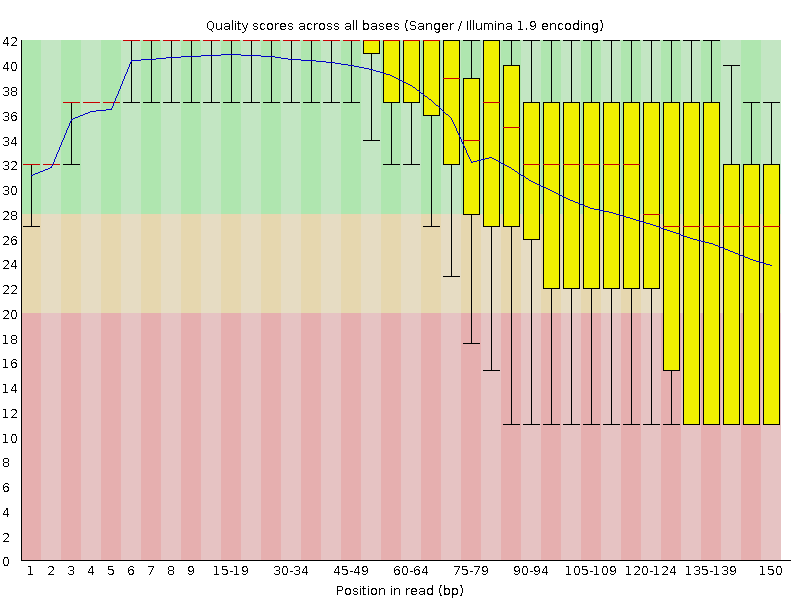
\includegraphics[width=0.7\textwidth,height=\textheight]{./assets/21_fqc_per_base_seq_qual.png}

}

\caption{Per Base Sequence Quality plot of SRR8306028. In which the
central red line is the median value. The yellow box represents the
inter-quartile range (25-75\%). The upper and lower whiskers represent
the 10\% and 90\% points. The blue line represents the mean quality.}

\end{figure}

The higher the score, the better the base call, i.e., the box plots fall
into the very good quality area (green background), the mediocre quality
area (orange background), and the poor quality area (red background).
The following figures show a comparison of the good and poor quality
results of Illumina sequencing technology.

\begin{figure}

{\centering 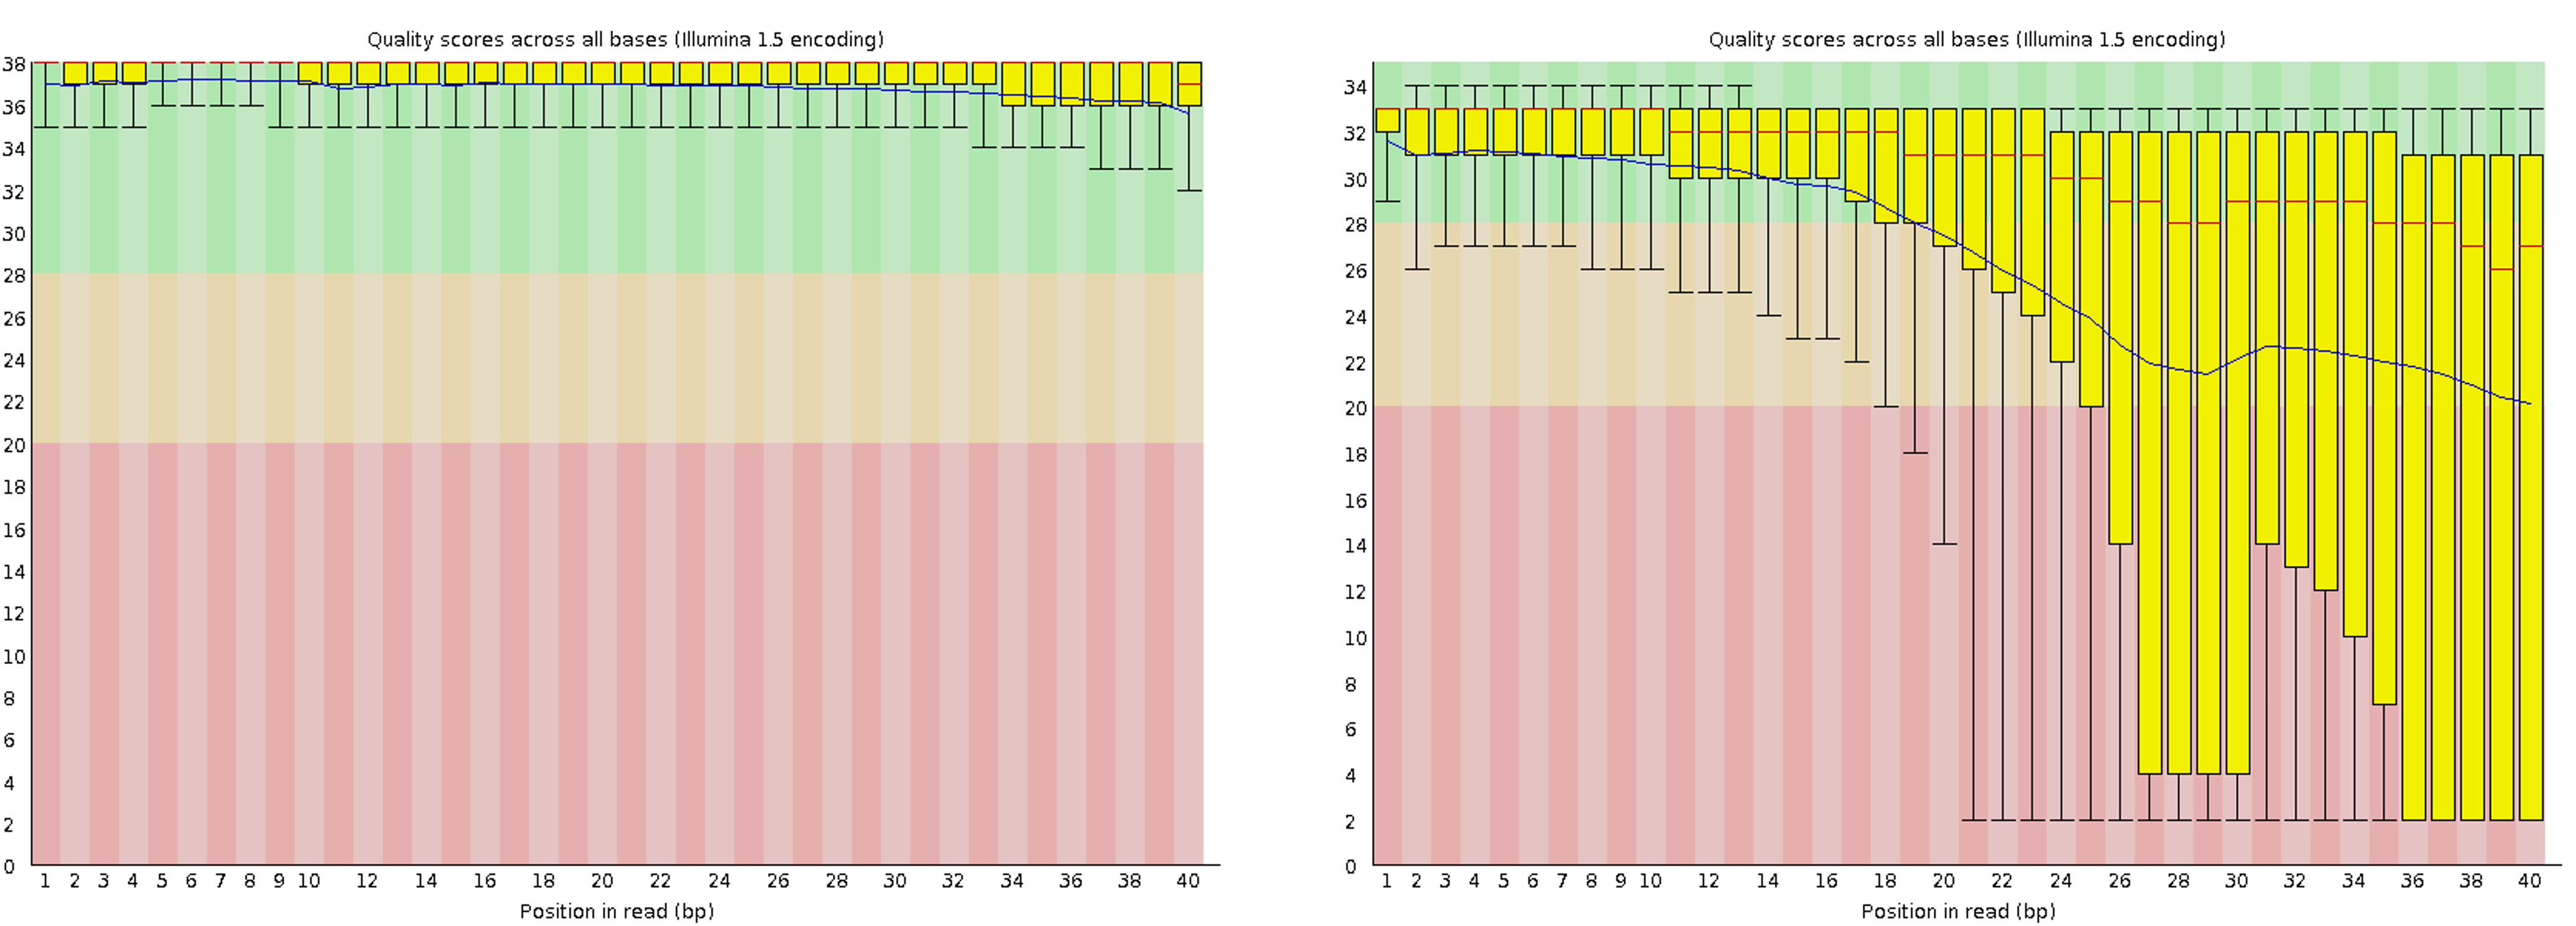
\includegraphics{./assets/31_fqc_compare_quality.png}

}

\caption{A comparison of good (left) and bad (right) per base sequence
quality plots. Figures adopted from example reports in
\url{https://www.bioinformatics.babraham.ac.uk/projects/fastqc}.}

\end{figure}

\hypertarget{per-tile-sequence-quality}{%
\subsection{Per tile sequence quality}\label{per-tile-sequence-quality}}

This plot is specific to Illumina sequencing libraries and shows colour
shading of quality score by position on the flow cell. The colours are
on a scale from cold to hot, with cold colours representing positions
where the quality was at or above average for that base in the run, and
hotter colours indicating that a tile had worse qualities than other
tiles for that base. In the example below, you can see that certain
tiles have consistently poor quality. A good chart should be blue
throughout.

\begin{figure}

{\centering 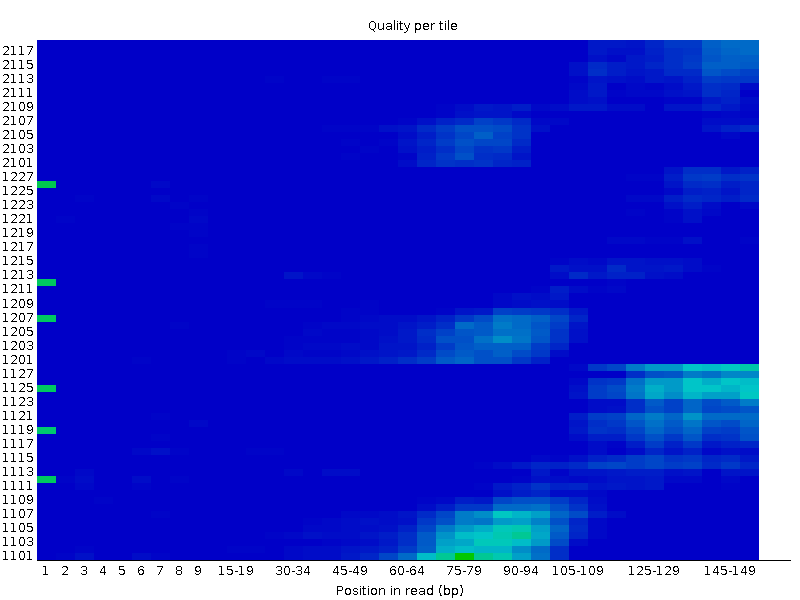
\includegraphics[width=0.7\textwidth,height=\textheight]{./assets/22_fqc_per_tile_seq_qual.png}

}

\caption{Per tile sequence quality plot of SRR8306028.}

\end{figure}

\hypertarget{per-sequence-quality-scores}{%
\subsection{Per Sequence Quality
Scores}\label{per-sequence-quality-scores}}

The per sequence quality score report allows you to see if a subset of
your sequences have universally low quality values. It is often the case
that a subset of sequences will have universally poor quality, often
because they are poorly imaged (on the edge of the field of view etc),
however these should represent only a small percentage of the total
sequences.

\begin{figure}

{\centering 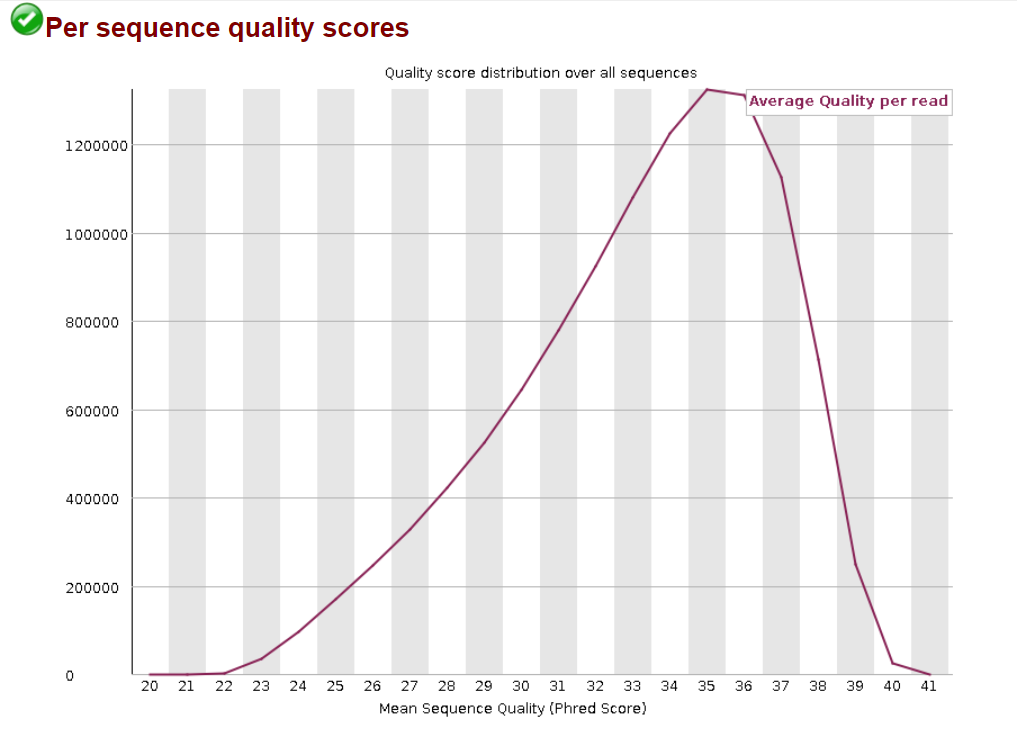
\includegraphics[width=0.7\textwidth,height=\textheight]{./assets/23_fqc_per_seq_qual.png}

}

\caption{Per Sequence Quality Scores plot of SRR8306028.}

\end{figure}

\hypertarget{per-base-sequence-content}{%
\subsection{Per Base Sequence Content}\label{per-base-sequence-content}}

Per Base Sequence Content plots out the proportion of each base position
in a file for which each of the four normal DNA bases has been called.
The plot shows the quality of nucleotide A T C and G separately into 4
lines.

\begin{figure}

{\centering 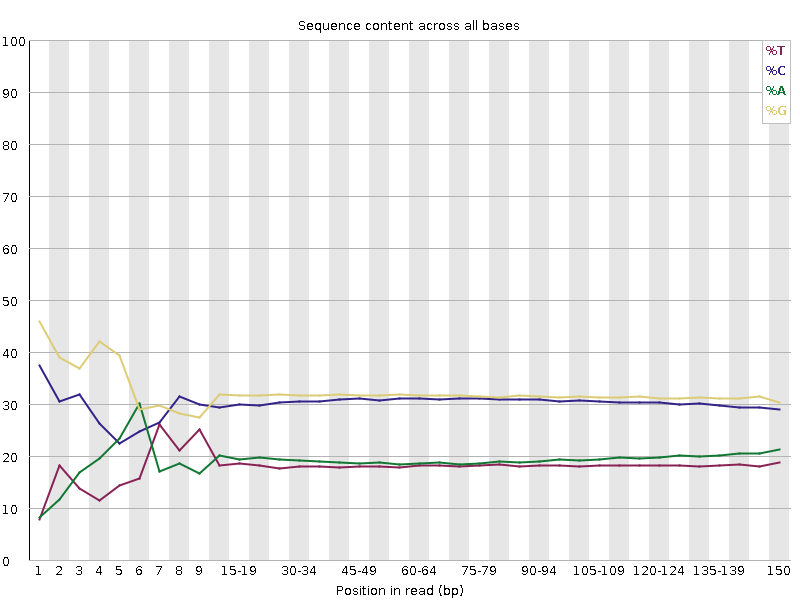
\includegraphics[width=0.7\textwidth,height=\textheight]{./assets/24_fqc_per_base_seq_content.png}

}

\caption{Per Base Sequence Content plot of SRR8306028.}

\end{figure}

Usually ambiguous base values are found at the beginning of the read.
Libraries made with random hexamer primers, with almost all RNA-Seq
libraries using them, and those that were fragmented libraries. This
bias does not affect an absolute sequence, but provides enrichment of a
number of different K-mers at the 5' end of the reads. While this is a
true technical bias, it cannot be corrected by trimming and does not
appear to affect downstream analysis in most cases. However, a warning
or error is generated in this module. This module issues a warning if
the difference between A and T, or G and C is greater than 10\% in any
position.

\hypertarget{per-sequence-gc-content}{%
\subsection{Per Sequence GC Content}\label{per-sequence-gc-content}}

This module measures the GC content over the entire length of each
sequence in a file and compares it to a normal distribution of GC
content. Normally, one would expect an approximately normal distribution
of GC content, where the central peak corresponds to the total GC
content of the underlying genome of interest.

The skewness of the distribution may indicate some unusual events such
as contamination or systematic bias in your sequencing library. However,
the GC content signature of different organisms may depend on their
nature.

\begin{figure}

{\centering 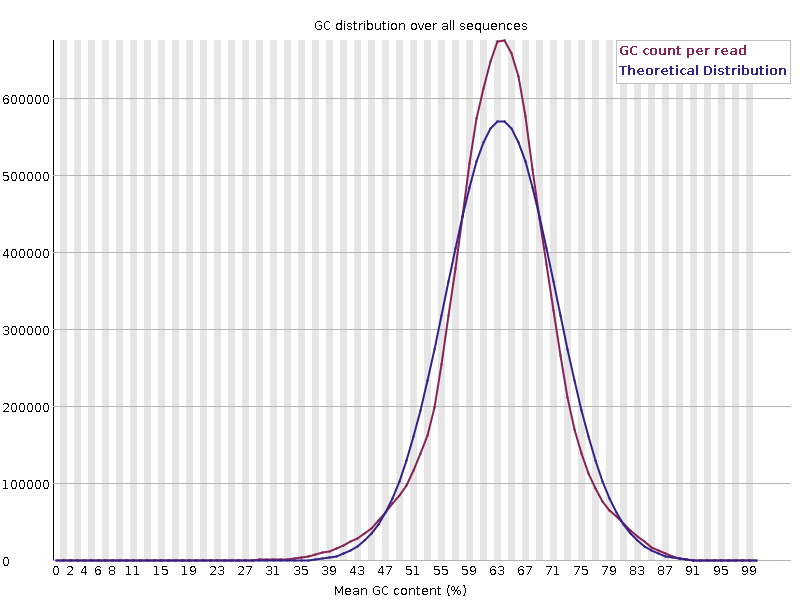
\includegraphics[width=0.7\textwidth,height=\textheight]{./assets/25_fqc_gc_content.png}

}

\caption{Per Sequence GC Content plot of SRR8306028.}

\end{figure}

\hypertarget{per-base-n-content}{%
\subsection{Per base N content}\label{per-base-n-content}}

This module represents the percentage of base calls at each position for
which an N was called. The `N' base is found when the sequencer is not
able to make a confident base call, then it will normally substitute an
N.

\begin{figure}

{\centering 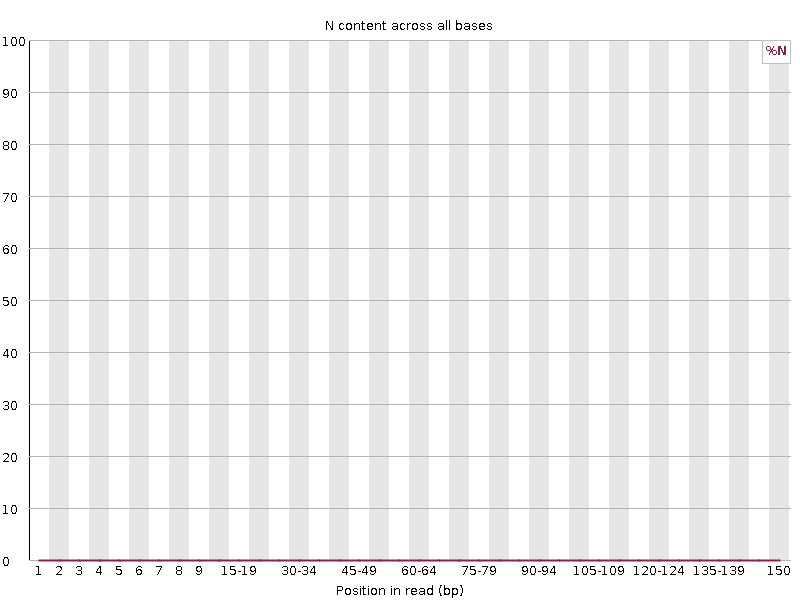
\includegraphics[width=0.7\textwidth,height=\textheight]{./assets/26_fqc_N.png}

}

\caption{Per base N content plot of SRR8306028.}

\end{figure}

\hypertarget{sequence-length-distribution}{%
\subsection{Sequence Length
Distribution}\label{sequence-length-distribution}}

This module generates a histogram of distribution of sequence reads in
the file which was analyzed.

\begin{figure}

{\centering 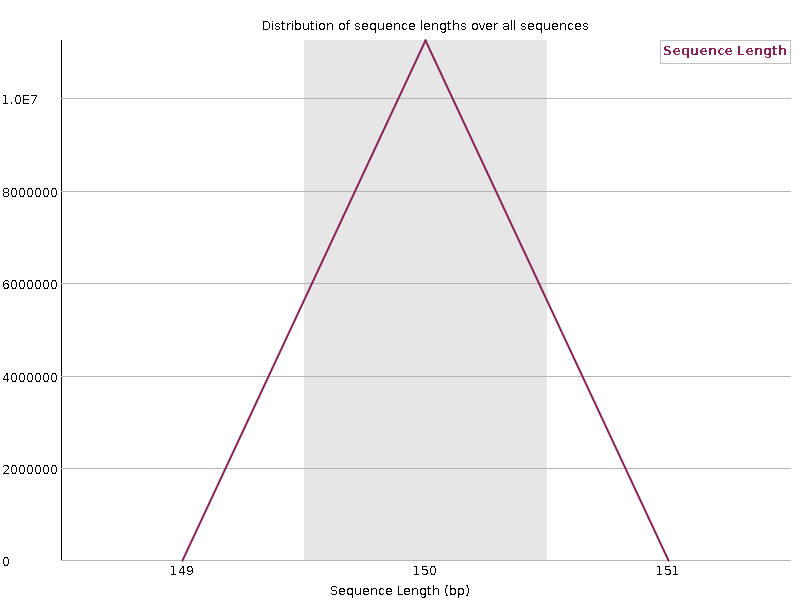
\includegraphics[width=0.7\textwidth,height=\textheight]{./assets/27_fqc_len_dist.png}

}

\caption{Sequence Length Distribution plot of SRR8306028.}

\end{figure}

\hypertarget{sequence-duplication-levels}{%
\subsection{Sequence Duplication
Levels}\label{sequence-duplication-levels}}

This module counts the degree of duplication for every sequence in a
library and creates a plot showing the relative number of sequences with
different degrees of duplication. A low level of duplication may
indicate a very high level of coverage of the target sequence, but a
high level of duplication is more likely to indicate some kind of
enrichment bias (eg PCR over amplification).

\begin{figure}

{\centering 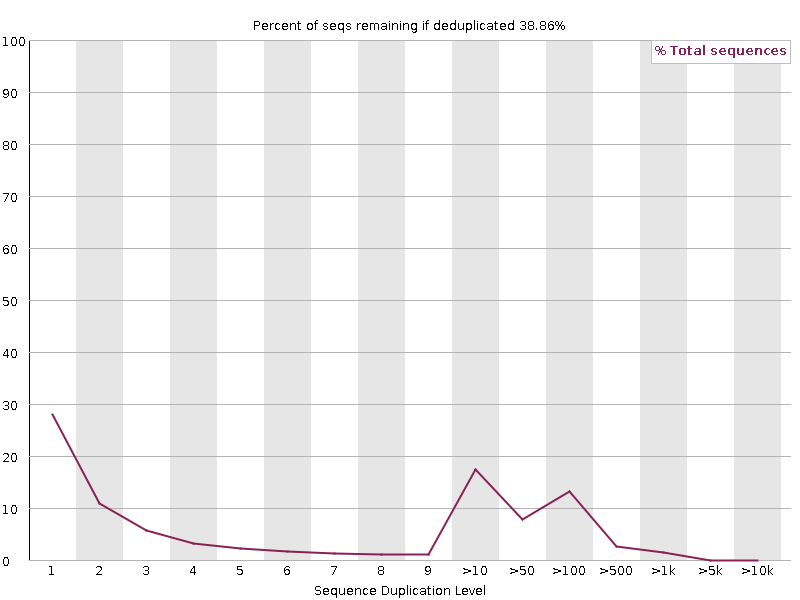
\includegraphics[width=0.7\textwidth,height=\textheight]{./assets/28_fqc_seq_dups.png}

}

\caption{Sequence Duplication Levels plot of SRR8306028.}

\end{figure}

\hypertarget{overrepresented-sequences}{%
\subsection{Overrepresented sequences}\label{overrepresented-sequences}}

This module lists all sequences that make up more than 0.1\% of the
first 100,000 sequences examined. For each overrepresented sequence, the
program searches for matches in a database of common impurities and
reports the best match found. However, finding a hit doesn't mean that
this is the source of the contamination, but may point you in the right
direction.

\hypertarget{adapter-content}{%
\subsection{Adapter Content}\label{adapter-content}}

This plot shows the cumulative percentage of adapter sequences used for
sequencing this library at each position. Most adapter sequences found
in Illumina RNA-Seq libraries are Illumina Universal Adapters. This
module issues a warning if a sequence is present in more than 5\% of all
reads. This module issues a warning if a sequence is present in more
than 10\% of all reads. If the adapter sequence is present in more than
1\% of the sequence library, adapter trimming is considered.

\begin{figure}

{\centering 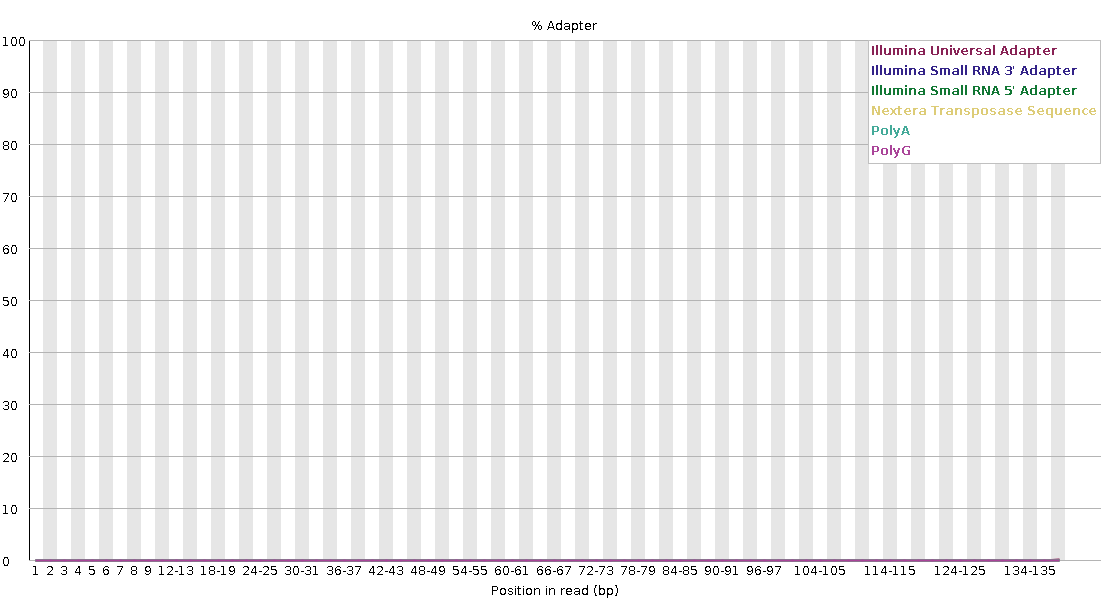
\includegraphics[width=0.7\textwidth,height=\textheight]{./assets/30_adapter_content.png}

}

\caption{Adapter Content of SRR8306028.}

\end{figure}

\begin{tcolorbox}[enhanced jigsaw, breakable, bottomrule=.15mm, left=2mm, coltitle=black, opacityback=0, colframe=quarto-callout-note-color-frame, toprule=.15mm, opacitybacktitle=0.6, colbacktitle=quarto-callout-note-color!10!white, bottomtitle=1mm, colback=white, toptitle=1mm, titlerule=0mm, rightrule=.15mm, arc=.35mm, title=\textcolor{quarto-callout-note-color}{\faInfo}\hspace{0.5em}{Activity}, leftrule=.75mm]

To further combine all the QC results into a single interactive HTML
file, we'd suggested to use \texttt{multiqc} software to combine it.

\begin{Shaded}
\begin{Highlighting}[]
\ExtensionTok{conda}\NormalTok{ activate qc}
\end{Highlighting}
\end{Shaded}

Then, run multiqc

\begin{Shaded}
\begin{Highlighting}[]
\ExtensionTok{multiqc} \AttributeTok{{-}{-}filename}\NormalTok{ QCreport\_before\_trim }\DataTypeTok{\textbackslash{}}
\NormalTok{{-}{-}outdir 02\_QC/ }\DataTypeTok{\textbackslash{}}
\NormalTok{{-}{-}dirs 02\_QC/fastQC\_before\_trim/}
\end{Highlighting}
\end{Shaded}

Output files:

\begin{verbatim}
- QCreport_before_trim_data
   ├── multiqc_citations.txt
   ├── multiqc_data.json
   ├── multiqc_fastqc.txt
   ├── multiqc_general_stats.txt
   ├── multiqc.log
   └── multiqc_sources.txt
- QCreport_before_trim.html
\end{verbatim}

\end{tcolorbox}

\hypertarget{adapter-trimming-with-cutadapt}{%
\section{Adapter Trimming with
Cutadapt}\label{adapter-trimming-with-cutadapt}}

Cutadapt is a tool to remove sequencing adapters, primers, poly-A tails
and other types of unwanted sequence from your high-throughput
sequencing reads. Cutadapt supports both FASTQ and FASTA file format for
trimming.

Several types of sequencing adapters have been used nowaday. We have to
know which adapter found in our sequencing library. Fortunately,
Illumina provide a manual of
\href{https://support.illumina.com/downloads/illumina-adapter-sequences-document-1000000002694.html}{Illumina
Adapter Sequences} that used in different types of sequencing. As
mentioned, most of RNA-Seq library sequenced by Illumina used Illumina
TruSeq Single Indexes, which is
\texttt{AGATCGGAAGAGCACACGTCTGAACTCCAGTCA} and
\texttt{AGATCGGAAGAGCGTCGTGTAGGGAAAGAGTGT} flanked at the 5' end of
forward reads and 3' end of reverse reads, respectively.

Fortunately, the dataset that will be used is free of apadter sequences
examined from the \protect\hyperlink{adapter-content}{adapter content}
from FastQC result. \textbf{\emph{So this command will just show as a
demo for your future project.}}

An example command of Cutadapt as follow.

\begin{Shaded}
\begin{Highlighting}[]
\ExtensionTok{cutadapt} \AttributeTok{{-}{-}cores}\NormalTok{ 2 }\DataTypeTok{\textbackslash{}}
\NormalTok{{-}u 10 }\AttributeTok{{-}U}\NormalTok{ 10 }\DataTypeTok{\textbackslash{}}
\NormalTok{{-}a AGATCGGAAGAGCACACGTCTGAACTCCAGTCA }\DataTypeTok{\textbackslash{}}
\NormalTok{{-}A AGATCGGAAGAGCGTCGTGTAGGGAAAGAGTGT }\DataTypeTok{\textbackslash{}}
\NormalTok{{-}o }\OperatorTok{\textless{}}\NormalTok{output\_forward.fastq}\OperatorTok{\textgreater{}} \DataTypeTok{\textbackslash{}}
\NormalTok{{-}p }\OperatorTok{\textless{}}\NormalTok{output\_reverse.fastq}\OperatorTok{\textgreater{}} \DataTypeTok{\textbackslash{}}
\OperatorTok{\textless{}}\NormalTok{input\_forward.fastq}\OperatorTok{\textgreater{}} \OperatorTok{\textless{}}\NormalTok{input\_reverse.fastq}\OperatorTok{\textgreater{}}
\end{Highlighting}
\end{Shaded}

According to the command, we specify number of CPU threads in
\texttt{-\/-cores}. We remove 10 bases directly from each end of read,
\texttt{-u} for forward and \texttt{-U} for reverse reads. Then we
specify the adapter sequences as mentioned above in \texttt{a} and
\texttt{A}. And the paths for forward and reverse reads output files in
\texttt{-o} and \texttt{-p}, respectively.

\hypertarget{reference-sources-1}{%
\section{Reference Sources}\label{reference-sources-1}}

\begin{itemize}
\item
  \href{https://hbctraining.github.io/Intro-to-rnaseq-hpc-O2/lessons/02_assessing_quality.html}{Quality
  Control of FASTQ files} from Harvard Chan Bioinformatics Core (HBC)
  training (Accessed on 1 Mar 2023).
\item
  \href{https://www.bioinformatics.babraham.ac.uk/projects/fastqc/}{FastQC
  official website} from Babraham Bioinformatics (Accessed on 1 Mar
  2023).
\item
  \href{https://www.bioinformatics.babraham.ac.uk/projects/fastqc/Help/}{FastQC
  Documentation} from Babraham Bioinformatics (Accessed on 1 Mar 2023).
\item
  \href{https://cutadapt.readthedocs.io/en/stable/guide.html}{Cutadapt
  4.2 Documentation} (Accessed on 1 Mar 2023).
\item
  \href{https://support.illumina.com/downloads/illumina-adapter-sequences-document-1000000002694.html}{Illumina
  Adapter Sequences} (Accessed on 1 Mar 2023).
\end{itemize}

\bookmarksetup{startatroot}

\hypertarget{de-novo-assembly-with-trinity}{%
\chapter{De novo Assembly with
Trinity}\label{de-novo-assembly-with-trinity}}

Trinity is a promosing tool for de novo full-length transcriptome
assembly that continually developed since 2011. Trinity assembles reads
by constructs many individual de Bruijn graphs, each representing the
transcriptional complexity at a given gene or locus, that originated
from the different nucleotide in the same position, and then processes
each graph independently to extract full-length splicing isoforms and to
tease apart transcripts derived from paralogous genes (Grabherr et al.
2011; Haas et al. 2013). Each assembled contig is will refer to a
transcript.

\begin{figure}

{\centering 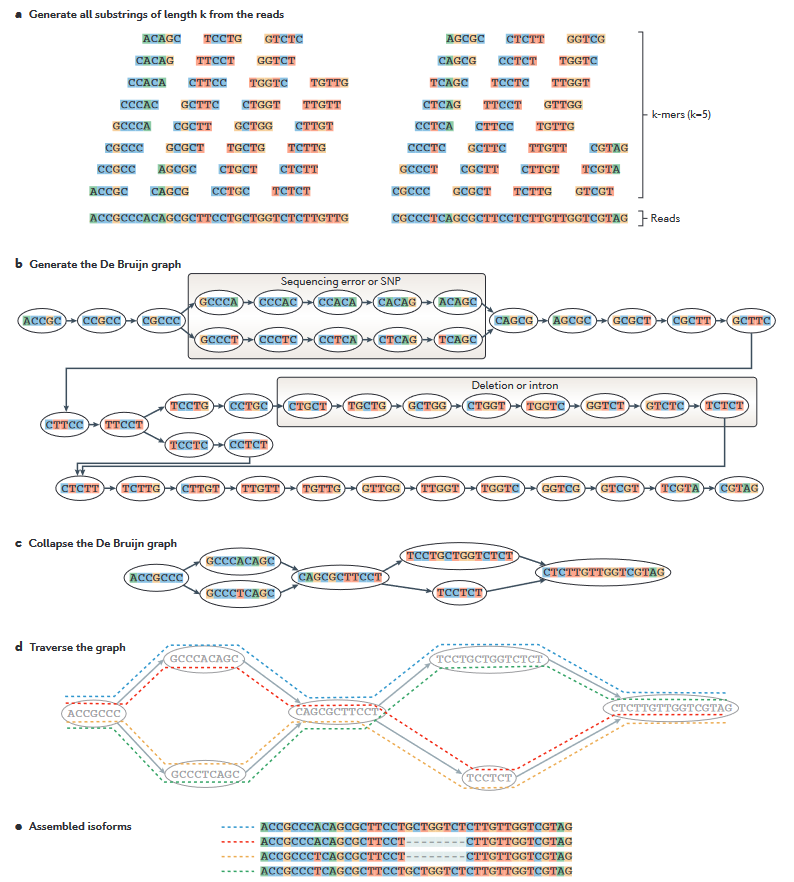
\includegraphics{assets/38_denovo_assembly_concept.png}

}

\caption{Overview of the concept of de novo transcriptome assembly.
Clean reads are divided into k-mers, i.e., in this figure k = 5, which
means that a read is divided into many fragments, each fragment
containing 5 bases. Then, de Bruijn graphs are stitched from a pool of
billions of k-mers (b). During sequencing, read fragments originating
from the same spot or derived from the same gene may even have a
nucleotide change at the same position, which may be either true
polymorphisms or sequencing errors, so that similar k-mer sequences are
joined together and routing to adjacent k-mers (c). The bulges in the
graphs represent variations within the graph complex. Each graph complex
represents a gene that can split into many transcript isoforms during
traversion (d) to eventually obtain the assembled transcript library
(e). For more details, please see Martin and Wang (2011).}

\end{figure}

Trinity can construct genomes without genome information and enables
transcript construction in non-model organisms where genome assembly is
not yet available, or that do not achieve successful chromosome-level or
full assembly. Downstream processes, such as transcript assembly
completeness analysis, transcript abundance estimation, and
identification of differentially expressed genes, can also be performed
with Trinity and its built-in utilities commands.

For de novo assembly in fast and efficient way for limited computational
resources available, we prepared the downsized reads that derived from
the SRA accessions that we already retrieved from NCBI SRA database from
the previous chapter.

During de novo assembly, the longest and the heaviest computation
resource required for constructing and stitching billions of de Bruijn
graphs. Very deep sequencing libraries may failed of these processes.
Therefore, normalizing or downsizing sequence reads before de novo
assembly is efficient way to proceed it. In brief, we downsized sequence
reads using built-in Trinity command
\texttt{insilico\_read\_normalization.pl} as follow. \emph{This just
inform all participant to the source of raw data that they will perform
assembly.}

\begin{Shaded}
\begin{Highlighting}[]
\ExtensionTok{insilico\_read\_normalization.pl} \DataTypeTok{\textbackslash{}}
\NormalTok{{-}{-}seqType fq }\DataTypeTok{\textbackslash{}}
\NormalTok{{-}{-}JM 100G }\DataTypeTok{\textbackslash{}}
\NormalTok{{-}{-}max\_cov 10 }\DataTypeTok{\textbackslash{}}
\NormalTok{{-}{-}left 01\_Rawdata/}\PreprocessorTok{*}\NormalTok{\_1.fastq }\DataTypeTok{\textbackslash{}}
\NormalTok{{-}{-}right 01\_Rawdata/}\PreprocessorTok{*}\NormalTok{\_2.fastq }\DataTypeTok{\textbackslash{}}
\NormalTok{{-}{-}pairs\_together }\DataTypeTok{\textbackslash{}}
\NormalTok{{-}{-}CPU 50 }\DataTypeTok{\textbackslash{}}
\NormalTok{{-}{-}output 03\_assembly}
\end{Highlighting}
\end{Shaded}

Trinity \texttt{insilico\_read\_normalization.pl} uses forward and
reverse reads input from \texttt{-\/-left} and \texttt{–-right}
parameters by reduce the maximum coverage depth (\texttt{-\/-max\_cov})
observed to 10x, and retain only paired reads in
\texttt{-\/-pairs\_together}.

The output file given as follow:

\begin{verbatim}
<ls 03_assembly>
\end{verbatim}

\hypertarget{running-trinity}{%
\section{Running Trinity}\label{running-trinity}}

Trinity is run via the script \texttt{Trinity}:

\begin{Shaded}
\begin{Highlighting}[]
\ExtensionTok{Trinity} \AttributeTok{{-}{-}seqType}\NormalTok{ fq }\DataTypeTok{\textbackslash{}}
\NormalTok{{-}{-}max\_memory 6G }\DataTypeTok{\textbackslash{}}
\NormalTok{{-}{-}CPU 2 }\DataTypeTok{\textbackslash{}}
\NormalTok{{-}{-}left 01\_rawdata/left.fq }\DataTypeTok{\textbackslash{}}
\NormalTok{{-}{-}right 01\_rawdata/right.fq }\DataTypeTok{\textbackslash{}}
\NormalTok{{-}{-}no\_normalize\_reads}
\end{Highlighting}
\end{Shaded}

By this command, Trinity take the input forward and reverse reads from
\texttt{-\/-left} and \texttt{–-right}, respectively. By default, de
novo assembly with Trinity will perform in silico read normalization by
itself. Since we have already normalized the sequence reads file prior
to assembly, this step will skip the normalization step by add
\texttt{-\/-no\_normalize\_reads} to the command. All other arguments
will use with the default parameters.

The given results in \texttt{03\_assembly} directory are:

xxxxxxxx.

\hypertarget{transcript-assembly-quality-assessment}{%
\section{Transcript Assembly Quality
Assessment}\label{transcript-assembly-quality-assessment}}

\bookmarksetup{startatroot}

\hypertarget{estimating-abundance-and-differential-expression-analysis-of-genes}{%
\chapter{Estimating Abundance and Differential Expression Analysis of
Genes}\label{estimating-abundance-and-differential-expression-analysis-of-genes}}

Differential gene expression analysis is a statistical method that uses
count data to determine significant changes between experimental groups.
For example, transcriptional changes of stress-induced genes in plant
leaves under water deficit compared to normal conditions are examined.
Count data can be transcript, gene, exon, and noncoding characteristics.

To perform differential gene expression analysis with the Trinity
integrated extensions, you will need the assembled transcripts/genes
from the previous step and clean reads (and their replicates) from your
experiment to assign to the assembled transcripts/genes and count the
number of reads assigned to those transcripts/genes.

\hypertarget{estimating-transcript-abundance}{%
\section{Estimating Transcript
Abundance}\label{estimating-transcript-abundance}}

This part will adopted from Trinity's Wiki
\href{https://github.com/trinityrnaseq/trinityrnaseq/wiki/Trinity-Transcript-Quantification}{Trinity
Transcript Quantification}.

There are two different methods for quantifying reads mapped to the
reference, by using the alignment-based (RSEM) and alignment-free
(salmon, kallisto) qualtifiers. In this workshop, we'll use the salmon,
an ultra-fast alignment and quantification tool, to count number of
reads mapped to the assembled gene.

\begin{tcolorbox}[enhanced jigsaw, breakable, bottomrule=.15mm, left=2mm, coltitle=black, opacityback=0, colframe=quarto-callout-tip-color-frame, toprule=.15mm, opacitybacktitle=0.6, colbacktitle=quarto-callout-tip-color!10!white, bottomtitle=1mm, colback=white, toptitle=1mm, titlerule=0mm, rightrule=.15mm, arc=.35mm, title=\textcolor{quarto-callout-tip-color}{\faLightbulb}\hspace{0.5em}{Tip}, leftrule=.75mm]

You can see the usage of the command you wsh to perform by type the
command followed by \texttt{-\/-help}, or \texttt{-h}. For example, to
see the usage of

\begin{verbatim}
align_and_estimate_abundance.pl -h
\end{verbatim}

\end{tcolorbox}

\begin{tcolorbox}[enhanced jigsaw, breakable, bottomrule=.15mm, left=2mm, coltitle=black, opacityback=0, colframe=quarto-callout-note-color-frame, toprule=.15mm, opacitybacktitle=0.6, colbacktitle=quarto-callout-note-color!10!white, bottomtitle=1mm, colback=white, toptitle=1mm, titlerule=0mm, rightrule=.15mm, arc=.35mm, title=\textcolor{quarto-callout-note-color}{\faInfo}\hspace{0.5em}{Activity}, leftrule=.75mm]

Now we will align and count reads mapped to the reference assembled
transcripts using buit-in utility
\texttt{align\_and\_estimate\_abundance.pl} using the following
commands.

\begin{enumerate}
\def\labelenumi{\arabic{enumi}.}
\item
  Go to working directory

\begin{Shaded}
\begin{Highlighting}[]
\BuiltInTok{cd}\NormalTok{ \textasciitilde{}/Cpa\_RNASeq}
\end{Highlighting}
\end{Shaded}

  The working directory should contain the following subdirectories.
\end{enumerate}

\begin{verbatim}
        Cpa_RNASeq
        ├── 01_Rawdata
        ├── 02_QC
        ├── 03_assembly
        ├── 04_DE_analysis
        └── 05_annotation
\end{verbatim}

\begin{enumerate}
\def\labelenumi{\arabic{enumi}.}
\setcounter{enumi}{1}
\item
  Estimating Transcript Abundance

\begin{Shaded}
\begin{Highlighting}[]
\ExtensionTok{align\_and\_estimate\_abundance.pl} \DataTypeTok{\textbackslash{}}
\NormalTok{{-}{-}transcripts 03\_assembly/trinity\_out\_dir.Trinity.fasta }\DataTypeTok{\textbackslash{}}
\NormalTok{{-}{-}seqType fq }\DataTypeTok{\textbackslash{}}
\NormalTok{{-}{-}samples\_file sample\_list.tsv }\DataTypeTok{\textbackslash{}}
\NormalTok{{-}{-}est\_method salmon }\DataTypeTok{\textbackslash{}}
\NormalTok{{-}{-}gene\_trans\_map 03\_assembly/trinity\_out\_dir.Trinity.fasta.gene\_trans\_map }\DataTypeTok{\textbackslash{}}
\NormalTok{{-}{-}thread\_count 2 }\DataTypeTok{\textbackslash{}}
\NormalTok{{-}{-}prep\_reference}
\end{Highlighting}
\end{Shaded}
\end{enumerate}

\end{tcolorbox}

Parameter descriptions of \texttt{align\_and\_estimate\_abundance.pl}:
the assembled transcripts flagged in \texttt{-\/-transcripts},
\texttt{-\/-seqType} indicates file format of reads that will be mappped
to the reference transcripts.

A list of read files will be contained in the metadata file
sample\_list.tsv in the parameter \texttt{-\/-samples\_file}, which we
have prepared for you. In short, the sample list will be prepared in a
tab-delimited text file indicating the relationships between biological
replicates. For example,

\begin{verbatim}
dark    dark_1  01_Rawdata/SRR8306034_1.fastq   01_Rawdata/SRR8306034_2.fastq
dark    dark_2  01_Rawdata/SRR8306029_1.fastq   01_Rawdata/SRR8306029_2.fastq
dark    dark_3  01_Rawdata/SRR8306028_1.fastq   01_Rawdata/SRR8306028_2.fastq
normal_light    normal_light_1  01_Rawdata/SRR8306033_1.fastq   01_Rawdata/SRR8306033_2.fastq
normal_light    normal_light_2  01_Rawdata/SRR8306032_1.fastq   01_Rawdata/SRR8306032_2.fastq
normal_light    normal_light_3  01_Rawdata/SRR8306035_1.fastq   01_Rawdata/SRR8306035_2.fastq
\end{verbatim}

The first column indicates the study experimental groups, followed by
their biological replicates in the second column, and the forward and
reverse sequence read files belong to their biological replicate. It's
important that the file path begins with the directory in which you'll
be working so that the programs can correctly route to the files.

Next, define the read count estimation tool in \texttt{-\/-est\_method},
in this workshop we'll use salmon, and also estimate gene-level read
counts using information about gene-transcript relationships from the
\texttt{trinity\_out\_dir.Trinity.fasta.gene\_trans\_map} file that we
specified in the \texttt{-\/-gene\_trans\_map} parameter.

Output results are created in the current working directory separately
for experimental groups and biological replicates.

\begin{verbatim}
dark_1
    ├── aux_info/
    ├── cmd_info.json
    ├── lib_format_counts.json
    ├── libParams/
    ├── logs/
    ├── quant.sf
    └── quant.sf.genes
.
.
.
normal_light_3
    ├── aux_info/
    ├── cmd_info.json
    ├── lib_format_counts.json
    ├── libParams/
    ├── logs/
    ├── quant.sf
    └── quant.sf.genes
\end{verbatim}

\begin{tcolorbox}[enhanced jigsaw, breakable, bottomrule=.15mm, left=2mm, coltitle=black, opacityback=0, colframe=quarto-callout-note-color-frame, toprule=.15mm, opacitybacktitle=0.6, colbacktitle=quarto-callout-note-color!10!white, bottomtitle=1mm, colback=white, toptitle=1mm, titlerule=0mm, rightrule=.15mm, arc=.35mm, title=\textcolor{quarto-callout-note-color}{\faInfo}\hspace{0.5em}{Activity}, leftrule=.75mm]

According to the previous part, now we'll organize the directory to make
it tidy by moving all the results to the directory
\texttt{04\_\ DE\ \_analysis}.

\begin{verbatim}
``` bash
# make sure you're in ~/Cpa_RNASeq directory so that you can move the file correctly. 
mv dark* normal* 04_DE_analysis/
```

Then enter to the directory `04_DE_analysis`

``` bash
cd 04_DE_analysis
ls ./*
```
\end{verbatim}

\end{tcolorbox}

Expected result:

\begin{verbatim}
(trinity) jiratchaya@pslab1:~/Cpa_RNASeq/04_DE_analysis$ ls ./*
./dark_1:
aux_info  cmd_info.json  lib_format_counts.json  libParams  logs  quant.sf  quant.sf.genes

./dark_2:
aux_info  cmd_info.json  lib_format_counts.json  libParams  logs  quant.sf  quant.sf.genes

./dark_3:
aux_info  cmd_info.json  lib_format_counts.json  libParams  logs  quant.sf  quant.sf.genes

./normal_light_1:
aux_info  cmd_info.json  lib_format_counts.json  libParams  logs  quant.sf  quant.sf.genes

./normal_light_2:
aux_info  cmd_info.json  lib_format_counts.json  libParams  logs  quant.sf  quant.sf.genes

./normal_light_3:
aux_info  cmd_info.json  lib_format_counts.json  libParams  logs  quant.sf  quant.sf.genes
\end{verbatim}

after running salmon you'll find output files:

\begin{itemize}
\item
  \texttt{quant.sf} : transcript abundance estimates (generated by
  salmon)
\item
  \texttt{quant.sf.genes} : gene-level abundance estimates (generated
  here by summing transcript values)
\end{itemize}

Here's an example of \texttt{quant.sf.genes} file:

\begin{table}
\centering\begingroup\fontsize{11}{13}\selectfont

\begin{tabular}{l|r|r|r|r}
\hline
Name & Length & EffectiveLength & TPM & NumReads\\
\hline
TRINITY\_DN35101\_c0\_g1 & 248 & 35.30 & 0.00 & 0.00\\
\hline
TRINITY\_DN42970\_c0\_g1 & 215 & 24.82 & 7.15 & 3.00\\
\hline
TRINITY\_DN41199\_c0\_g1 & 280 & 47.38 & 0.00 & 0.00\\
\hline
TRINITY\_DN35784\_c0\_g1 & 247 & 34.96 & 6.77 & 4.00\\
\hline
TRINITY\_DN32682\_c0\_g1 & 275 & 45.30 & 0.00 & 0.00\\
\hline
TRINITY\_DN8538\_c0\_g1 & 1019 & 710.33 & 0.17 & 2.00\\
\hline
TRINITY\_DN2880\_c0\_g1 & 2376 & 2067.33 & 0.74 & 26.00\\
\hline
TRINITY\_DN9226\_c0\_g1 & 275 & 45.30 & 7.84 & 6.00\\
\hline
TRINITY\_DN3645\_c1\_g1 & 1175 & 866.33 & 0.40 & 5.82\\
\hline
TRINITY\_DN5921\_c0\_g2 & 368 & 94.72 & 4.37 & 7.00\\
\hline
\end{tabular}
\endgroup{}
\end{table}

\hypertarget{building-transcript-and-gene-expression-matrices}{%
\section{Building Transcript and Gene Expression
Matrices}\label{building-transcript-and-gene-expression-matrices}}

We use gene-level abundance matrices with the filename
\texttt{quant.sf.genes}, which are available in all results directories.
In this step, the utility \texttt{abundance\_estimates\_to\_matrix.pl}
is used to combine all separate count matrices from the file
\texttt{quant.sf.genes} in all result directories into a single matrix
file. By using salmon as \texttt{-\/-est\_method} and specifying the
parameter \texttt{-\/-gene\_trans\_map}, a gene abundance matrix is
created.

\begin{tcolorbox}[enhanced jigsaw, breakable, bottomrule=.15mm, left=2mm, coltitle=black, opacityback=0, colframe=quarto-callout-note-color-frame, toprule=.15mm, opacitybacktitle=0.6, colbacktitle=quarto-callout-note-color!10!white, bottomtitle=1mm, colback=white, toptitle=1mm, titlerule=0mm, rightrule=.15mm, arc=.35mm, title=\textcolor{quarto-callout-note-color}{\faInfo}\hspace{0.5em}{Activity}, leftrule=.75mm]

\begin{enumerate}
\def\labelenumi{\arabic{enumi}.}
\item
  Create abundance matrix

\begin{Shaded}
\begin{Highlighting}[]
\ExtensionTok{abundance\_estimates\_to\_matrix.pl} \AttributeTok{{-}{-}est\_method}\NormalTok{ salmon }\DataTypeTok{\textbackslash{}}
\NormalTok{{-}{-}gene\_trans\_map ../03\_assembly/trinity\_out\_dir.Trinity.fasta.gene\_trans\_map }\DataTypeTok{\textbackslash{}}
\NormalTok{{-}{-}name\_sample\_by\_basedir }\DataTypeTok{\textbackslash{}}
\PreprocessorTok{*}\NormalTok{/quant.sf.genes}
\end{Highlighting}
\end{Shaded}

  Expected result:

\begin{verbatim}
(trinity) jiratchaya@pslab1:~/Cpa_RNASeq/04_DE_analysis$ ls -l
total 4945
drwxrwx--- 1 root PSLab    4096 Mar  5 16:16 dark_1
drwxrwx--- 1 root PSLab    4096 Mar  5 16:16 dark_2
drwxrwx--- 1 root PSLab    4096 Mar  5 16:16 dark_3
drwxrwx--- 1 root PSLab    4096 Mar  5 16:16 normal_light_1
drwxrwx--- 1 root PSLab    4096 Mar  5 16:16 normal_light_2
drwxrwx--- 1 root PSLab    4096 Mar  5 16:16 normal_light_3
-rw-rw---- 1 root PSLab      67 Mar  6 13:29 salmon.gene.counts.matrix
-rw-rw---- 1 root PSLab      67 Mar  6 13:29 salmon.gene.TPM.not_cross_norm
-rw-rw---- 1 root PSLab 2736773 Mar  6 13:29 salmon.isoform.counts.matrix
-rw-rw---- 1 root PSLab 2297101 Mar  6 13:29 salmon.isoform.TPM.not_cross_norm
\end{verbatim}

  This command will generate 4 result files:

  \begin{itemize}
  \tightlist
  \item
    \texttt{salmon.gene.counts.matrix} is the estimated raw RNA-Seq
    counts in GENE level in all experimental groups.
  \item
    \texttt{salmon.gene.TPM.not\_cross\_norm} is the Transcript per
    Million (TPM) of RNA-Seq counts in GENE level in all experimental
    groups.
  \item
    \texttt{salmon.isoform.counts.matrix} is the estimated raw RNA-Seq
    counts in TRANSCRIPTS level in all experimental groups.
  \item
    \texttt{salmon.isoform.TPM.not\_cross\_norm} is the Transcript per
    Million (TPM) of RNA-Seq counts in TRANSCRIPTS level in all
    experimental groups.
  \end{itemize}
\end{enumerate}

\end{tcolorbox}

\hypertarget{quality-control-of-sample-read-counts-and-biological-replicates}{%
\section{Quality Control of Sample Read Counts and Biological
Replicates}\label{quality-control-of-sample-read-counts-and-biological-replicates}}

Once you've performed quantification for each experimental group, it's
good to examine the data to ensure that your biological replicates are
well correlated, and also to investigate relationships among your
samples.

It is critical that you identify any obvious differences between the
relationships between your sample and replicates, such as those
resulting from accidental mislabeling of sample replicates, strong
outliers, or batch effects, prior to further data analysis.

The Trinity's utility called \texttt{PtR} (pronounced as `Peter', stands
for Perl to R) can generate some exploratory data analysis that rely on
count matrix, such as compare difference between replicate, compare
difference between experimental groups, principal component analysis,
and so on.

\begin{tcolorbox}[enhanced jigsaw, breakable, bottomrule=.15mm, left=2mm, coltitle=black, opacityback=0, colframe=quarto-callout-note-color-frame, toprule=.15mm, opacitybacktitle=0.6, colbacktitle=quarto-callout-note-color!10!white, bottomtitle=1mm, colback=white, toptitle=1mm, titlerule=0mm, rightrule=.15mm, arc=.35mm, title=\textcolor{quarto-callout-note-color}{\faInfo}\hspace{0.5em}{Activity}, leftrule=.75mm]

Recheck the current working directory

\begin{Shaded}
\begin{Highlighting}[]
\BuiltInTok{pwd}
\end{Highlighting}
\end{Shaded}

You're in \texttt{\textasciitilde{}/Cpa\_RNASeq/04\_DE\_analysis}

\begin{enumerate}
\def\labelenumi{\arabic{enumi}.}
\item
  Prepare sample metadata from differential expression (DE) analysis

  The sample metadata table for analysis DE is different from the table
  used to estimate abundance. We only need the first two columns from
  this file to create a metadata table for analysis from DE. Therefore,
  we can use the following Bash command to create and edit a new file.

\begin{Shaded}
\begin{Highlighting}[]
\CommentTok{\# Go to \textasciitilde{}/Cpa\_RNASeq directory by change to upper directory}
\BuiltInTok{cd}\NormalTok{ ..}
\end{Highlighting}
\end{Shaded}

  Extract first 2 columns of the metadata for estimating read count to
  to a new file in \texttt{04\_DE\_analysis}

\begin{Shaded}
\begin{Highlighting}[]
\FunctionTok{cut} \AttributeTok{{-}f}\NormalTok{ 1{-}2 sample\_list.tsv }\OperatorTok{\textgreater{}}\NormalTok{ 04\_DE\_analysis/samples.txt}
\end{Highlighting}
\end{Shaded}

  Then dive back into 04\_DE\_analysis directory

\begin{Shaded}
\begin{Highlighting}[]
\BuiltInTok{cd}\NormalTok{ 04\_DE\_analysis}
\end{Highlighting}
\end{Shaded}

  See expected result file

\begin{verbatim}
(trinity) jiratchaya@pslab1:~/Cpa_RNASeq/04_DE_analysis$ cat samples.txt
dark    dark_1
dark    dark_2
dark    dark_3
normal_light    normal_light_1
normal_light    normal_light_2
normal_light    normal_light_3
\end{verbatim}
\end{enumerate}

\end{tcolorbox}

\hypertarget{compare-replicates-for-each-of-your-samples}{%
\subsection{Compare replicates for each of your
samples}\label{compare-replicates-for-each-of-your-samples}}

This step will use PtR to reads the matrix of counts, performs a
counts-per-million (CPM) data transformation followed by a log2
transform, and then generates a multi-page pdf file
\texttt{named\ \$\{sample\}.rep\_compare.pdf} for each of your samples,
including several useful plots

\begin{tcolorbox}[enhanced jigsaw, breakable, bottomrule=.15mm, left=2mm, coltitle=black, opacityback=0, colframe=quarto-callout-note-color-frame, toprule=.15mm, opacitybacktitle=0.6, colbacktitle=quarto-callout-note-color!10!white, bottomtitle=1mm, colback=white, toptitle=1mm, titlerule=0mm, rightrule=.15mm, arc=.35mm, title=\textcolor{quarto-callout-note-color}{\faInfo}\hspace{0.5em}{Activity}, leftrule=.75mm]

\begin{verbatim}
Compare replicates for each of your samples

``` bash
PtR --matrix salmon.isoform.counts.matrix \
--samples samples.txt --log2 --CPM \
--min_rowSums 10 \
--compare_replicates
```
\end{verbatim}

\end{tcolorbox}

These files will append more to your current working directories:

\begin{verbatim}
-rw-rw---- 1 root PSLab    4695 Mar  6 14:37 salmon.isoform.counts.matrix.R
-rw-rw---- 1 root PSLab 1990182 Mar  6 14:37 dark.rep_compare.pdf
-rw-rw---- 1 root PSLab 1828692 Mar  6 14:37 normal_light.rep_compare.pdf
-rw-rw---- 1 root PSLab 3558147 Mar  6 14:37 salmon.isoform.counts.matrix.minRow10.CPM.log2.dat
\end{verbatim}

The last 3 files are newly generated by this step. There's two PDF files
separated by experimental groups, \texttt{dark.rep\_compare.pdf} and
\texttt{normal\_light.rep\_compare.pdf}, and raw data for plots in
\texttt{.dat} file.

\begin{figure}

{\centering 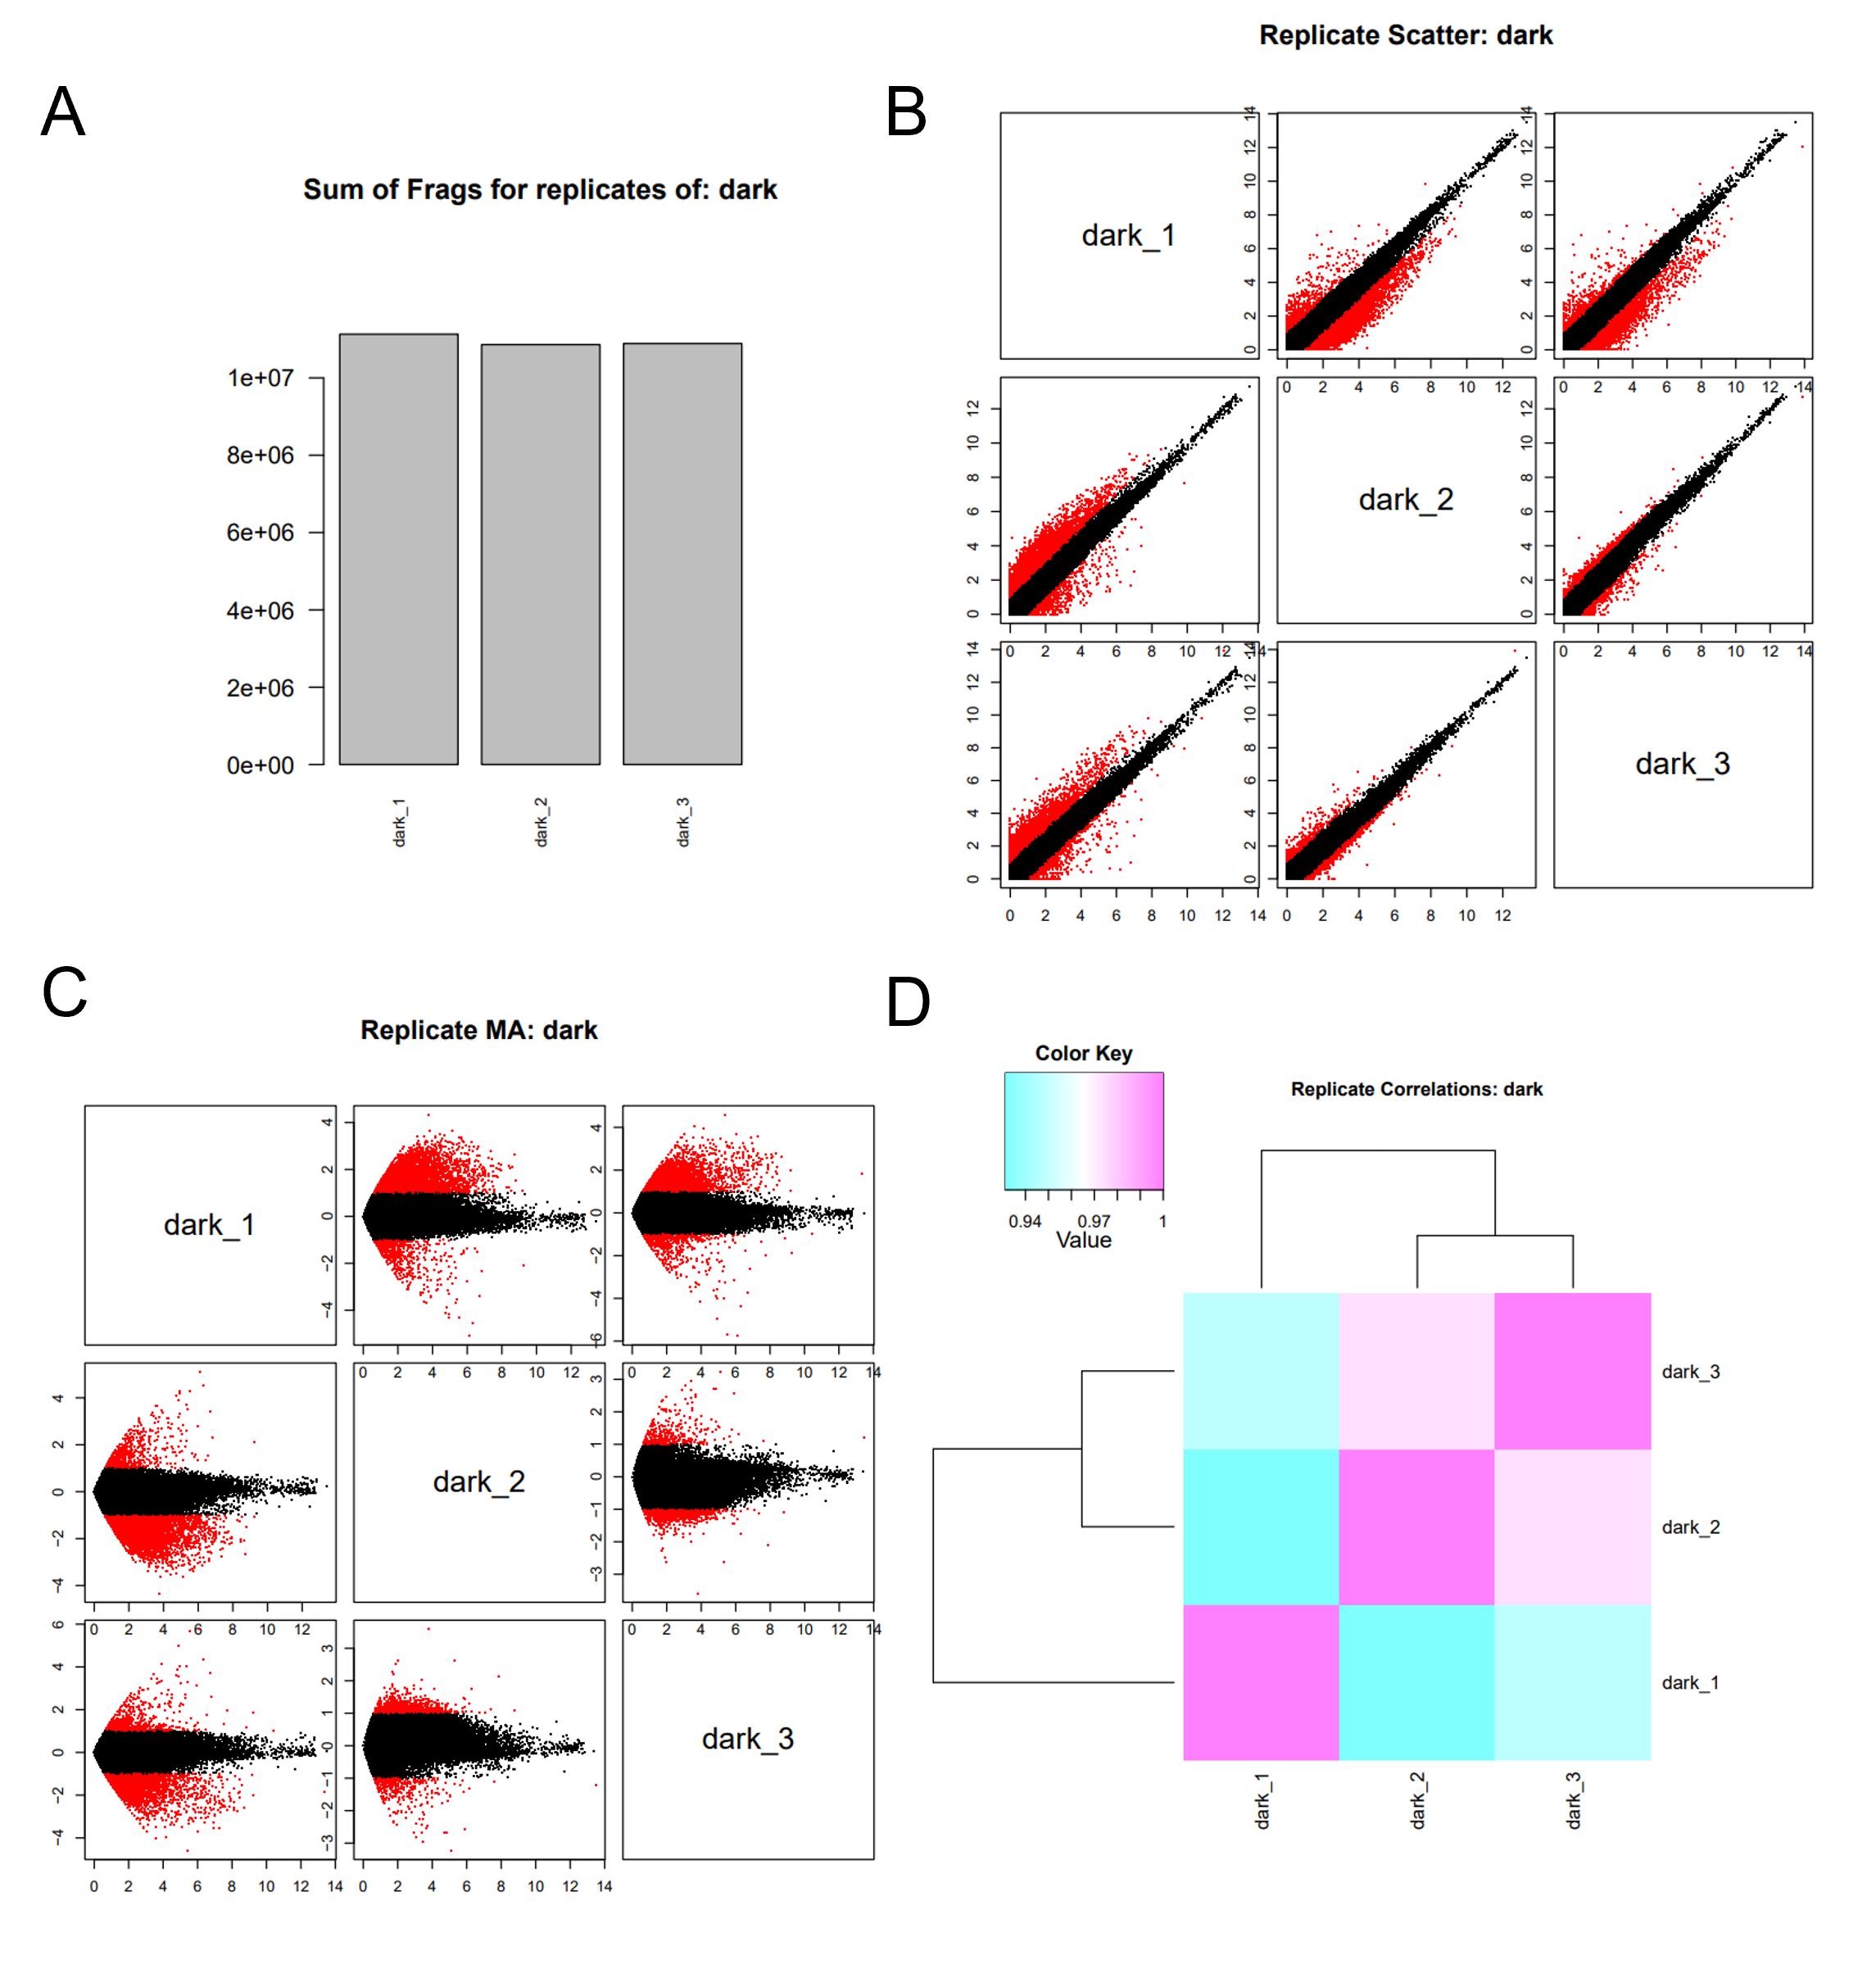
\includegraphics[width=0.7\textwidth,height=\textheight]{assets/32_trinity_compare_reps.png}

}

\caption{Example result of comparing biological replicates in Dark
samples. The figures were captured from \texttt{dark.rep\_compare.pdf}
file. (A) The sum of mapped fragments. (B) Pairwise comparisons of
replicate log(CPM) values, in which the data points more than 2-fold
different are highlighted in red. (C) The pairwise MA plots (x-axis:
mean log(CPM), y-axis log(fold\_change)). And, (D) A Replicate Pearson
correlation heatmap.}

\end{figure}

\hypertarget{compare-replicates-across-samples}{%
\subsection{Compare Replicates Across
Samples}\label{compare-replicates-across-samples}}

\begin{tcolorbox}[enhanced jigsaw, breakable, bottomrule=.15mm, left=2mm, coltitle=black, opacityback=0, colframe=quarto-callout-note-color-frame, toprule=.15mm, opacitybacktitle=0.6, colbacktitle=quarto-callout-note-color!10!white, bottomtitle=1mm, colback=white, toptitle=1mm, titlerule=0mm, rightrule=.15mm, arc=.35mm, title=\textcolor{quarto-callout-note-color}{\faInfo}\hspace{0.5em}{Activity}, leftrule=.75mm]

This command will generate a useful heatmap of pearson correlation
matrix of samples from two different experimental groups.

\begin{Shaded}
\begin{Highlighting}[]
    \ExtensionTok{PtR} \AttributeTok{{-}{-}matrix}\NormalTok{ salmon.isoform.counts.matrix }\DataTypeTok{\textbackslash{}}
    \AttributeTok{{-}{-}min\_rowSums}\NormalTok{ 10 }\DataTypeTok{\textbackslash{}}
    \AttributeTok{{-}{-}samples\_file}\NormalTok{ samples.txt }\DataTypeTok{\textbackslash{}}
    \AttributeTok{{-}{-}log2} \AttributeTok{{-}{-}CPM} \DataTypeTok{\textbackslash{}}
    \AttributeTok{{-}{-}sample\_cor\_matrix}
\end{Highlighting}
\end{Shaded}

\end{tcolorbox}

These files will append more to your current working directories:

\begin{verbatim}
-rw-rw---- 1 root PSLab    4012 Mar  6 15:02 salmon.isoform.counts.matrix.R
-rw-rw---- 1 root PSLab 3558147 Mar  6 15:02 salmon.isoform.counts.matrix.minRow10.CPM.log2.dat
-rw-rw---- 1 root PSLab     678 Mar  6 15:02 salmon.isoform.counts.matrix.minRow10.CPM.log2.sample_cor.dat
-rw-rw---- 1 root PSLab    6429 Mar  6 15:02 salmon.isoform.counts.matrix.minRow10.CPM.log2.sample_cor_matrix.pdf
\end{verbatim}

\begin{figure}

{\centering 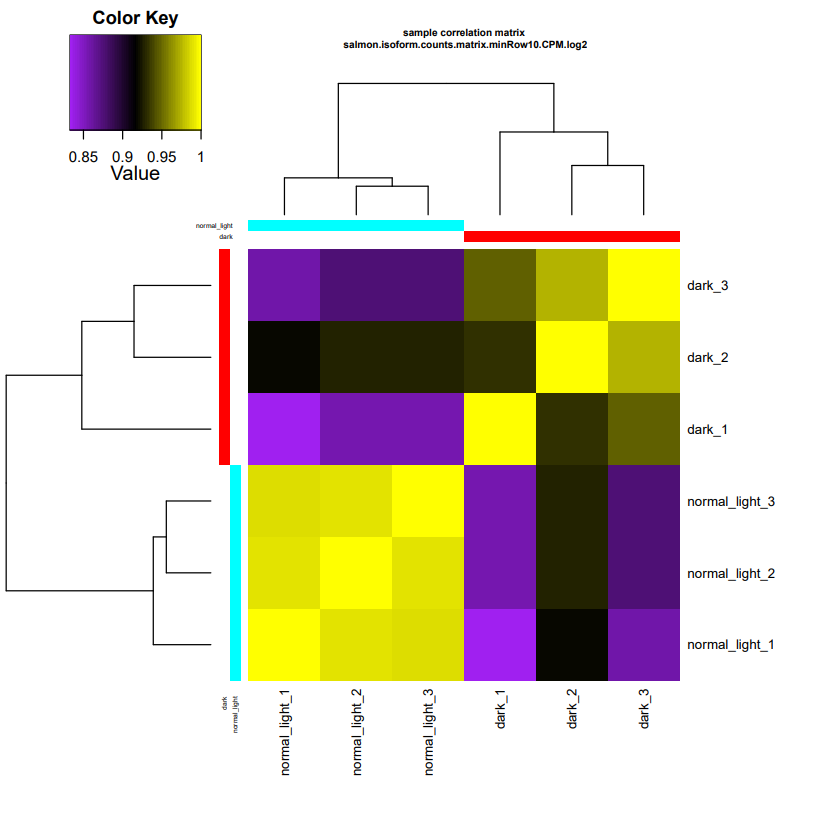
\includegraphics[width=0.7\textwidth,height=\textheight]{assets/33_sample_corr.png}

}

\caption{heatmap of pearson correlation coefficiant between Dark and
Normal light samples.}

\end{figure}

\hypertarget{principal-component-analysis-pca}{%
\subsection{Principal Component Analysis
(PCA)}\label{principal-component-analysis-pca}}

Another important analysis method to explore relationships among the
sample replicates is Principal Component Analysis (PCA).

You can find more explanation about PCA here: -
https://blog.bioturing.com/2018/06/14/principal-component-analysis-explained-simply/
- https://youtu.be/FgakZw6K1QQ

\begin{tcolorbox}[enhanced jigsaw, breakable, bottomrule=.15mm, left=2mm, coltitle=black, opacityback=0, colframe=quarto-callout-note-color-frame, toprule=.15mm, opacitybacktitle=0.6, colbacktitle=quarto-callout-note-color!10!white, bottomtitle=1mm, colback=white, toptitle=1mm, titlerule=0mm, rightrule=.15mm, arc=.35mm, title=\textcolor{quarto-callout-note-color}{\faInfo}\hspace{0.5em}{Activity}, leftrule=.75mm]

\begin{Shaded}
\begin{Highlighting}[]
    \ExtensionTok{PtR} \AttributeTok{{-}{-}matrix}\NormalTok{ salmon.isoform.counts.matrix }\DataTypeTok{\textbackslash{}}
    \AttributeTok{{-}{-}samples\_file}\NormalTok{ samples.txt }\DataTypeTok{\textbackslash{}}
    \AttributeTok{{-}{-}min\_rowSums}\NormalTok{ 10 }\AttributeTok{{-}{-}log2} \DataTypeTok{\textbackslash{}}
    \AttributeTok{{-}{-}CPM} \AttributeTok{{-}{-}center\_rows} \DataTypeTok{\textbackslash{}}
    \AttributeTok{{-}{-}prin\_comp}\NormalTok{ 3}
\end{Highlighting}
\end{Shaded}

\end{tcolorbox}

These files will append more to your current working directories:

\begin{verbatim}
-rw-rw---- 1 root PSLab    4789 Mar  6 15:18 salmon.isoform.counts.matrix.R
-rw-rw---- 1 root PSLab 4069112 Mar  6 15:18 salmon.isoform.counts.matrix.minRow10.CPM.log2.centered.dat
-rw-rw---- 1 root PSLab     756 Mar  6 15:18 salmon.isoform.counts.matrix.minRow10.CPM.log2.centered.PCA.prcomp.scores
-rw-rw---- 1 root PSLab 4163653 Mar  6 15:18 salmon.isoform.counts.matrix.minRow10.CPM.log2.centered.PCA.prcomp.loadings
-rw-rw---- 1 root PSLab    5446 Mar  6 15:18 salmon.isoform.counts.matrix.minRow10.CPM.log2.centered.prcomp.principal_components.pdf
\end{verbatim}

You can find the PCA plot in
\texttt{salmon.isoform.counts.matrix.minRow10.CPM.log2.centered.prcomp.principal\_components.pdf}.

\begin{figure}

{\centering 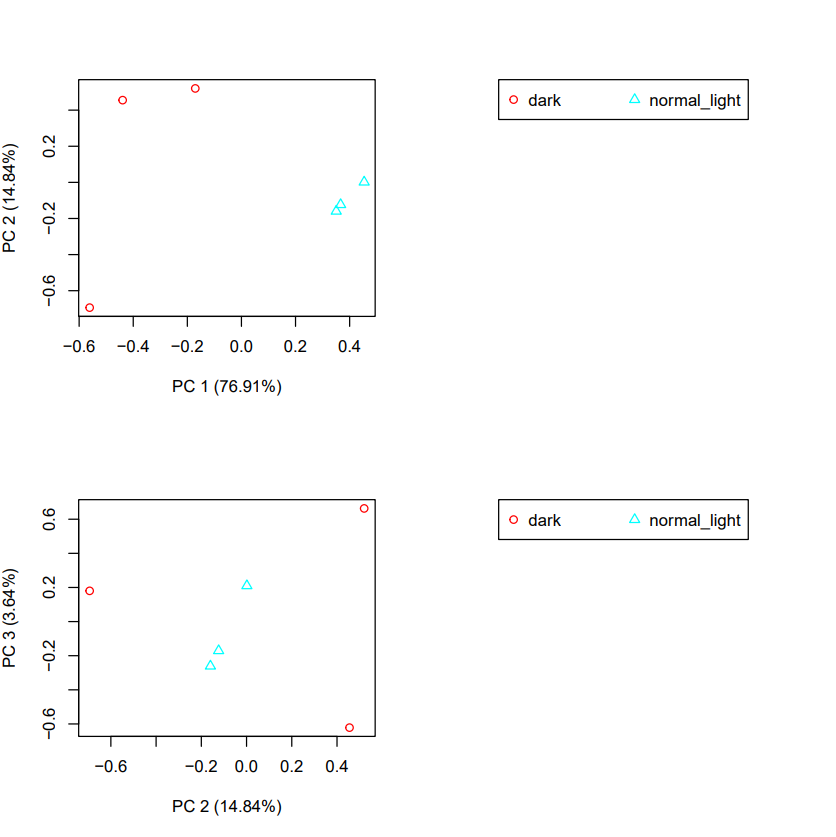
\includegraphics[width=0.7\textwidth,height=\textheight]{assets/34_PCA.png}

}

\caption{PCA plot.}

\end{figure}

We set the number of principal components (PC) to be calculated for only
first 3 PCs in \texttt{-\/-prin\_comp}. Which indicates that these PCs
will be plotted, as shown above, with PC1 vs.~PC2 and PC2 vs.~PC3. In
this example, the replicates cluster tightly according to sample type,
which is very reassuring.

\hypertarget{differential-expression-analysis}{%
\section{Differential Expression
Analysis}\label{differential-expression-analysis}}

Trinity also contains a built-in utility for DE analysis called
\texttt{run\_DE\_analysis.pl}, in which use the count matrix and sample
metadata file. Trinity provides support for several differential
expression analysis tools, currently including edgeR, DESeq2,
limma/voom, and ROTS.

DE analysis in Trinity will perform pairwise comparison of
gene/transcript expression. If the biological replicates are presented
for each sample, you should indicate this as we already created in our
metadata table \texttt{samples.txt}. Here we'll analyze DE genes in the
`transcript' level using the \texttt{salmon.isoform.counts.matrix} file.

\begin{tcolorbox}[enhanced jigsaw, breakable, bottomrule=.15mm, left=2mm, coltitle=black, opacityback=0, colframe=quarto-callout-note-color-frame, toprule=.15mm, opacitybacktitle=0.6, colbacktitle=quarto-callout-note-color!10!white, bottomtitle=1mm, colback=white, toptitle=1mm, titlerule=0mm, rightrule=.15mm, arc=.35mm, title=\textcolor{quarto-callout-note-color}{\faInfo}\hspace{0.5em}{Activity}, leftrule=.75mm]

DE analysis using DESeq2

\begin{Shaded}
\begin{Highlighting}[]
\ExtensionTok{run\_DE\_analysis.pl} \DataTypeTok{\textbackslash{}}
\NormalTok{{-}{-}matrix salmon.isoform.counts.matrix }\DataTypeTok{\textbackslash{}}
\NormalTok{{-}{-}method DESeq2 }\DataTypeTok{\textbackslash{}}
\NormalTok{{-}{-}samples\_file samples.txt }\DataTypeTok{\textbackslash{}}
\NormalTok{{-}{-}output DESeq2\_result}
\end{Highlighting}
\end{Shaded}

\end{tcolorbox}

After run the above command, the following directory will append to your
current working directory:

\begin{verbatim}
drwxrwx--- 1 root PSLab     688 Mar  6 15:42 DESeq2_result
\end{verbatim}

In this output directory, you'll find the following files for each of
the pairwise comparisons performed:

\begin{verbatim}
-rw-rw---- 1 root PSLab  972633 Mar  6 15:42 salmon.isoform.counts.matrix.dark_vs_normal_light.DESeq2.count_matrix
-rw-rw---- 1 root PSLab 4247784 Mar  6 15:42 salmon.isoform.counts.matrix.dark_vs_normal_light.DESeq2.DE_results
-rw-rw---- 1 root PSLab 2428272 Mar  6 15:42 salmon.isoform.counts.matrix.dark_vs_normal_light.DESeq2.DE_results.MA_n_Volcano.pdf
-rw-rw---- 1 root PSLab    1845 Mar  6 15:42 salmon.isoform.counts.matrix.dark_vs_normal_light.DESeq2.Rscript
\end{verbatim}

Result explanations:

\begin{itemize}
\item
  \texttt{salmon.isoform.counts.matrix.dark\_vs\_normal\_light.DESeq2.Rscript}
  is the R-script executed to perform the DE analysis.
\item
  \texttt{salmon.isoform.counts.matrix.dark\_vs\_normal\_light.DESeq2.count\_matrix}
  is an integer matrix of read count derived from the input file
  \texttt{salmon.isoform.counts.matrix}.
\item
  \texttt{salmon.isoform.counts.matrix.dark\_vs\_normal\_light.DESeq2.DE\_results}
  is the DE analysis results, including log fold change and statistical
  significance.
\item
  \texttt{salmon.isoform.counts.matrix.dark\_vs\_normal\_light.DESeq2.DE\_results.MA\_n\_Volcano.pdf}
  is MA and Volcano plots features found DE at the defined FDR will be
  colored red.
\end{itemize}

Here's an example of DE analysis result file
(\texttt{salmon.isoform.counts.matrix.dark\_vs\_normal\_light.DESeq2.DE\_results}):

\begin{table}
\centering\begingroup\fontsize{11}{13}\selectfont

\begin{tabular}{l|l|l|r|r|r|r|r|r|r|r}
\hline
  & sampleA & sampleB & baseMeanA & baseMeanB & baseMean & log2FoldChange & lfcSE & stat & pvalue & padj\\
\hline
TRINITY\_DN8082\_c0\_g1 & dark & normal\_light & 4685.731 & 17.948650 & 2351.8401 & 8.023585 & 0.3947937 & 20.32349 & 0 & 0\\
\hline
TRINITY\_DN281\_c0\_g1 & dark & normal\_light & 2406.185 & 9.827619 & 1208.0061 & 7.917578 & 0.3987747 & 19.85477 & 0 & 0\\
\hline
TRINITY\_DN902\_c0\_g1 & dark & normal\_light & 3515.942 & 5.151569 & 1760.5469 & 9.433323 & 0.4966128 & 18.99533 & 0 & 0\\
\hline
TRINITY\_DN801\_c0\_g2 & dark & normal\_light & 2100.468 & 4.052528 & 1052.2602 & 9.023139 & 0.4877916 & 18.49794 & 0 & 0\\
\hline
TRINITY\_DN38798\_c0\_g1 & dark & normal\_light & 1013.842 & 4.511975 & 509.1769 & 7.806389 & 0.4421257 & 17.65649 & 0 & 0\\
\hline
TRINITY\_DN10456\_c0\_g1 & dark & normal\_light & 3630.296 & 8.696336 & 1819.4963 & 8.698117 & 0.5004932 & 17.37909 & 0 & 0\\
\hline
TRINITY\_DN15271\_c1\_g1 & dark & normal\_light & 1503.228 & 6.205016 & 754.7166 & 7.908525 & 0.4612383 & 17.14629 & 0 & 0\\
\hline
TRINITY\_DN258\_c0\_g2 & dark & normal\_light & 2973.655 & 5.218821 & 1489.4370 & 9.144528 & 0.5358879 & 17.06425 & 0 & 0\\
\hline
TRINITY\_DN15130\_c0\_g1 & dark & normal\_light & 2019.010 & 4.727083 & 1011.8685 & 8.728308 & 0.5121991 & 17.04085 & 0 & 0\\
\hline
TRINITY\_DN1\_c0\_g2 & dark & normal\_light & 1107.861 & 6.860877 & 557.3612 & 7.312156 & 0.4304045 & 16.98903 & 0 & 0\\
\hline
\end{tabular}
\endgroup{}
\end{table}

An example of volcano plot for transcript-level differentially
expression analysis.

\begin{figure}

{\centering 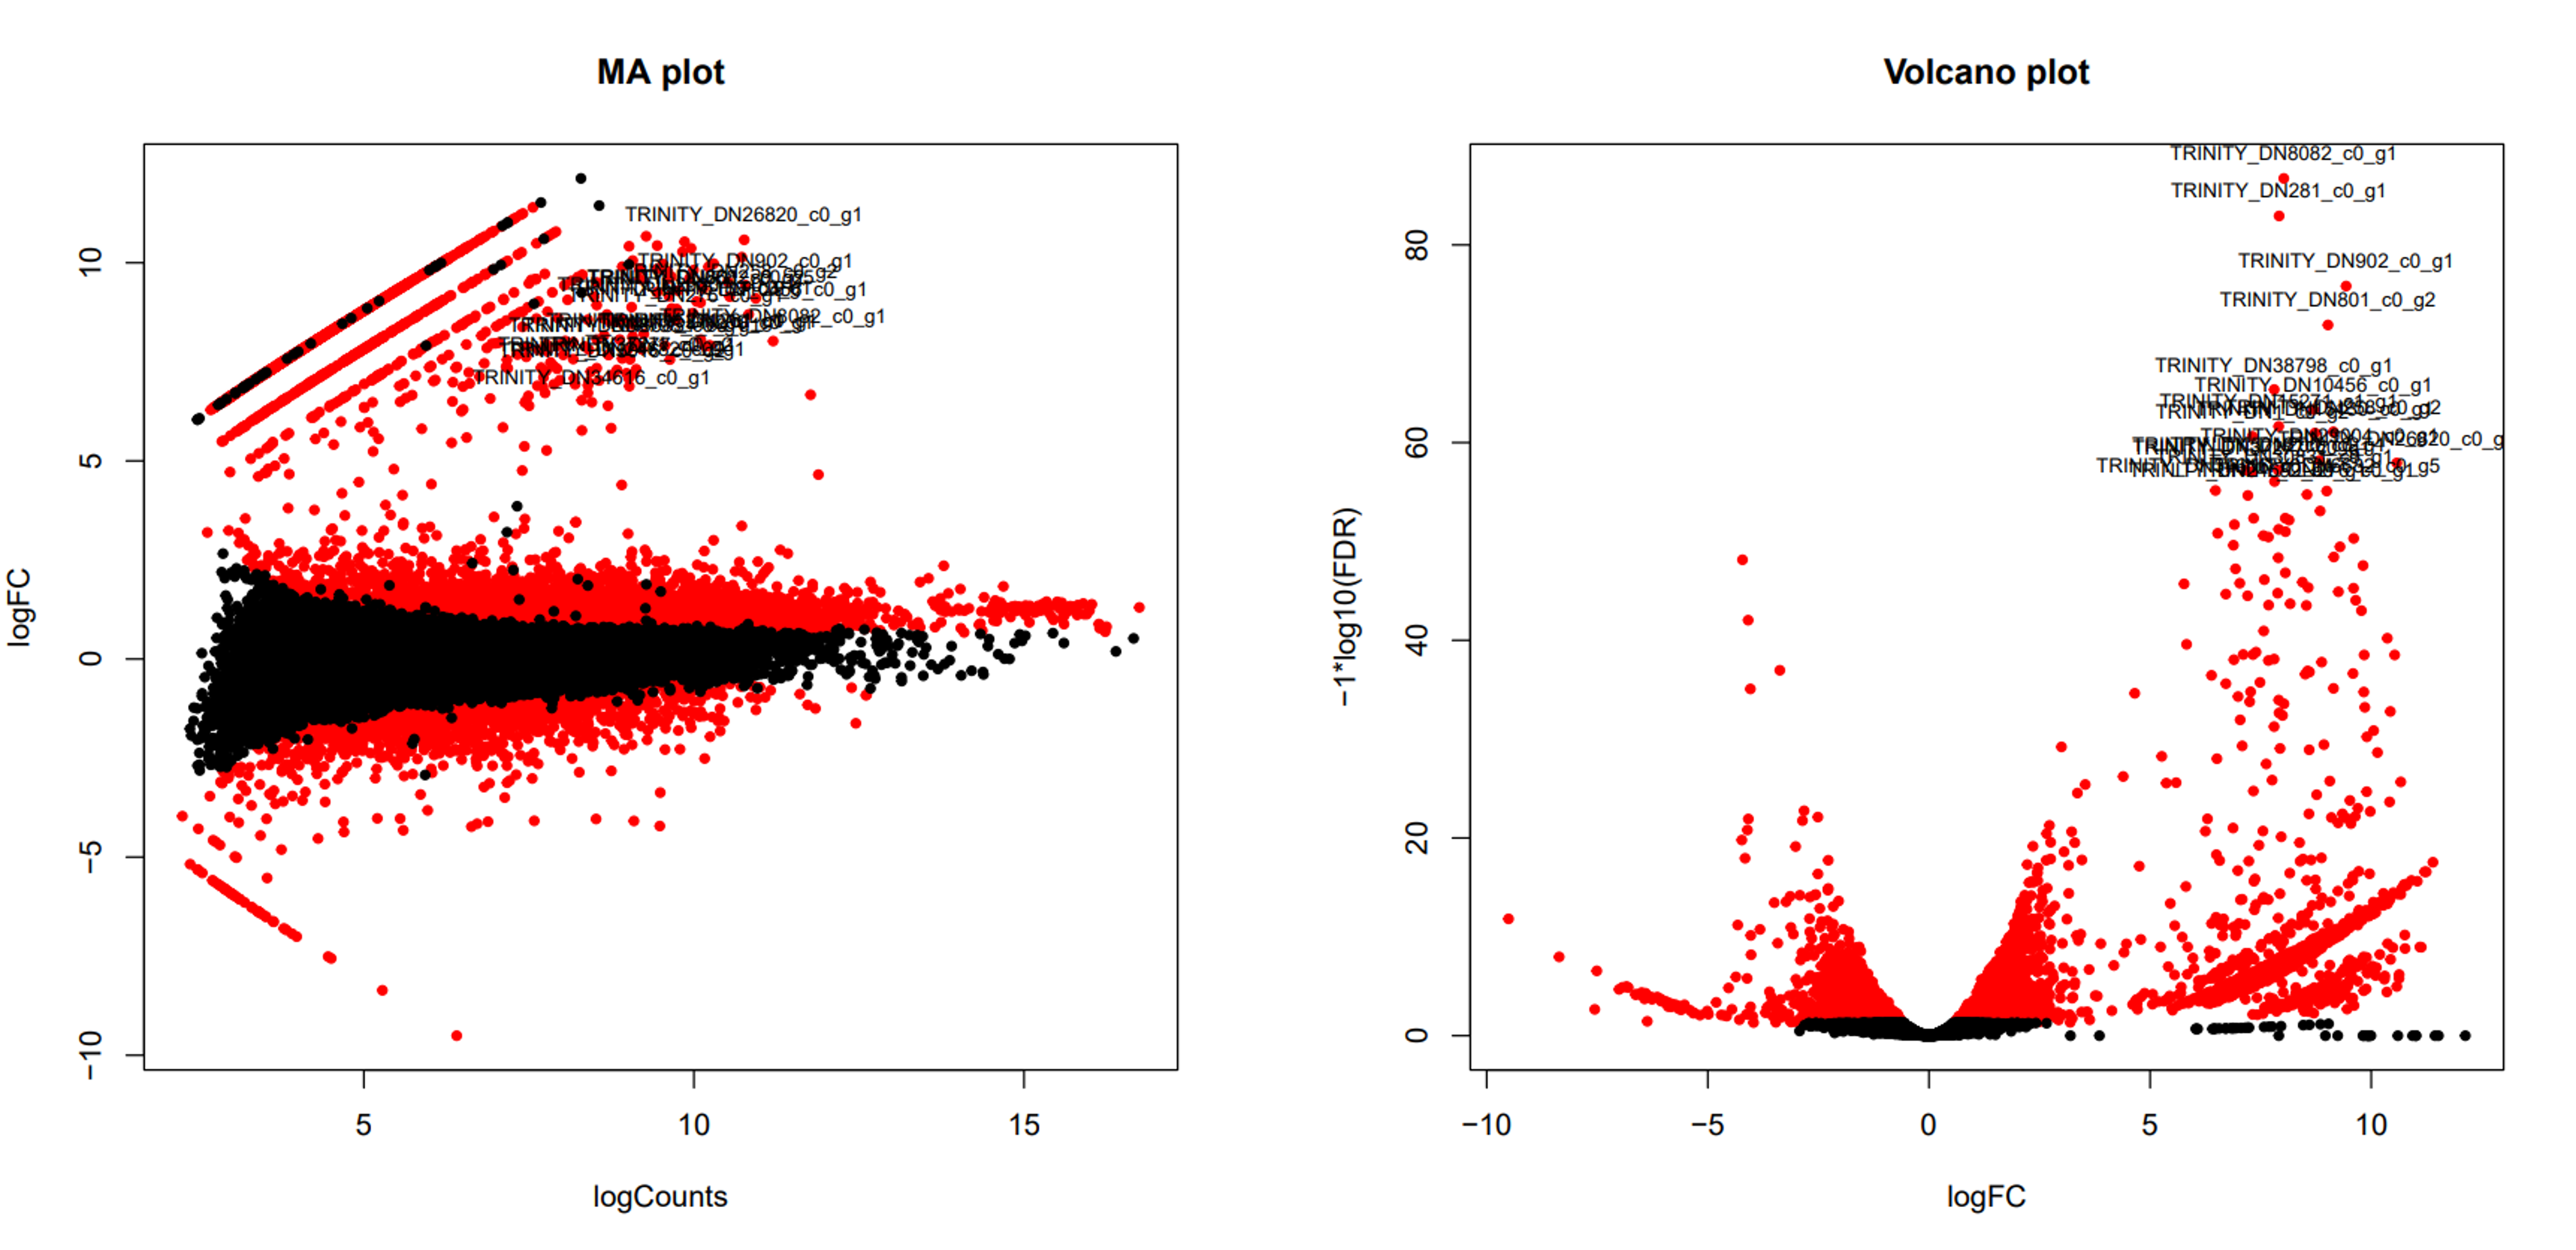
\includegraphics{assets/35_DE_plots.png}

}

\caption{(left) MA plot and (right) volcano plot.}

\end{figure}

\hypertarget{extracting-and-clustering-differentially-expressed-transcripts}{%
\section{Extracting and clustering differentially expressed
transcripts}\label{extracting-and-clustering-differentially-expressed-transcripts}}

An initial step in analyzing differential expression is to extract those
transcripts that are most differentially expressed (most significant FDR
and fold-changes) and to cluster the transcripts according to their
patterns of differential expression across the samples.

\begin{tcolorbox}[enhanced jigsaw, breakable, bottomrule=.15mm, left=2mm, coltitle=black, opacityback=0, colframe=quarto-callout-note-color-frame, toprule=.15mm, opacitybacktitle=0.6, colbacktitle=quarto-callout-note-color!10!white, bottomtitle=1mm, colback=white, toptitle=1mm, titlerule=0mm, rightrule=.15mm, arc=.35mm, title=\textcolor{quarto-callout-note-color}{\faInfo}\hspace{0.5em}{Activity}, leftrule=.75mm]

Extracting and clustering differentially expressed transcripts can run
using the following from within the DE output directory, by running the
following script:

\begin{Shaded}
\begin{Highlighting}[]
\BuiltInTok{cd}\NormalTok{ DESeq2\_result/}
\ExtensionTok{analyze\_diff\_expr.pl} \DataTypeTok{\textbackslash{}}
\NormalTok{{-}{-}matrix salmon.isoform.counts.matrix.dark\_vs\_normal\_light.DESeq2.count\_matrix }\DataTypeTok{\textbackslash{}}
\NormalTok{{-}P 0.001 }\DataTypeTok{\textbackslash{}}
\NormalTok{{-}C 2 }\DataTypeTok{\textbackslash{}}
\NormalTok{{-}{-}samples ../samples.txt }\DataTypeTok{\textbackslash{}}
\NormalTok{{-}{-}max\_genes\_clust 10000}
\end{Highlighting}
\end{Shaded}

\end{tcolorbox}

The above command use an integer count matrix from DE analysis, and
define criteria for extracting differentially expressed transcripts. For
example, set p-value cutoff for FDR in \texttt{-P} to 0.001, set minimum
absolute log 2-fold change criteria in \texttt{-C} to 2, meaning that it
will extracted only the DE transcripts that are 2\^{}2 = 4-fold, and use
only top 10,000 among all differentially transcripts in
\texttt{-\/-max\_genes\_clust} for hierarchical clustering analysis.
However, user can customize these criteria based on their interest.

The following results will append to the current working directory
\texttt{DESeq2\_result}

\begin{verbatim}
-rw-rw---- 1 root PSLab      120 Mar  6 16:34 salmon.isoform.counts.matrix.dark_vs_normal_light.DESeq2.DE_results.samples
-rw-rw---- 1 root PSLab   332012 Mar  6 16:34 salmon.isoform.counts.matrix.dark_vs_normal_light.DESeq2.DE_results.P0.001_C2.dark-UP.subset
-rw-rw---- 1 root PSLab    42038 Mar  6 16:34 salmon.isoform.counts.matrix.dark_vs_normal_light.DESeq2.DE_results.P0.001_C2.normal_light-UP.subset
-rw-rw---- 1 root PSLab   373901 Mar  6 16:34 salmon.isoform.counts.matrix.dark_vs_normal_light.DESeq2.DE_results.P0.001_C2.DE.subset
-rw-rw---- 1 root PSLab       51 Mar  6 16:34 DE_feature_counts.P0.001_C2.matrix
-rw-rw---- 1 root PSLab    73959 Mar  6 16:34 diffExpr.P0.001_C2.matrix
-rw-rw---- 1 root PSLab     4649 Mar  6 16:34 diffExpr.P0.001_C2.matrix.R
-rw-rw---- 1 root PSLab   246973 Mar  6 16:34 diffExpr.P0.001_C2.matrix.log2.centered.dat
-rw-rw---- 1 root PSLab      698 Mar  6 16:34 diffExpr.P0.001_C2.matrix.log2.centered.sample_cor.dat
-rw-rw---- 1 root PSLab     6399 Mar  6 16:34 diffExpr.P0.001_C2.matrix.log2.centered.sample_cor_matrix.pdf
-rw-rw---- 1 root PSLab   101250 Mar  6 16:34 diffExpr.P0.001_C2.matrix.log2.centered.genes_vs_samples_heatmap.pdf
-rw-rw---- 1 root PSLab 14777602 Mar  6 16:34 diffExpr.P0.001_C2.matrix.RData
\end{verbatim}

Result explanations:

\begin{itemize}
\item
  \texttt{salmon.isoform.counts.matrix.dark\_vs\_normal\_light.DESeq2.DE\_results.samples}
  is identical to the metadata \texttt{samples.txt} file.
\item
  \texttt{salmon.isoform.counts.matrix.dark\_vs\_normal\_light.DESeq2.DE\_results.P0.001\_C2.dark-UP.subset}
  is the subset of expression matrix of up-regulated transcripts in Dark
  group, which are down-regulated in Normal light group.
\item
  \texttt{salmon.isoform.counts.matrix.dark\_vs\_normal\_light.DESeq2.DE\_results.P0.001\_C2.normal\_light-UP.subset}
  is the subset of expression matrix of up-regulated transcripts in
  Normal light group, which are down-regulated in Dark group.
\item
  \texttt{salmon.isoform.counts.matrix.dark\_vs\_normal\_light.DESeq2.DE\_results.P0.001\_C2.DE.subset}
  is a summary of DE transcripts results containing columns of
  significant values, and its normalized expression value.
\item
  \texttt{diffExpr.P0.001\_C2.matrix.log2.centered.sample\_cor\_matrix.pdf}
  is the sample correlation matrix, as follow.
\end{itemize}

\begin{figure}

{\centering 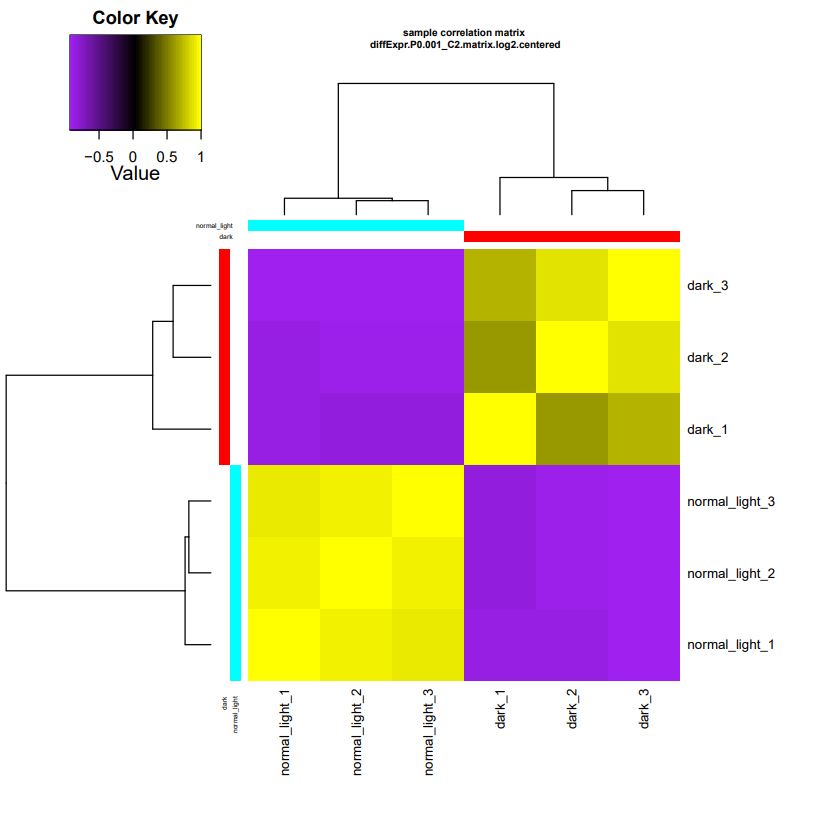
\includegraphics{assets/35_DE_sample_cor.png}

}

\caption{Sample correlation matrix visualized only for differentially
expressed transcripts.}

\end{figure}

\begin{itemize}
\tightlist
\item
  \texttt{diffExpr.P0.001\_C2.matrix.log2.centered.genes\_vs\_samples\_heatmap.pdf}
  is heatmap of differentially expressed transcripts.
\end{itemize}

\begin{figure}

{\centering 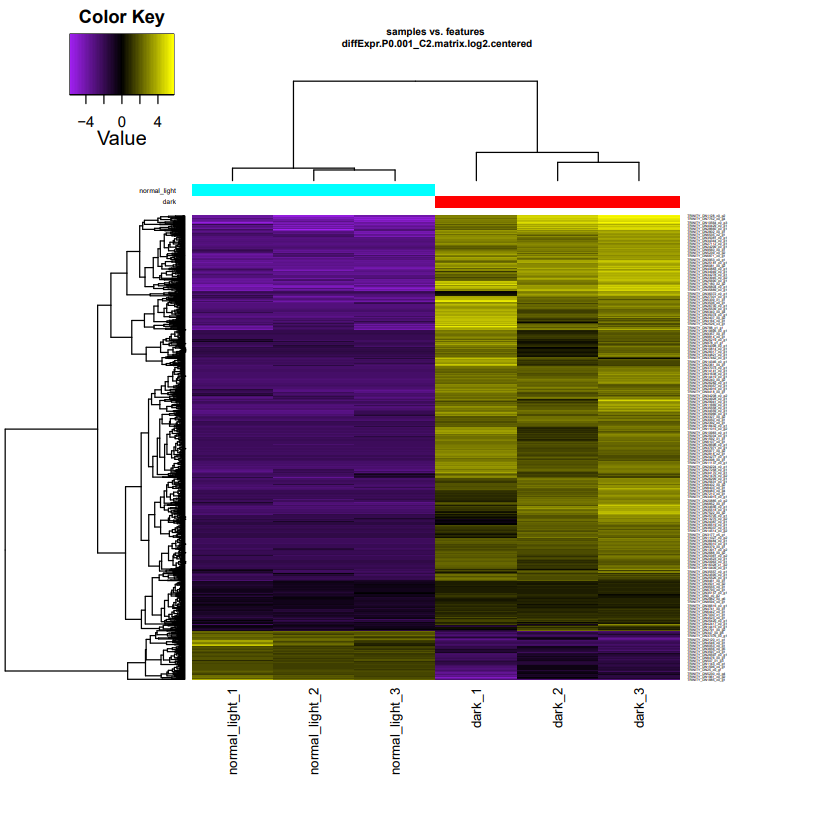
\includegraphics{assets/36_DE_heatmap.png}

}

\caption{Heatmap of differentially expressed transcripts.}

\end{figure}

\hypertarget{de-gene-patterning-and-clustering-analysis}{%
\section{DE gene patterning and clustering
analysis}\label{de-gene-patterning-and-clustering-analysis}}

In the heat map of differentially expressed transcripts, there is a
clear difference between the DE transcripts under dark and normal light
conditions. Therefore, using
\texttt{define\_clusters\_by\_cutting\_tree.pl}, we can divide these
genes into clusters based on the same trend of expression values as
follows.

\begin{tcolorbox}[enhanced jigsaw, breakable, bottomrule=.15mm, left=2mm, coltitle=black, opacityback=0, colframe=quarto-callout-note-color-frame, toprule=.15mm, opacitybacktitle=0.6, colbacktitle=quarto-callout-note-color!10!white, bottomtitle=1mm, colback=white, toptitle=1mm, titlerule=0mm, rightrule=.15mm, arc=.35mm, title=\textcolor{quarto-callout-note-color}{\faInfo}\hspace{0.5em}{Activity}, leftrule=.75mm]

Automatically Partitioning Genes into Expression Clusters

\begin{Shaded}
\begin{Highlighting}[]
\ExtensionTok{define\_clusters\_by\_cutting\_tree.pl} \DataTypeTok{\textbackslash{}}
\NormalTok{{-}R diffExpr.P0.001\_C2.matrix.RData }\DataTypeTok{\textbackslash{}}
\NormalTok{{-}{-}Ptree 60}
\end{Highlighting}
\end{Shaded}

\end{tcolorbox}

There are three different methods for dividing genes into clusters,
K-Means clustering, hierarchical clustering (as used in the heatmap),
and the recommended method of using criteria to truncate tree branch
lengths that fall below the criteria by using `--Ptree'.

The following results will append to the current working directory
\texttt{DESeq2\_result} which are files and
\texttt{diffExpr.P0.001\_C2.matrix.RData.clusters\_fixed\_P\_60/}
directory.

\begin{verbatim}
-rw-rw---- 1 root PSLab    45837 Mar  6 16:51 clusters_fixed_P_60.heatmap.heatmap_gene_order.txt
-rw-rw---- 1 root PSLab    61467 Mar  6 16:51 clusters_fixed_P_60.heatmap.gene_cluster_colors.dat
-rw-rw---- 1 root PSLab   110890 Mar  6 16:51 clusters_fixed_P_60.heatmap.heatmap.pdf
drwxrwx--- 1 root PSLab      400 Mar  6 16:51 diffExpr.P0.001_C2.matrix.RData.clusters_fixed_P_60/
\end{verbatim}

List of files in
\texttt{diffExpr.P0.001\_C2.matrix.RData.clusters\_fixed\_P\_60/}
directory are:

\begin{verbatim}
-rw-rw---- 1 root PSLab  43915 Mar  6 16:51 my_cluster_plots.pdf
-rw-rw---- 1 root PSLab 220780 Mar  6 16:51 subcluster_1_log2_medianCentered_fpkm.matrix
-rw-rw---- 1 root PSLab  26259 Mar  6 16:51 subcluster_2_log2_medianCentered_fpkm.matrix
-rw-rw---- 1 root PSLab    816 Mar  6 16:51 __tmp_plot_clusters.R
\end{verbatim}

The DE transcript partiitoning and clustering is located in
\texttt{my\_cluster\_plots.pdf}

\begin{figure}

{\centering 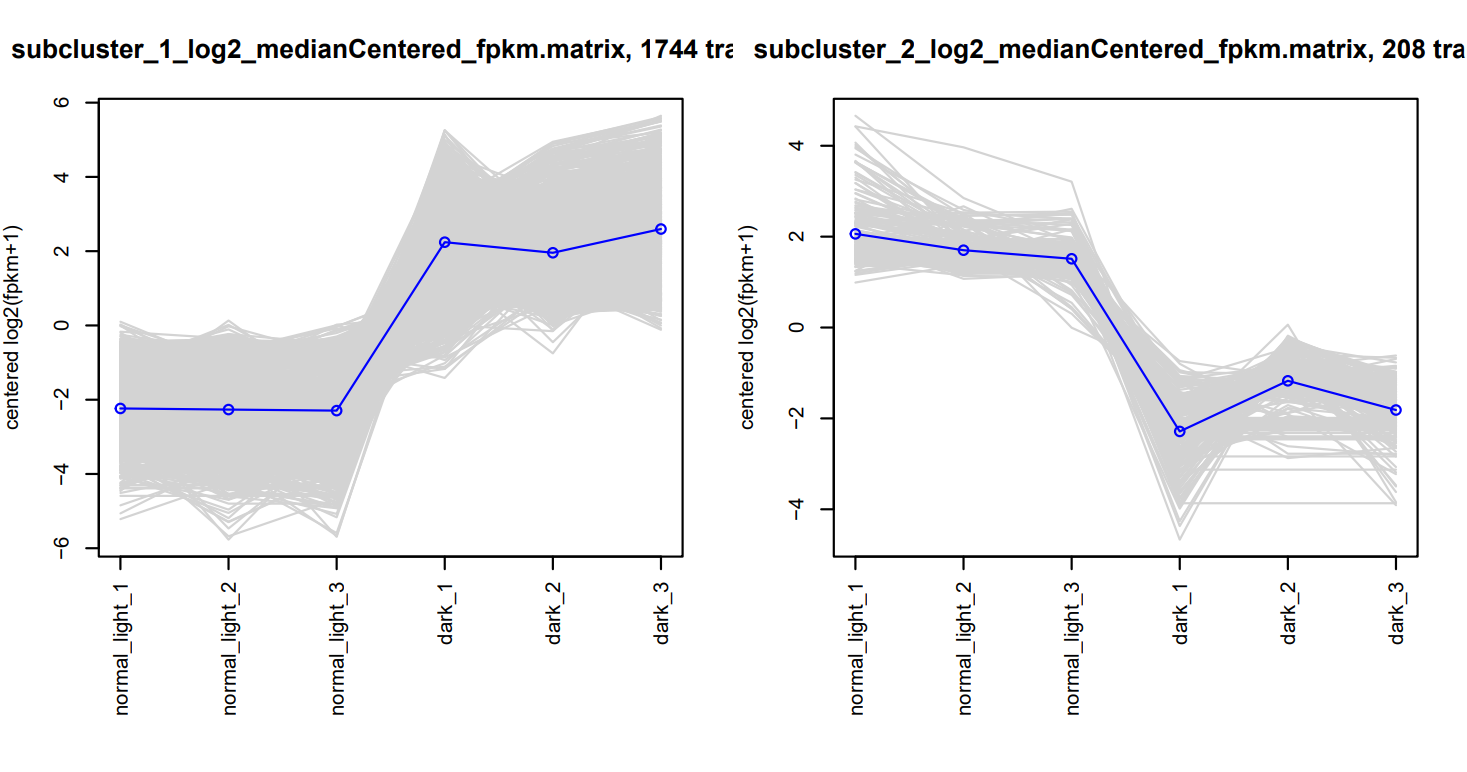
\includegraphics{assets/37_DE_partition.png}

}

\caption{DE transcript partiitoning and clustering analysis}

\end{figure}

\bookmarksetup{startatroot}

\hypertarget{transcriptome-assembly-annotation}{%
\chapter{Transcriptome Assembly
Annotation}\label{transcriptome-assembly-annotation}}

\bookmarksetup{startatroot}

\hypertarget{references}{%
\chapter*{References}\label{references}}
\addcontentsline{toc}{chapter}{References}

\markboth{References}{References}

\hypertarget{refs}{}
\begin{CSLReferences}{1}{0}
\leavevmode\vadjust pre{\hypertarget{ref-grabherr2011}{}}%
Grabherr, Manfred G, Brian J Haas, Moran Yassour, Joshua Z Levin, Dawn A
Thompson, Ido Amit, Xian Adiconis, Lin Fan, Raktima Raychowdhury, and
Qiandong Zeng. 2011. {``Trinity: Reconstructing a Full-Length
Transcriptome Without a Genome from RNA-Seq Data.''} \emph{Nature
Biotechnology} 29 (7): 644.

\leavevmode\vadjust pre{\hypertarget{ref-haas2013}{}}%
Haas, Brian J, Alexie Papanicolaou, Moran Yassour, Manfred Grabherr,
Philip D Blood, Joshua Bowden, Matthew Brian Couger, David Eccles, Bo
Li, and Matthias Lieber. 2013. {``De Novo Transcript Sequence
Reconstruction from RNA-Seq Using the Trinity Platform for Reference
Generation and Analysis.''} \emph{Nature Protocols} 8 (8): 1494--1512.

\leavevmode\vadjust pre{\hypertarget{ref-martin_next-generation_2011}{}}%
Martin, Jeffrey A., and Zhong Wang. 2011. {``Next-Generation
Transcriptome Assembly.''} \emph{Nature Reviews Genetics} 12 (10):
671--82. \url{https://doi.org/10.1038/nrg3068}.

\end{CSLReferences}



\end{document}
